\documentclass[conference]{IEEEtran}
\IEEEoverridecommandlockouts
% The preceding line is only needed to identify funding in the first footnote. If that is unneeded, please comment it out.
\usepackage{cite}
\usepackage{amsmath,amssymb,amsfonts}
\usepackage{algorithmic}
\usepackage{graphicx}
\usepackage{textcomp}
\usepackage{xcolor}
\usepackage{kotex}
\usepackage{float}
\def\BibTeX{{\rm B\kern-.05em{\sc i\kern-.025em b}\kern-.08em
    T\kern-.1667em\lower.7ex\hbox{E}\kern-.125emX}}
\begin{document}

\title{PharmaSEE\\
% {\footnotesize \textsuperscript{*}Note: Sub-titles are not captured in Xplore and
% should not be used}
% \thanks{Identify applicable funding agency here. If none, delete this.}
}

\author{
\IEEEauthorblockN{Dayoung Yun}
\IEEEauthorblockA{\textit{Department of Information Systems}\\
\textit{Hanyang University}\\
Seoul, South  Korea\\
yundayoung1028@gmail.com}
\and
\IEEEauthorblockN{Morgan Jeon}
\IEEEauthorblockA{\textit{Department of Information Systems}\\
\textit{Hanyang University}\\
Seoul, South  Korea\\
momopeach9816@gmail.com}
\and
\IEEEauthorblockN{KyoungWhan Mheen}
\IEEEauthorblockA{\textit{Department of Information Systems}\\
\textit{Hanyang University}\\
Seoul, South  Korea\\
kwmheen@hanyang.ac.kr}
\and
\IEEEauthorblockN{Dohyeong Han}
\IEEEauthorblockA{\textit{Department of Information Systems}\\
\textit{Hanyang University}\\
Seoul, South  Korea\\
dohan2038@gmail.com}
\and
\IEEEauthorblockN{Miju Kang}
\IEEEauthorblockA{\textit{Department of Information Systems}\\
\textit{Hanyang University}\\
Seoul, South  Korea\\
mj0904meeju@gmail.com}
\and
\IEEEauthorblockN{}
}

\maketitle

\begin{abstract}
 PharmaSEE is a service that provides the following two functions. The first is for users to obtain information about the pills through image recognition technology. They can get details about the pills they're taking, and they can even set a dosing time alarm. Also, even if they take several pills at once, you can tell whether the medicines in the picture are the medicines you need to take today or not. The second is that caregivers can check the pill taking records of their parents or patients. The target customers are people who have a hard time knowing exactly which medications to take like elderly people or patients who are physically disabled and their caregivers who feel uncomfortable checking each time that their parent or patient has taken the correct pill. In addition, all these functions can be implemented using artificial intelligence speakers. This makes the application more comfortable for elderly people with relatively poor eyesight. With regards to data resources, we use a pill image dataset provided by the Ministry of Food And Drug Safety of Korea. There may be possible additional features. For instance, it can recommend over-the-counter medicine according to symptoms. Or we can apply this service to nutritional supplements or vitamins.\\
\end{abstract}

\begin{IEEEkeywords}
Image Recognition, Mobile Application, AI Speaker
\\
\\
\\
\\
\\
\\
\\
\\
\\
\\
\\
\\
\\
\\
\\
\\
\\
\\
\\
\\
\\
\\
\\
\\
\\
\\
\\
\\
\\
\\
\\
\\
\\
\\
\\
\\
\\
\\
\\
\\
\\
\\
\\
\\
\\
\\
\\
\\
\\
\\
\\
\\
\\
\\
\\
\\
\\
\\
\\
\\
\\
\\
\\
\\
\\
\end{IEEEkeywords}

\section*{Role Assignment}
\begin{table}[h!]
% \caption{Table Type Styles}
% \begin{center}
\begin{tabular}{|p{0.1\textwidth}|p{0.06\textwidth}|p{0.25\textwidth}|}
\cline{1-3} 
\textbf{Role} & \textbf{\textit{Name}}& \textbf{\textit{Task Description}}\\
\hline
User/Customer&All&The person who plays the role of User/Customer collects information from users necessary for application development through a survey. He determines the main customer of the application. He prepares surveys and interviews. He analyzes the results of surveys and interviews. Based on the analysis of results, the functions and complementary points necessary for application development are shared. \\
\hline
Backend Developer&Dayoung Yun, Dohyeong Han&Backend developers think about backend systems which are needed in developing projects like using databases with SQL queries. We manage the server-side and database related to the process of a website, web application or mobile solution. As a backend developer, as many languages are provided like python, Java, Node.js, JavaScript.\\
\hline
Frontend Developer&Miju Kang,
Morgan Jeon&A frontend developer makes the environments for the users. In this project, the frontend developer also designs the UI/UX for the application. She considers user convenience and implementing design on websites and applications. It is important to hide the bug in the front, so that the user cannot notice the problem. As a frontend developer, the ability to use html, javascript and css is needed.\\
\hline
AI Developer&Kyoung Whan Mheen&The AI developer will make the pipeline that processes images and applies machine learning algorithms to classify the images taken by the user. The AI developer needs to make sure the machine learning model is making plausible predictions and is also responsible for the deployment of the pipeline.\\
\hline
Development Manager&Morgan Jeon&Development manager has to control the whole process of  software development. Therefore, it’s important to communicate with all team members for a development manager. Also,a development manager should read the situation of a market, think up essential services and suggest it to other team members. Finally, the development manager has to listen to and summarize the voice of customers and notify it to developers for service updates.\\
\hline

\end{tabular}
% \label{tab1}
% \end{center}
\end{table}

\begin{figure}[h!]
\caption{Role assignments of team members.}
\label{fig}
\end{figure}

\section{Introduction}

\subsection{Motivation}\label{AA}
\subsubsection{ESG Management}
ESG management refers to the pursuit of management activities that are beneficial to humans and society by solving problems that arise in management activities such as the environment, society, and governance structure, away from growth-oriented corporate activities that emphasized only financial performance in the past.

The concept of ESG management first appeared in 2004 and was declared as the concept of SDGs in 2015. Not only Korea, but the whole world advocates ESG management, and ESG management has become a necessity rather than an option across all industries. Many companies make ESG management-related programs or plan events. In addition, ESG management-related campaigns are launched or ESG management-related products and digital services are introduced to the market.

Consumers say they've seen a rise in liking when they know that a company they've never been interested in before is continuing ESG activities. In addition, some consumers say that they very much prefer companies that practice ESG management in terms of realizing social values and contributing to a just society.

In particular, recently, meaning-out is emerging as a consumption trend. Along with the 'meaning-out' consumption trend that reveals their social values through active consumption behavior, consumers are also interested in realizing ESG values.

In addition, prosumers are emerging in the market recently. A prosumer refers to an independent consumer who goes from passive purchasing to directly participating in the distribution process. As a 'prosumer' who actively consumes, I want to take an independent attitude and take an interest in the distribution process from passive purchasing and participate directly.

Therefore, launching a service that can practice ESG management helps to enhance the image and sales of the company.

Among ESG, we decided to focus on the social sector. Social policies can effectively communicate to consumers. In addition, social values are universal values that all generations can sympathize with. However, in the case of the environment, some people are insensitive to environmental values, and in the case of governance, there are limitations in that it is difficult to deliver values to consumers.

Areas that can be looked at in relation to social issues include support for the underprivileged, medical support, respect for human rights, and improvement of the working environment.Among them, we came to plan a medical support service for the elderly who are underprivileged.\\

\subsubsection{Discomfort when elderly people take pills}
Drugs are essential factors for modern people, from treating diseases to taking vitamins to improve their health. In particular, the elderly often take medicine because of their sick body. In this light, we planned this project to eliminate obstacles that make certain elderly people uncomfortable when taking medicine in their lives.

There are two main cases of taking medicine not periodically. First, it is easy to forget to take them when you have a busy morning or tiring day. Second, the medication interval is also set, but it is easy to take the medication arbitrarily without properly measuring the medication interval. In this situation, we felt that a program was needed to inform elderly people the proper time to take each particular drug.

From a different point of view, the elderly people are a class that feels very uncomfortable taking medicine. They have poor eyesight, so can’t distinguish what drugs they are taking now. Even though there are descriptions of the medicines on the prescription or medicine envelope, because of their poor eyesight, it is not easy to know what kind of medicine they are holding and what kind of efficacy the medicines have. Also, there are many drugs that the elderly take, so it is difficult to distinguish them one by one. Therefore, in order to help them take medicine, we thought that an additional function to recognize the medicine was needed.\\

\subsubsection{Discomfort of children or caregivers checking their parents' medications}
Some elderly people have various physical and mental discomforts. They have poor eyesight or are forgetful. So, they don't remember exactly what medications they take, when they last took them, or how many times they should be taken.

This is a big problem for children who are concerned about their parents' health and caregivers who need to take care of the sick. If the elderly do not take their medications properly, it is difficult to properly manage their body and the disease is difficult to be cured.

Some people check to see if they have taken the medicine through phone calls or messages, but it is difficult to check frequently due to the nature of the medicine that needs to be taken three times a day, and it is impossible to know for sure whether the correct medicine was actually taken on time. We devised a function that can solve this inconvenience.\\

\subsection{Problem statement(user's needs)}
- Users often tend to forget the medicine they need to take.\\

- Users can check drug information through the app when the name of the drug is difficult or the manual is lost or hard to read. Drug information includes the name, intake method, expiration date, and side effects of the drug.\\

- Users can check the interaction between taking drugs to prevent the risk of wrong intake.\\

- Users can prevent duplicate intake by leaving records of taking drugs.\\

- Users can distinguish which medications to take at a given time from among the various medications they need to take. \\

- Users can check and manage if their parents or patients are taking their medications properly.\\

\subsection{Research on related  software}
\subsubsection{Korea Pharmaceutical Information Center}
The Korean Pharmaceutical Information Center provides pill searching services on their websites. People can search the pill by its shape, color, and formulation. After selecting the shape and color, the website shows the pills that meet the conditions. The name, company and ingredient of the pill is provided in the website, but the effect of the pill is not included. Also, it does not provide a system for the people who are visually impaired.\\

\subsubsection{HealthMore}
HealthMore is an application for people who are visually impaired. It is provided in the  iPhone Appstore and Google Playstore. In the application, people can take the photo of the barcode of drugs and get the information. Also, the information of pills in a prescription can be informed if the prescription includes a QR code. When people take the photo of the QR code in the prescription, the list of the pills, name of the hospital and doctor, and the date medicines prescribed  can be known. The application also provides searching functions in voice or text. If a user presents his personal health information, the caution for some drugs that are not good for him is also provided.\\

\subsubsection{Pill Reminder Drug Alert}
Pill Reminder Drug Alert is an application that helps user eat his or her medications on time. Enter the name of the drug, the dosage, the first dose, and the time interval. User can also customize his or her medications by color or sound. It is convenient to use if users have problems taking or overdosing on medications. Allows users to take their medications at the right time. Users may be notified of the next dose time. However, this application does not have a photo recognition and search function, and only sends a notification after the user registers directly. It doesn't give users any information about the drug. Communication between different users is also impossible.\\

\subsubsection{Pill Reminder}
In Pill Reminder, users can reserve all their medicines in one app. It is possible to designate the pill with a picture and name. Users can check the next dose and receive a notification. The users can also take notes on medications, write dosages, and even have personalized reminders. However, there is no search function for pills, and notifications are sent only to the user, not the child or caregiver.\\

\subsubsection{Parental Love Hyodol}
Parental Love Hyodol is an application that allows you to manage your parents' situation. Users can check the activity of their parents in real time. In addition, users can turn on notifications to quickly respond to emergency situations. Families can receive emergency alerts when parental movements are not detected for more than the time set in the app, so they can respond quickly to emergencies. Users can also record voice messages directly from the app and send them through the app. The whole family can connect with their parents together, so the whole family can check the status of their parents and convey their feelings. In the schedule management function, the parent's medical visit schedule, such as a hospital, dentistry, oriental clinic, may be registered as a reminder.However, in this application, users cannot manage their parents' medication.\\

\subsubsection{Age of Parents}
Age of Parents provides patient caregivers who want hospitalized families to recuperate in a healthy and comfortable environment in a comfortable environment, providing a service that allows them to check the patient's treatment, various activity programs, and activity photos. You can see who is connected to the hospitalized family or parents' health information. You can also see photos of their daily life. You can also find out what treatment your hospitalized family members are getting and what kind of diet they are eating. In addition, you can check the schedule of various activities and events of the hospital or nursing facility, and you can check the composition of patients in the ward and the status of the facility. However, in this app, it is also not possible to know what medications the parents are taking or whether they have taken good care of them.\\

\section{Requirement Analysis}
\subsection{Mobile Application}\label{AA}
Users can access the main services provided by PharmaSEE through a mobile application. Native applications for Android and iOS will be provided. The user can access services such as pill image recognition, personal medication list, medication intake calendar and personalized notifications. The mobile app will be connected to a cross-platform backend server that will also communicate with the NUGU device in order to provide voice assistance for users that are not used to the mobile interface. The main functions of the mobile application are as follows.\\
\paragraph{Loading UI}The users will see a loading UI while waiting for the mobile app to boot. The PharmaSEE logo and a simple animation will indicate the user to wait for the loading process to complete.\\

\paragraph{Navigation Tab}There are several menus the user has to navigate through while using the mobile application. A navigation tab will allow the user to shift between different menus. \\

\paragraph{Main Page}The main page will display the menu icons to navigate to ‘Pill Search’, ‘Pill Box’, etc. This will be the first page users will see upon entering the mobile application.\\

\paragraph{Search Pill}Users can navigate to the pill search menu in order to identify an unknown medicine and acquire information about it. The mobile application will open the smartphone’s built-in camera and wait for the user to take an image of the pill.\\

\paragraph{Pill Information Display}After the pill has been recognized and analyzed through the image recognition model, information about the pill will be queried from the database through the backend server. The queried information contains data such as the name and effects. The information will be displayed in text. Also, users will be able to add the identified pill to their own pill box.\\

\paragraph{Pill Box}Another important feature of PharmaSEE is the ‘Pill Box’ section. The users can register to a list the pills they need to take daily. They can check detailed informations about the pills. Also, they can set a notification alarm to remind them to take the pill.\\

\begin{itemize}

\item List: The user can check a list of pills that they are taking now. The pills registered by users are automatically added to the list. In addition, at the end of the period of taking a pill, it may automatically disappear from the list.\\ 

\item Information : The users can see more details about the pills they are taking such as name, manufacturer(a medicine company that made the pill), proper usage and dose, effects,possible side effects, etc.\\

\item Alarm Setting: Users can set frequency of their notifications which alert the time to take medicines.\\
\end{itemize}

\paragraph{Today's Pill}
When users take a picture of the pill they're trying to take and post it, they'll get a notification and a picture back telling them whether the drug is the drug they need to take now or not.\\

\paragraph{Link Caregivers}
Users can find and follow their caregivers. Followed caregivers can check the pill administration information of their wards.\\

\subsection{Nugu Interface}
The PharmaSEE mobile application requires a voice interface for the user. This voice interface will allow users to query their intake information. Caretakers will also be able to query information about their ward's medication intake. This allows the users to view intake information through various mediums, making the medical care service experience much more convenient. \\ \\
The Nugu interface will be built using the Nugu play builder platform. Through the nugu builder platform, custom intents and actions specific to our target customers will be created and a backend proxy server containing user data will be developed and deployed. The main utilities provided through the Nugu interface will be to ask about the pills that the users had took today, and to ask about pills that has been forgotten or has to be taken in the future. \\

\paragraph{Ask Taken Pills}
The users may forget exactly what pills they have taken before. In this case they can open the PharmaSEE mobile application to check, but it would be more convenient for them to just ask through voice. In order to serve this need, the Nugu interface will interpret user utterances such as 'PharmaSEE, what pills did I take today?' and respond accordingly. The Nugu device will send a request to the backend server for an answer on the qeustion. A response similar to this will be sent from the backend server and played to the user through Nugu. \\ \\
'You (He/She if the user is the caretaker) took 1 dose of pillA at 11am today. This is 2 hours later than the scheduled time so please take caution.'. \\

\paragraph{Ask Not Taken Pills}
More important than to remeber what pills were taken on that day is to be reminded if there are any pills that the user forgot to intake. Also the user should be informed that there are pills scheduled to be taken in the future. To serve this need, the Nugu interface will interpret user utterances such as 'PharmaSEE, are they any pills I forgot to take today?' and respond accordingly. The Nugu device will reqeust the backend server for information on the pills the user has not taken. A response similar to this will be sent from the backend server and played to the user through Nugu. \\ \\
'You (He/She if the user is the caretaker) forgot to take 1 dose of pillA iat 11am today. Also, you are scheduled to take 2 doses pillB later at 9pm today, so please do not forget.'.\\
\\
\\
\\
\\
\\
\\
\\
\\
\\
\\
\\
\\
\\
\\
\\
\\
\\
\\
\\
\\
\\
\\
\\
\\
\\
\\
\section{Development Environment}
\subsection{Choice of software development platform}\label{AA}
\subsubsection{Which platform and why?}
We will develop a mobile application on Windows. Our service is a kind of healthcare application, so it should be ready at hand. So our service provides a mobile application for users. We will develop both iOS and Android, so we should choose a cross-platform available technology stack. React Native will be used to develop the application. By using React Native, both Android and iOS will be supported in the same codebase. It means that we can support 99.65\% of people in Korea. \\
We will use linux based ubuntu of AWS's EC2 service as server computer. Nginx will be used as a web server. As Django cannot directly communicate with web server, we will use uWSGI python package to connect Django and web server. 


\begin{figure}[h!]
\centering
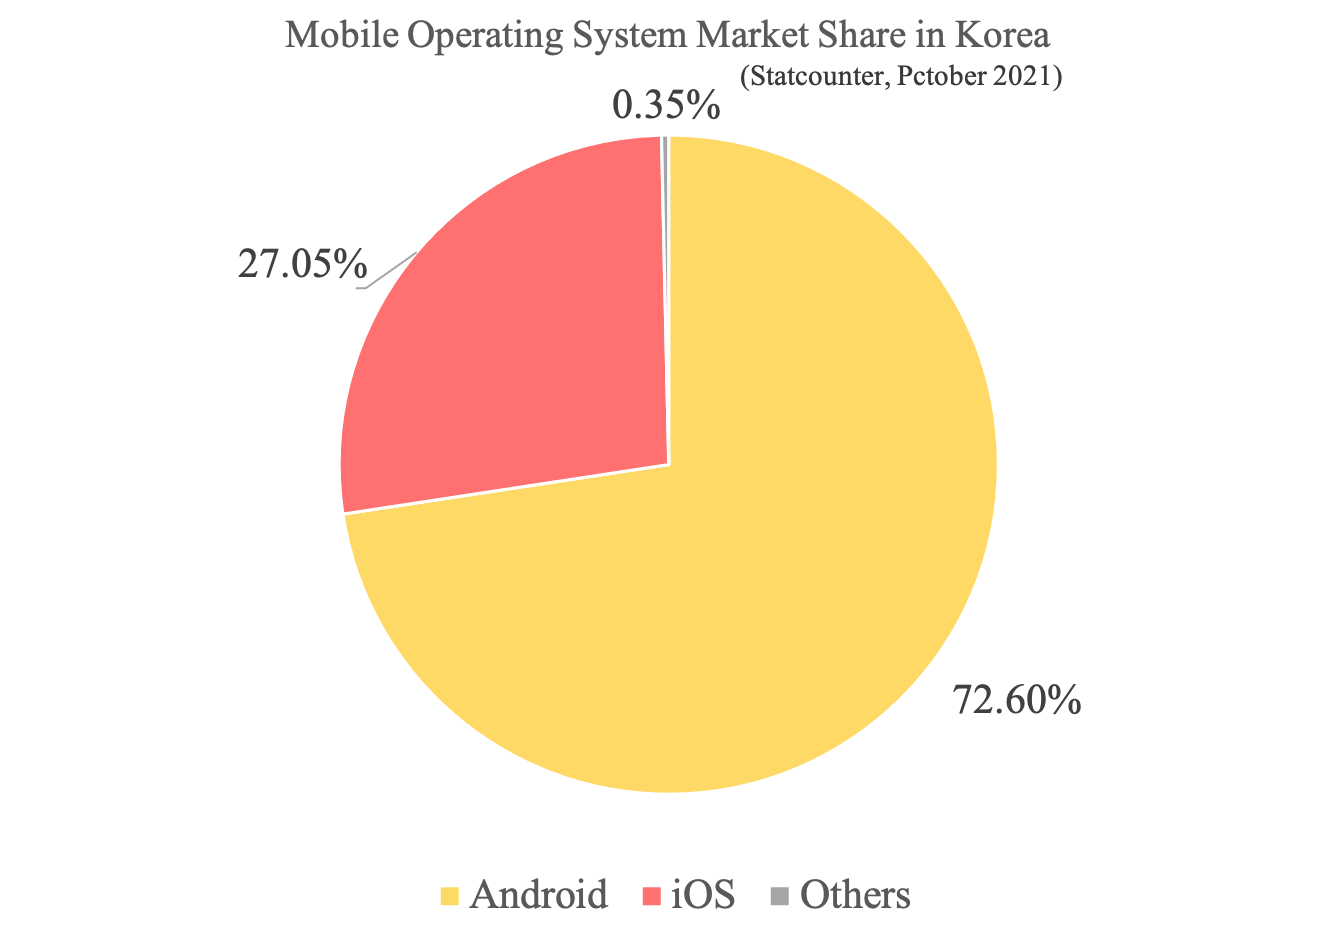
\includegraphics[width=7cm]{imagefolder/1.png}
\caption{}
\label{fig:map}
\end{figure}


\subsubsection{Which programming language and why?}
\begin{table}[b!]
% \caption{Table Type Styles}
\begin{center}
\begin{tabular}{|p{0.1\textwidth}|p{0.25\textwidth}|}
\cline{1-2}
\textbf{Language} & \textbf{\textit{Description}} \\
\hline
Python&Python is script, dynamic type, platform independent language. 
We can check, modify, and write code immediately by the interpreter without the compilation process.
We can develop in any environment such as Windows, Linux, Mac os. 
Python has a low running curve and high scalability and portability. 
Because data learning algorithms will be implemented in a python environment, python has the advantage that it has an extensive set of libraries for artificial intelligence and machine learning. For example, Pandas library for general-purpose data analysis, Seaborn  for data visualization, and Keras, TensorFlow, Pytorch for machine learning. In addition, it is considered advantageous in that a community for problem solving is well established.\\
\hline
JSX&JSX is a JavaScript Extension Syntax used in React to easily write HTML and JavaScript together. It is usually used in React Native and also ReactJS. It is faster than normal JavaScript because it optimizes the codes while translating it to JavaScript. JSX is easy to read because it is similar to html. It is also comfortable for people who have experience in xml or JavaScript. Developers can configure the screen by components, and it increases productivity. In JSX, JavaScript expressions can be also used. \\
\hline
\end{tabular}
\label{tab1}
\end{center}
\end{table}


\subsubsection{Provide a cost estimation for your built}\;

\begin{table}[h!]
% \caption{Table Type Styles}
\begin{center}
\begin{tabular}{|c|c|}
\cline{1-2}
\textbf{Device} & \textbf{\textit{Price(won)}} \\
\hline
Server(AWS lightsail)& Not estimated yet\\ 
\hline
\end{tabular}
\label{tab1}
\end{center}
\end{table}


\subsubsection{Provide clear information about your development environment}
\begin{itemize}
  \item Pill Data Learning Model \\
It will be implemented in macOS 11.6.1 environment (Big Sur). The development will proceed in a Python virtual environment. To create a data learning model, the Python version will be downgraded to 3.7.11 for Tensorflow operation. 
  \item React Native 0.66.3
  \item Node.js 16.13.0
  \item npm 8.1.0
  \item Windows 10
  \begin{itemize}
         \item 1.80 GHz Intel i7
         \item 8GB Memory
       \end{itemize}
  \item MacOS 11.6.1(Big Sur)
  \item Visual Studio Code 1.62.1
  \item Django 3.2.9
  \item AWS EC2 instance
  \item Nginx 1.21.4
  \item Git 2.33.1
\end{itemize}

\subsection{Software in use}\label{AA}
\subsubsection{React Native}
React Native is an open source mobile application framework released by Facebook. It uses ReactJS libraries and JSX. Developers can make an application that is available for both  iOS and Android by using React Native. React Native applications can be used for both platforms simultaneously while using a single codebase. It increases productivity and makes development efficient. React Native optimizes performance by communicating with native thread through the native bridge. \\

\begin{figure}[h!]
\centering

\includegraphics[width=5cm]{imagefolder/react_native.png}
\caption{}
\label{fig:map}
\end{figure}

\subsubsection{Expo}
Expo is a build tool for developing React Native cross-platform. The biggest advantage of Expo is that it can be developed while testing the app under development on a mobile screen. In addition, if you use Expo, you can develop apps without installing Android Studio or iOS development programs yourself. Expo makes it easier and more convenient to use native modules.

\begin{figure}[h!]
\centering
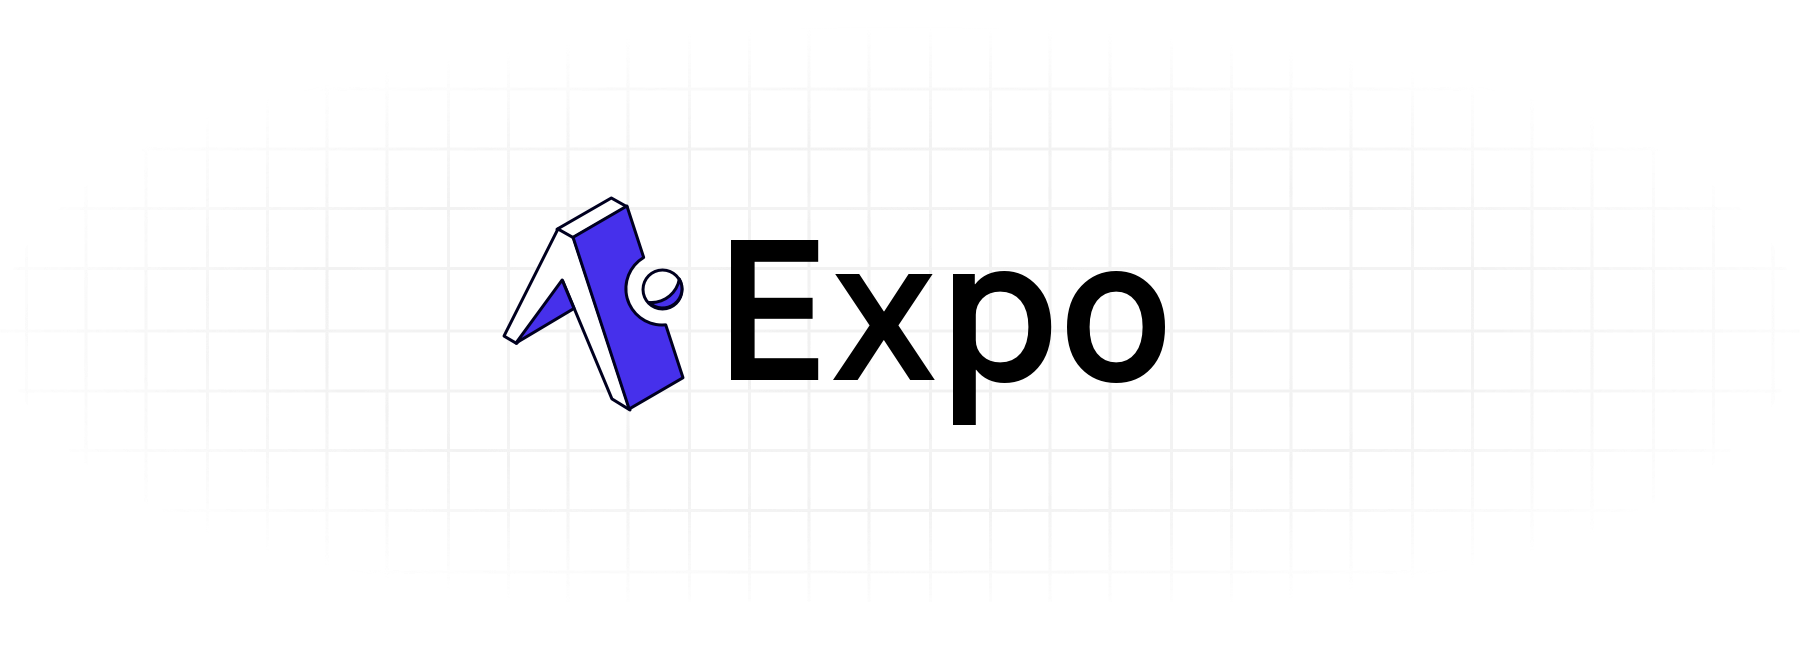
\includegraphics[width=5cm]{imagefolder/expo.png}
\caption{}
\label{fig:map}
\end{figure}

\subsubsection{Django}
Django is a full-stack open-source framework that can be developed both in the front-end and the back-end. Django provides ORMs that connect RDBs(relational databases) such as SQLite, PostgreSQL, MySQL, and Oracle with objects without using SQL queries.  Django has an active community where we can obtain information when a problem occurs. Django provides an administrator page to easily generate and change data. Django also takes care of user authentication, content administration, site maps and many more tasks out of the box. \\

\begin{figure}[h!]
\centering

\includegraphics[width=5cm]{imagefolder/django.png}
\caption{}
\label{fig:map}
\end{figure}

\subsubsection{TensorFlow}
TensorFlow, created in 2015 by Google Brain Team, is an open source software library for data flow programming for various tasks. It is a symbolic math library and is also used in machine learning applications such as artificial neural networks and deep learning. \\
Also It has compatibility with Keras, which is an open source neural network library. Keras provides pipelining, estimators, and eager execution which are system-specific functionality to TenseFlow. Keras functional API supports a variety of topologies with different combinations of I/O, and layers. \\
\begin{figure}[h!]
\centering

\includegraphics[width=5cm]{imagefolder/tensor.png}
\caption{}
\label{fig:map}
\end{figure}

\subsubsection{OpenCV}
OpenCV is a open source library of programming functions mainly aimed at computer vision and machine learning. The library has more than 2500 optimized algorithms, which includes a comprehensive set of both classic and state-of-the-art computer vision and machine learning algorithms. These algorithms can be used to detect and recognize faces, identify objects, classify human actions in videos, track camera movements, track moving objects, etc.\\ 
OpenCV is written in C++ and it has bindings for Python, Java and MATLAB. Also, it works on various interfaces such as Windows, Linux, MacOS and Android. The OpenCV Python API is a wrapper around C++ code and uses NumPy operations internally, allowing users to run python computer vision code without performance issues. \\


\begin{figure}[hbt!]

\includegraphics[width=5cm]{imagefolder/opencv.png}
\caption{}
\label{fig:map}
\end{figure}

\subsubsection{Git, Github}
Git is a tool that can manage project versions. We can copy the project to our local environment and merge it again after working. Git provides an environment where multiple people can work as a single project. Providing such an environment can speed up development and manage work details in parallel. And it can increase the stability of the project. Remote storage is required to push files committed with Git. At this time, Github is used as a remote storage. And we can also use Github as a private repository.\\
\begin{figure}[h!]
\centering

\includegraphics[width=5cm]{imagefolder/github.jpg}
\caption{}
\label{fig:map}
\end{figure}

\subsubsection{PostgreSQL}
PostgreSQL is an open source ORDBMS developed by The PostgreSQL Global Development Group. It was first released in 1996. The global usage rate is 4th after the top 3 DBs (Oracle DB, MySQL, Microsoft SQL), and it is characterized by a steady rise.
Compared to MySQL, it supports the SQL standard better, has more powerful features, and performs better as the query becomes more complex. In particular, geospatial query through PostGIS is more powerful than Oracle, and by using Citus extension, parallel indexing, which has been pointed out as a weakness, can be easily processed.\\
\\
\\
\\
\\
\\
\begin{figure}[h!]
\centering
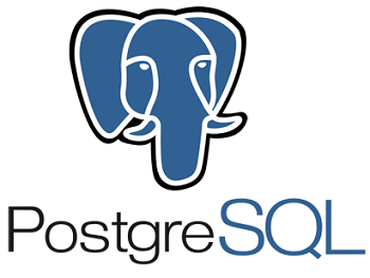
\includegraphics[width=5cm]{imagefolder/postgresql.png}
\caption{}
\label{fig:map}
\end{figure}

\subsubsection{Amazon Lightsail}
Lightsail is the easiest way to start AWS, offering virtual servers, storage, databases and networking as well as a cost-effective monthly plan. It is designed to start small at first and then expand as the business grows.
After creating and running an instance, we can use a browser-based SSH terminal to connect to it via SSH in the Lightsail console.\\
\begin{figure}[h!]
\centering

\includegraphics[width=5cm]{imagefolder/amazon.png}
\caption{}
\label{fig:map}
\end{figure}

\subsubsection{Docker}
Docker is one of the container technologies created using the kernel container technology called LXC. It is becoming the de facto industry standard for Linux container technology.\\
As it is a container technology that does not virtualize the operating system, it is lighter than a virtual machine, and it is good to run multiple services on one server including VMs. Also, since it is an isolated structure that does not easily affect the original server even if the service is hacked for security reasons, the advantages of virtualization can be utilized to a large extent. Unlike virtual machines (VMs), existing Linux resources (disk, network, etc.) can be used as it is, so it is good to drive several services into one server and run them.
\begin{figure}[h!]
\centering

\includegraphics[width=5cm]{imagefolder/docker.png}
\caption{}
\label{fig:map}
\end{figure}

\subsubsection{Postman}
Postman is an API platform for building and testing web APIs during development. Postman is an HTTP client that can send various REST API requests in the form of GET, POST, PUT, DELETE, and PATCH. Developers can save time testing their API servers through the command line and use the graphical user interface provided by Postman. Different types of responses will be displayed through Postman and subsequently validated. Postman also has a feature called 'collections' which allows a team to group requests and organize testing. These collections are folders where requests can be stored and can be structures in whatever way a team prefers. 

\begin{figure}[hbt!]

\includegraphics[width=5cm]{imagefolder/postman.png}
\caption{}
\label{fig:map}
\end{figure}

\subsubsection{Ngrok}
The class-platform application Ngrok allows web developers to expose their local development server to be accessed by external networks with minimal effort. With Ngrok, a locally-hosted web server can appear to be hosted at a subdomain of ngrok.com. This means that no public IP or domain name on the local machine is required. This takes away the troubles of having to do Reverse SSH tunneling as the developers don't need to care about the complicated settings and hosting of a remote server. Ngrok is able to bypass NAT Mapping and firewall restrictions by creating a long-lived TCP tunnel from a randomly generated subdomain on ngrok.com to the local machine. After specifying the port that your web server listens on, the ngrok client program initiates a secure connection to the ngrok server and then anyone can make requests to your local server with the unique ngrok tunnel address. One praised feature of ngrok is the ability to track and replay HTTP requests via ngrok's web console . The replay functionality is highly useful when testing API calls or webhooks as one can easily inspect all header content and request/response data in one place via the console UI.\\
\\
\\

\begin{figure}[h!]

\includegraphics[width=5cm]{imagefolder/ngrok.png}
\caption{}
\label{fig:map}
\end{figure}

\subsubsection{Overleaf}
Through Overleaf that a collaborative cloud-based LaTeX editor users can write, edit and publish scientific documents. As a type of document creation tool, LaTeX is a system used to create special format documents such as thesis or publication. It is a useful document authoring tool for scholars who draw a lot of formulas, graphs, and diagrams in the natural sciences or humanities. LaTeX proceeds with the concept of deriving a result when the entire text structure is put together in a text document written according to specific standards, the content of the text and the symbols indicating the corresponding format, and submitted to the program. Just like creating an executable file by running the compiler after writing the source, you can think of it as creating a document source and running the compiler to create a document or PDF. In addition to page numbers, users can easily implement essential elements necessary for publication grade, such as footnotes, endnotes, table of contents, references, page layouts, tables, and inserting figures. Especially, since documents are written in text files rather than binary, there is an advantage in configuration management with a version control system such as Git.\\
\begin{figure}[h!]
\centering

\includegraphics[width=5cm]{imagefolder/overleaf.png}
\caption{}
\label{fig:map}
\end{figure}

\subsubsection{Slack}
Slack is a cloud-based collaboration tool developed by Stuart Butterfield. The interface for chat, channels, and workplaces is similar to that of Discord, an instant messenger. However, unlike Discord, which focuses on real-time communication for gamers, Slack is more of a work tool for developers and office workers. In fact, various plug-ins are supported so that functions necessary for work can be linked and used. There are functions such as notifying you when there is a push in the GitHub repository, or notifying you in real time by linking a project management tool such as Redmine. Compared to Discord, Markdown is well supported, so Slack is convenient for developers. Slack was used for collaborative communication between team members, and a team project was carried out by creating channels and scrum channels for each area of front-end, back-end, and artificial intelligence. All team members can enter each channel and check the progress of software development.\\

\begin{figure}[h!]
\centering

\includegraphics[width=5cm]{imagefolder/slack.png}
\caption{}
\label{fig:map}
\end{figure}

\subsubsection{Discord}
Discord is an instant messenger that supports voice, chat, and video calls. We used Discord for team voice meetings. Discord provides simple and fast voice chat for general users, and intuitive functions such as overlays, compared to Slack, which is for business.\\
\\
\\
\\
\\
\\
\\
\\
\\
\\
\\

\begin{figure}[t!]
\centering

\includegraphics[width=5cm]{imagefolder/discord.png}
\caption{}
\label{fig:map}
\end{figure}

\subsubsection{Notion}
Notion is a comprehensive memo service that integrates notes, documents, knowledge organization, tasks, projects, and databases into one service. The moment text is edited, it is synchronized on other devices in real time, which is advantageous for collaboration. Pages can be created as sub-items with little or no limitation. It is the same concept as folders can be placed inside folders when organizing files. Because it adopts a familiar method, it is easy to organize the contents by subject. The moving operation can be handled by dragging as in the drag-and-drop method..\\
\\
\\

\begin{figure}[h!]
\centering

\includegraphics[width=5cm]{imagefolder/notion.png}
\caption{}
\label{fig:map}
\end{figure}


\subsection{Task Distribution}\;


\begin{table}[t!]
\begin{center}
\begin{tabular}{|p{0.1\textwidth}|p{0.25\textwidth}|}
\cline{1-2} 
\textbf{Name} & \textbf{\textit{Task Distribution}} \\
\hline
Dayoung Yun&Build the server - Mainly focus on building a pipeline for the pill image recognition service and nugu backens proxy.\\
\hline
Dohyeong Han&Build the server, design API, manage DB. Manage the whole backend part.\\
\hline
Miju Kang&Connect the server and the mobile application. Configure the operation of the mobile application with the data received from the server.\\
\hline
Morgan Jeon&Let the received data be adjusted, construct the User Interface and design it by using CSS.\\
\hline
KyoungWhan Mheen&Based on the collected pill data, a code is created to analyze what the pill is taken in the picture, and send the result value to the server.\\
\hline
\end{tabular}
\label{tab1}
\end{center}
\end{table}


\section{SPECIFICATIONS}\\

\subsection{LOADING UI}\;
Loading UI contains our application’s logo and a background image that can give stability and intimacy to our users. \\

\begin{figure}[h!]
\centering
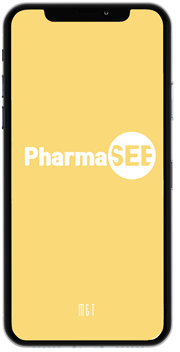
\includegraphics[width=5cm]{imagefolder/loadingui.png}
\caption{}
\label{fig:map}
\end{figure}
.\\
\\
\\
\\
\\

\subsection{MAIN PAGE}
Main Page greets the user. It shows the user's name and profile picture. It also lists up the medications to be taken today. The name of the drug and a green check mark that notice whether the drug was taken are included in the list. Also, main page include a button to update information. \\

\begin{figure}[h!]
\centering
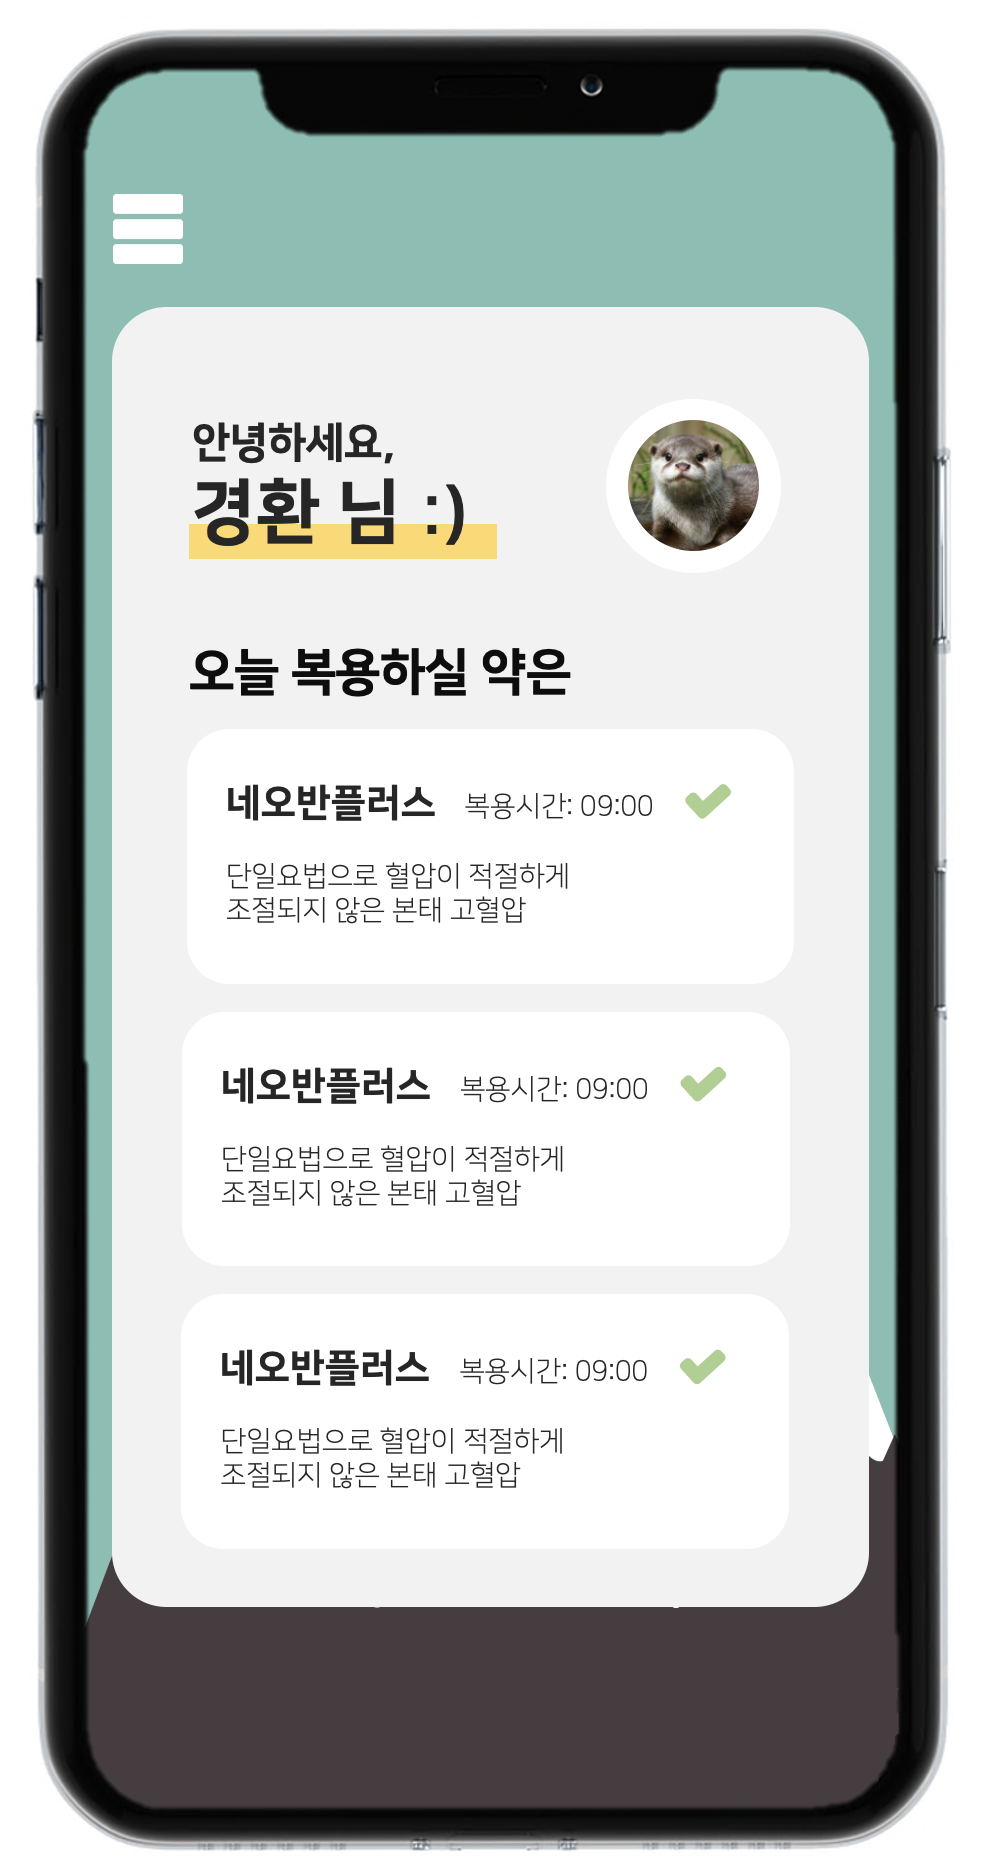
\includegraphics[width=5cm]{final_image_folder/mypage.png}
\caption{}
\label{fig:map}
\end{figure}

.\\
\\
\\
\\
\\
\\
\\
\\
\\
\\
\\
\\
\\
\\
\\
\\
\\
\\
\\

\subsection{Navigation Bar}
Navigation Bar contains the menus in our application. It includes five things below.\\
\begin{itemize}
  \item Main Page
  \item Search/Register Pills
  \item Pill Box
  \item Today's Pills
  \item Caregiver Links
\end{itemize}

When a user clicks a desired function on the navigation bar, it moves to the corresponding page.\\

\begin{figure}[h!]
\centering
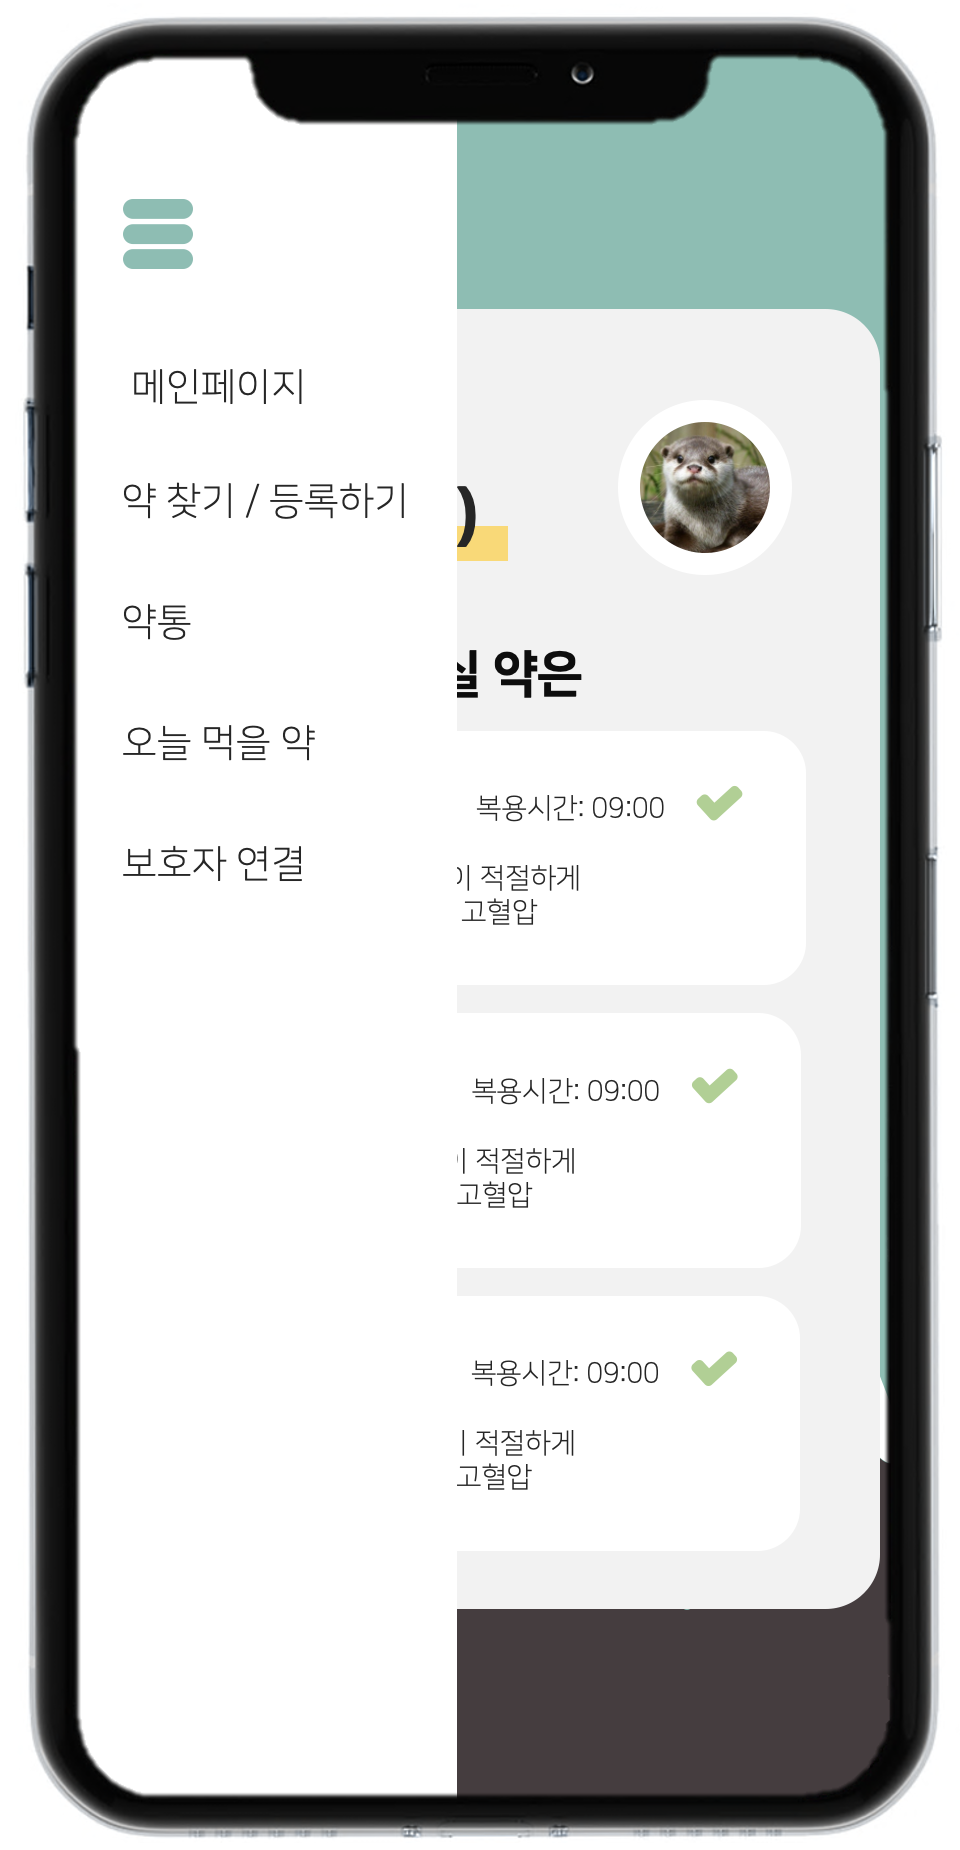
\includegraphics[width=5cm]{final_image_folder/navibar.png}
\caption{}
\label{fig:map}
\end{figure} 

.\\
\\
\\
\\
\\
\\
\\
\\
\\
\\
\\
\\
\\
\\


\subsection{Search/Register Pills}\\

\subsubsection{Before Searching}
There are three ways to search for pills. The first is to search for symptoms. If you search for a symptom, it will show you the pills associated with it. The second is to search by name. Users can search for a drug by entering the name of the drug. The third is to search by photo. User can take a photo, send it to PharmaSEE's server and get information of pills recognized to be the same as the pills in the photo.\\

\begin{figure}[h!]
\centering
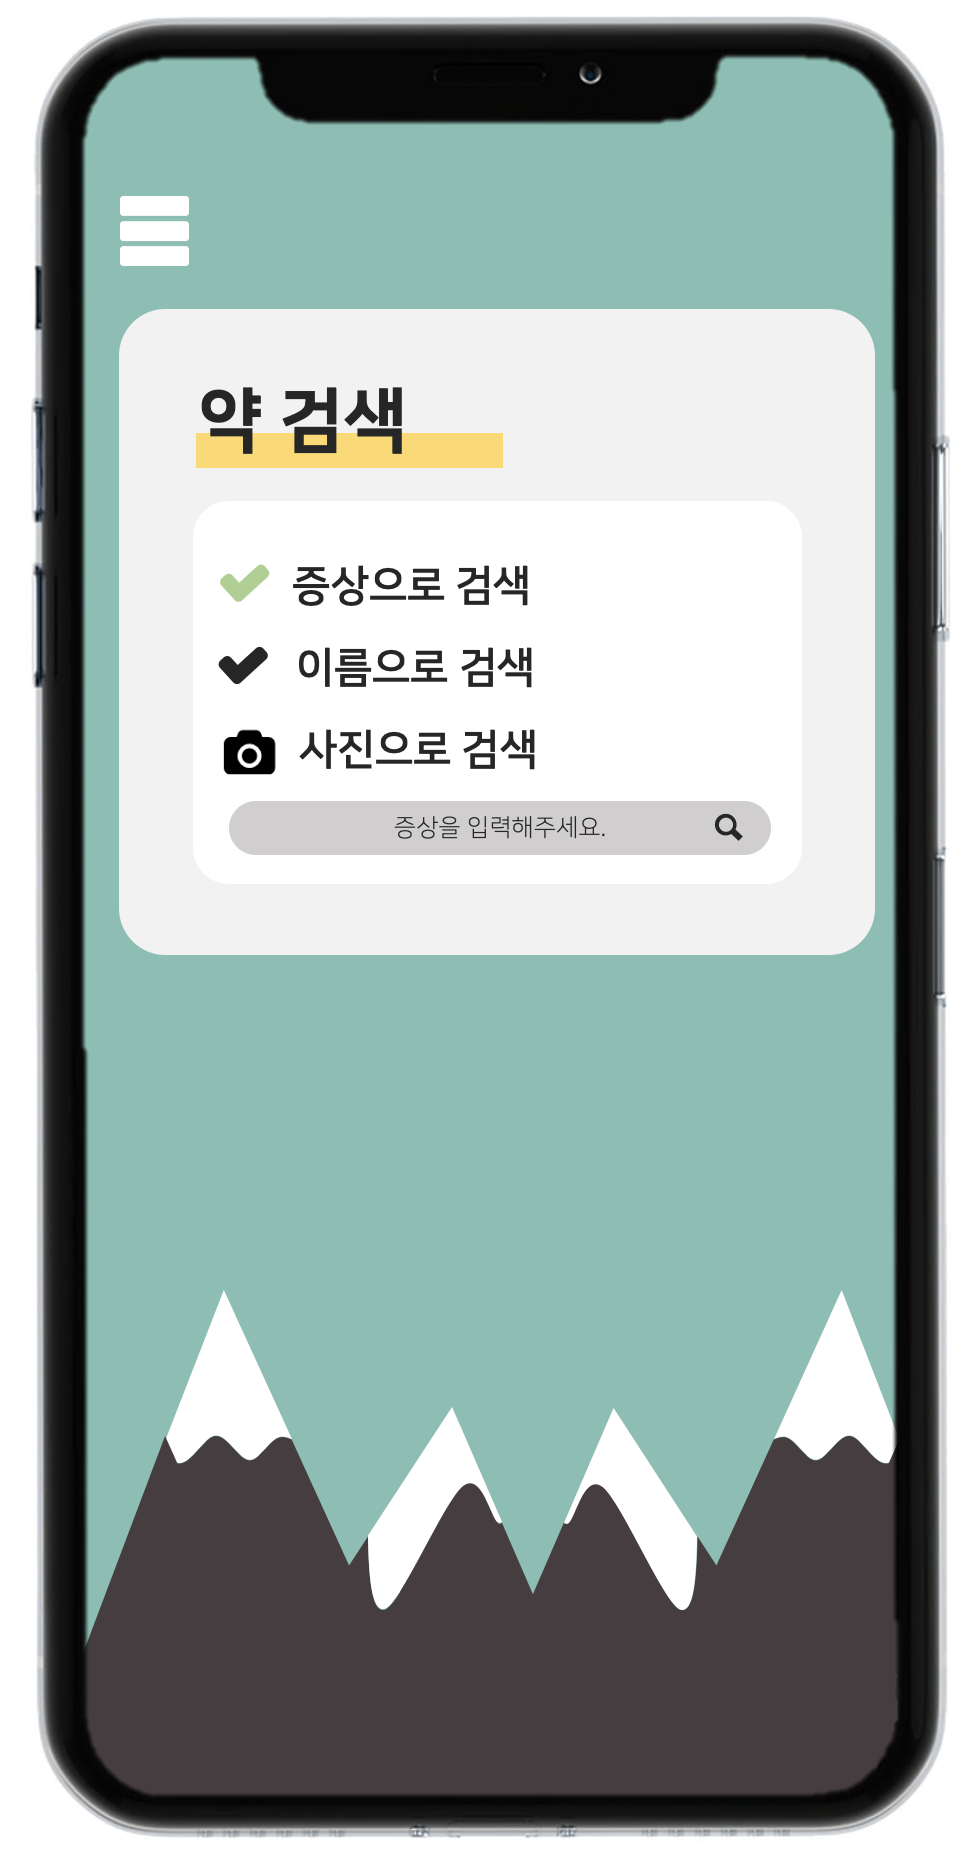
\includegraphics[width=5cm]{final_image_folder/search.png}
\caption{}
\label{fig:map}
\end{figure}

\subsubsection{After Searching - By Symptom or Name}
When a user searches for pills by symptom or name, search word goes to the server. When it's replied by server, the related pills are displayed in the most relevant order. Users can scroll down to see the pill they are looking for. Users can just search other pills by clicking the search bar again.\\ 

\subsubsection{After Searching - By Photo}
After taking the photo of the pill, the image goes to the server and the server recognizes the pill. Recognition of pills in photos is carried out by a program using AI.\\

\subsubsection{Information}
Users can see the name, company, effects, side effects and dosage of the pill in text. When the user presses the 'Add to pill box' button at the bottom of the pill information, the corresponding pill is added to their own pill box.\\ 

\begin{figure}[h!]
\centering
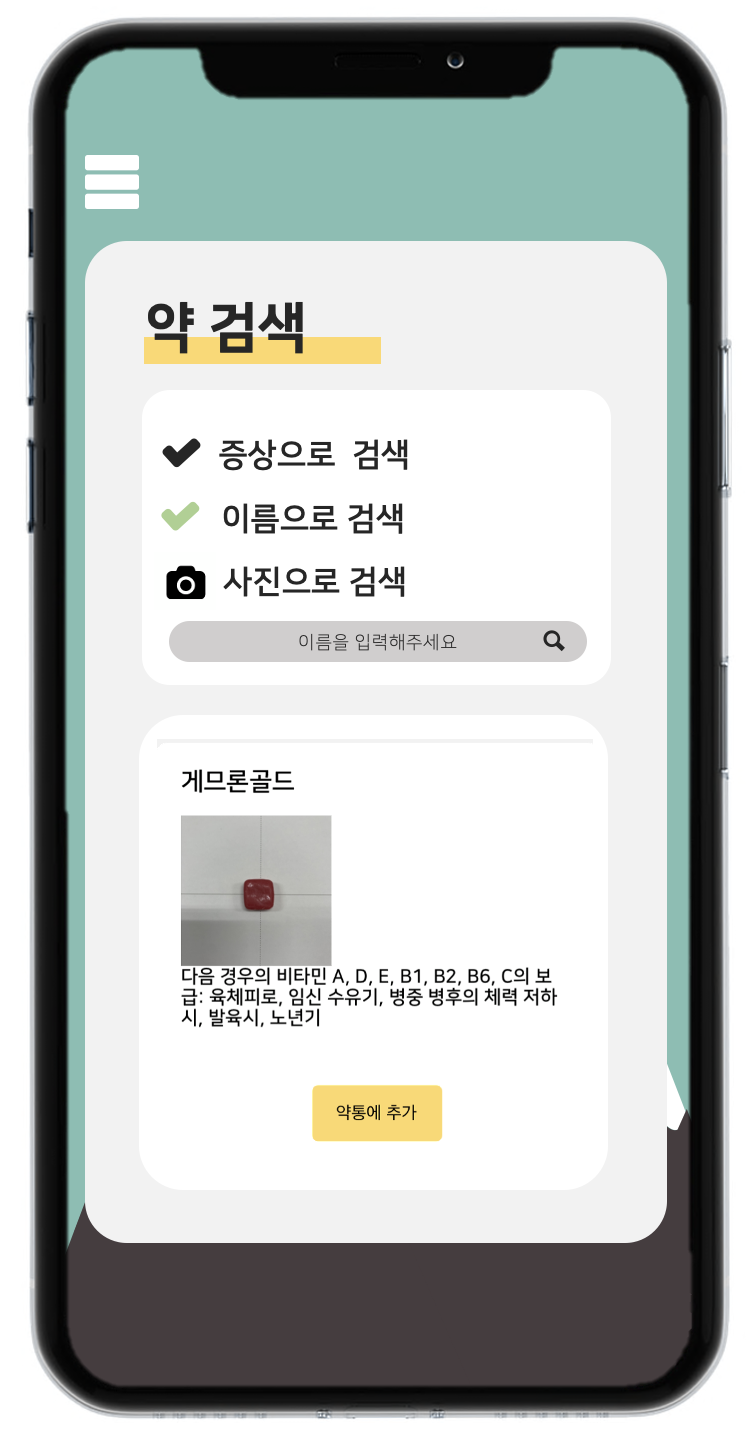
\includegraphics[width=5cm]{final_image_folder/search_result.png}
\caption{}
\label{fig:map}
\end{figure}

\begin{figure}[h!]
\centering
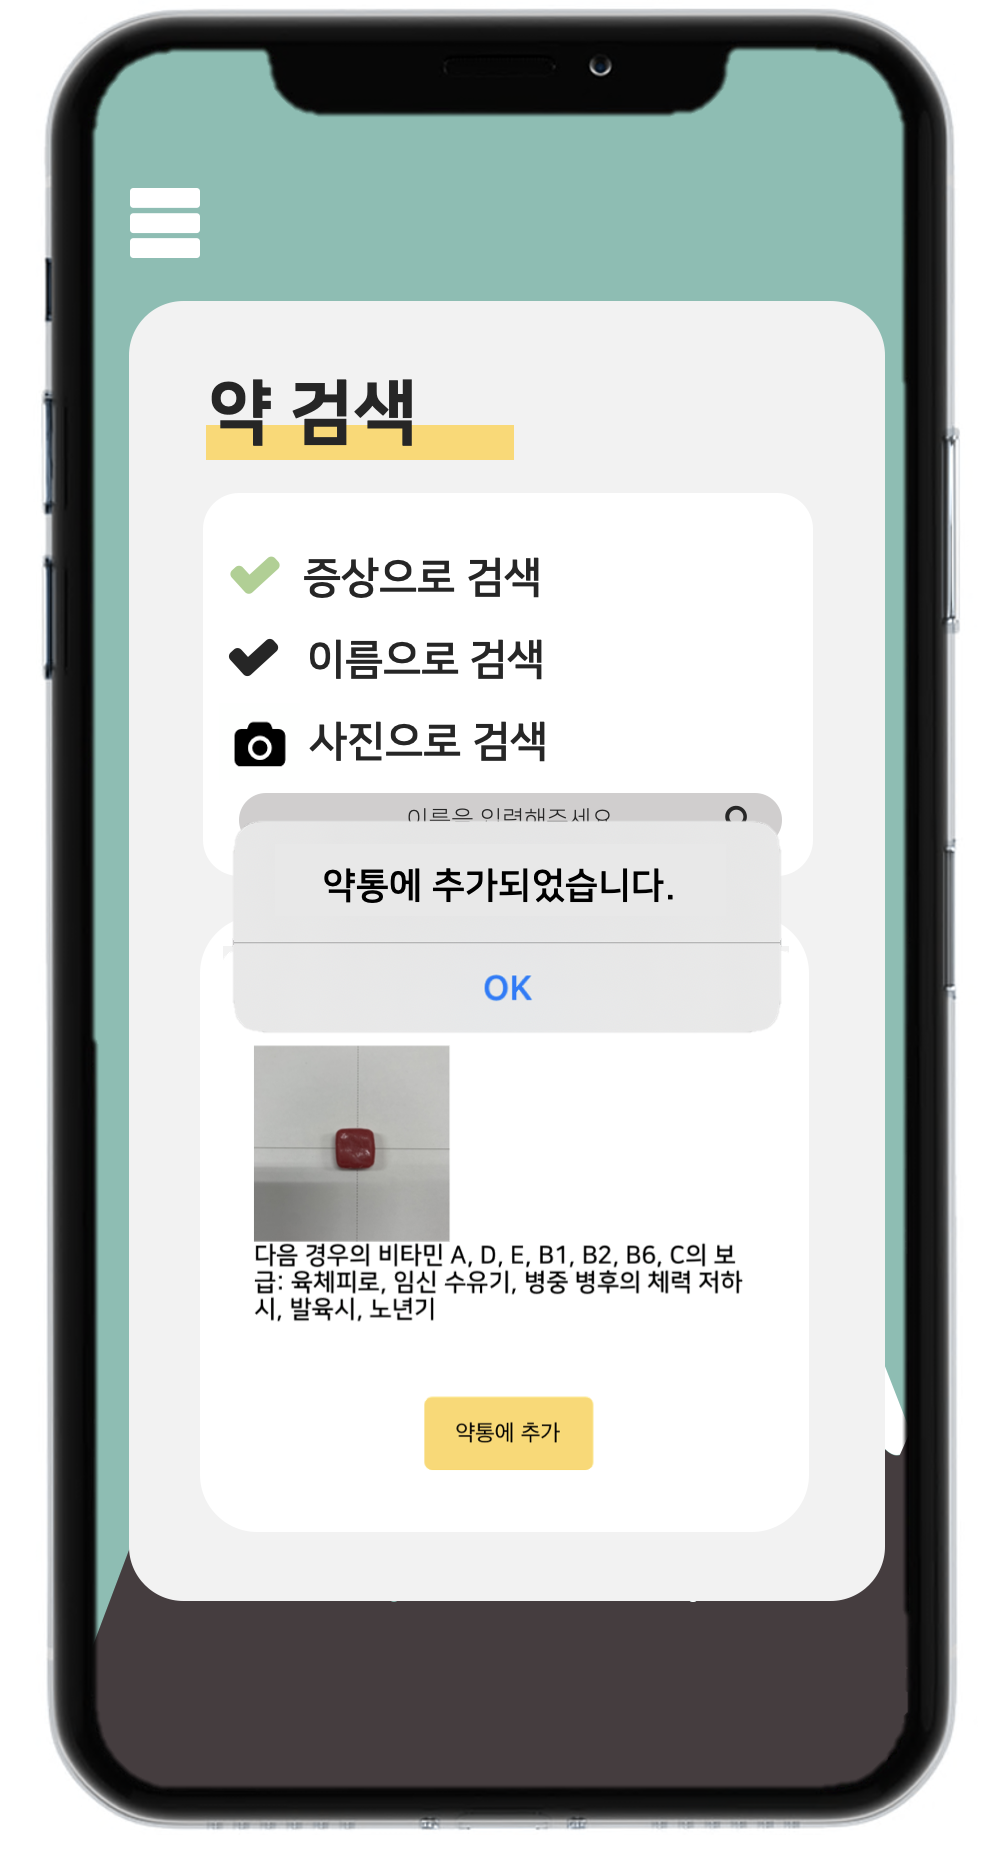
\includegraphics[width=5cm]{final_image_folder/search_add.png}
\caption{}
\label{fig:map}
\end{figure}
.\\
\\

\subsubsection{No Information}
If there is no pill information related to the search keyword or photo, the sentence 'There is no pill you are looking for' appears on the screen.\\

\begin{figure}[h!]
\centering
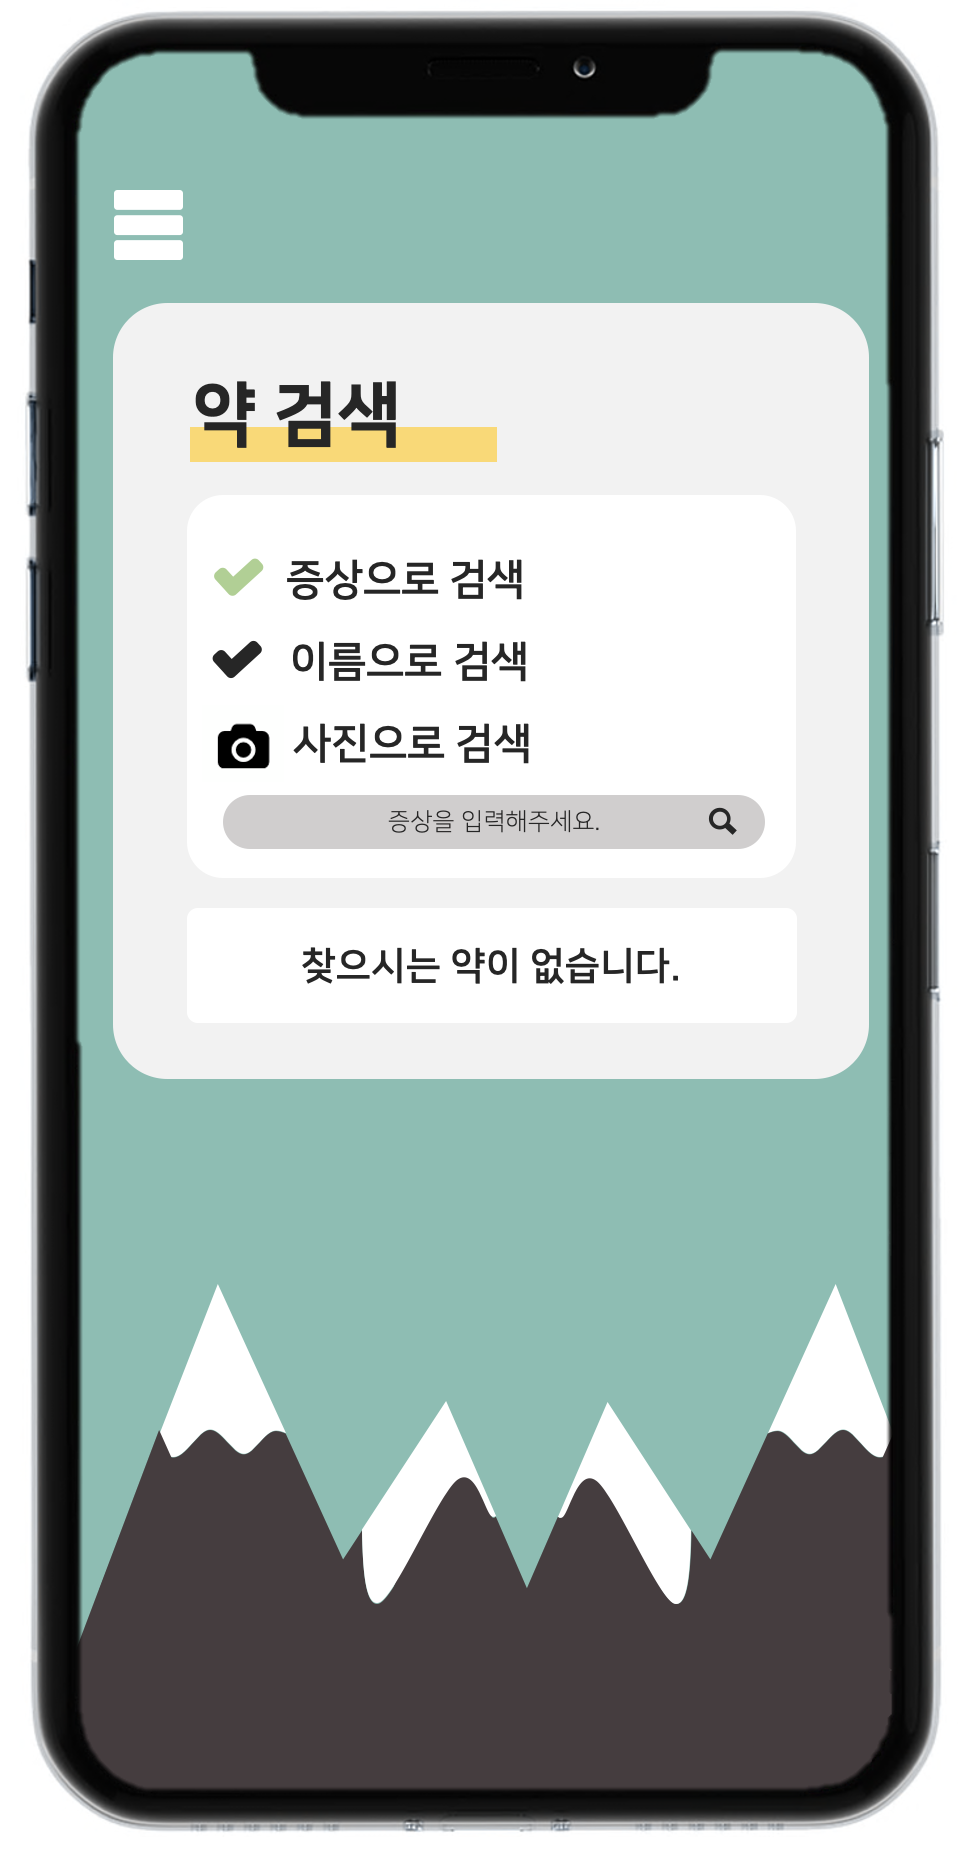
\includegraphics[width=5cm]{final_image_folder/search_noresult.png}
\caption{}
\label{fig:map}
\end{figure}

\subsection{Pill Box}\\

\subsubsection{Pills List}
If the user clicks the add to pill box button after searching for pills, the pills are added to their respective pill boxes. Each pill box has the name of the pill, the shape and color of the pill, and a brief description. Also, each square box has a sign board-shaped mark meaning information and a bell-shaped mark meaning alarm setting.\\

\begin{figure}[h!]
\centering
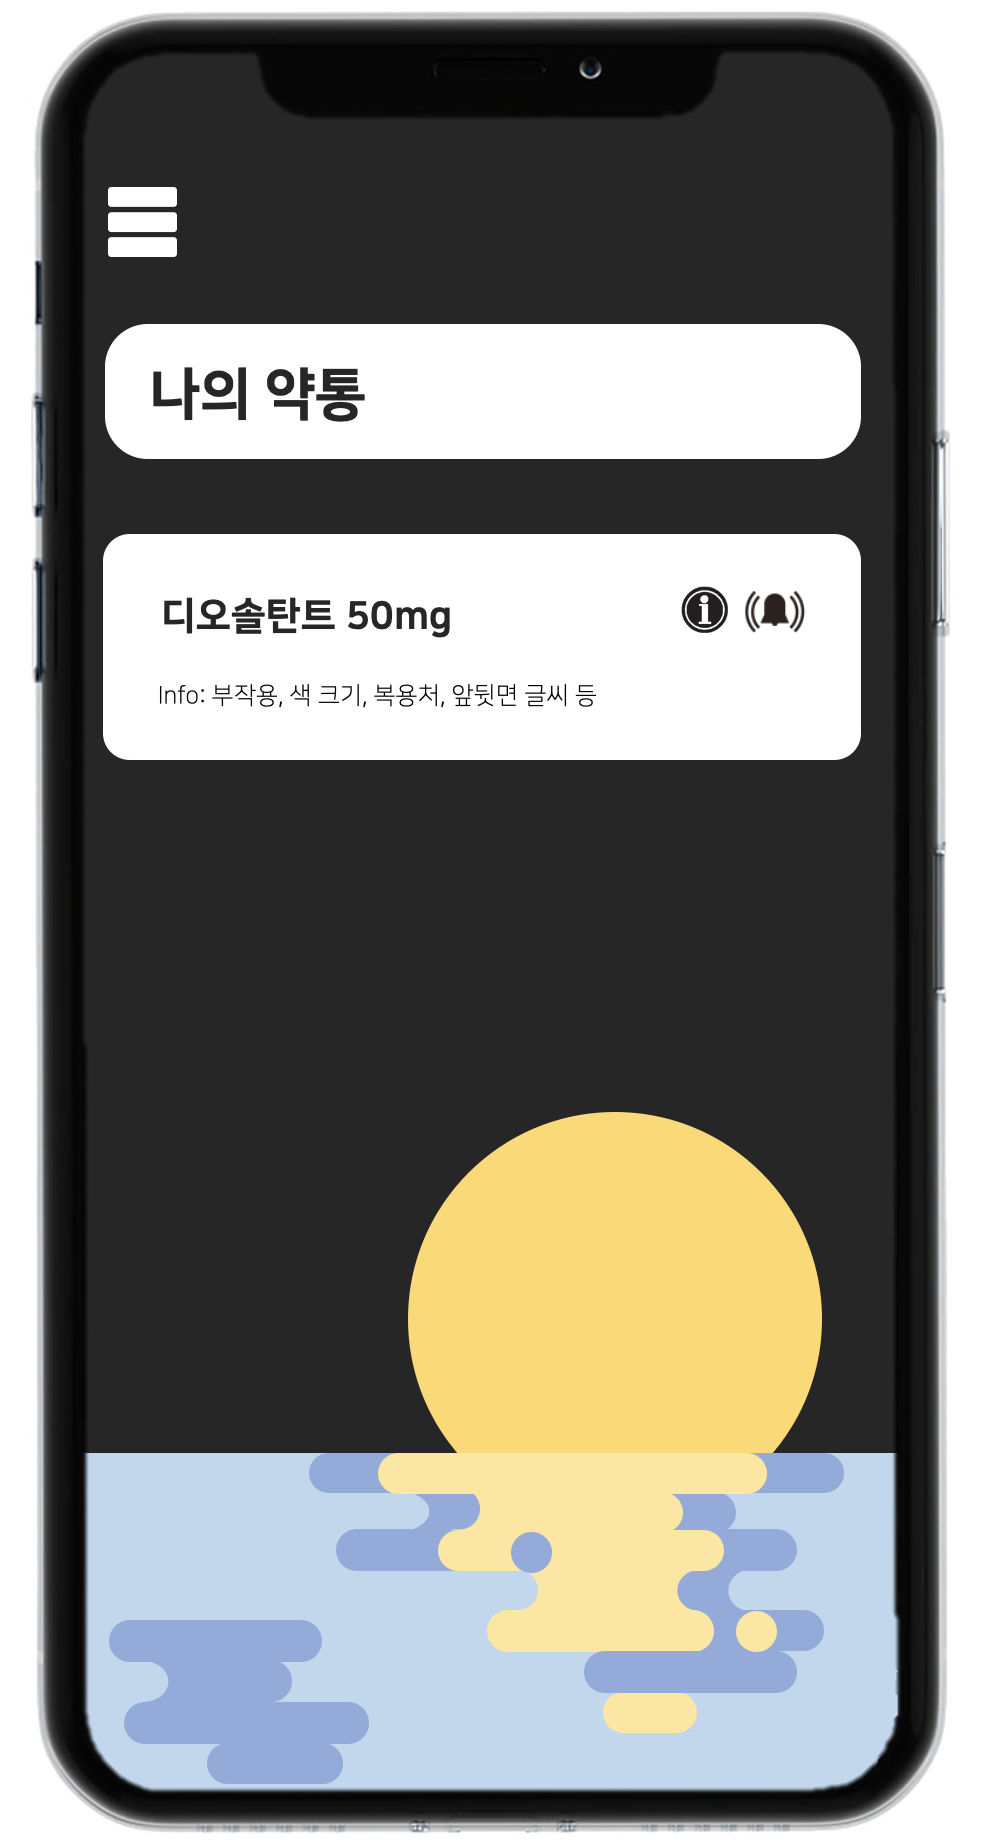
\includegraphics[width=5cm]{final_image_folder/pillbox.png}
\caption{}
\label{fig:map}
\end{figure}
.\\
\\
\\
\\
\\
\\
\\
\\
\\
\\
\\
\\
\\
\\
\\
\\

\subsubsection{Information}
If users click the sign board-shaped first icon in the lower right corner inside each pill box, they can see detailed information about the pill. \\

\begin{figure}[h!]
\centering
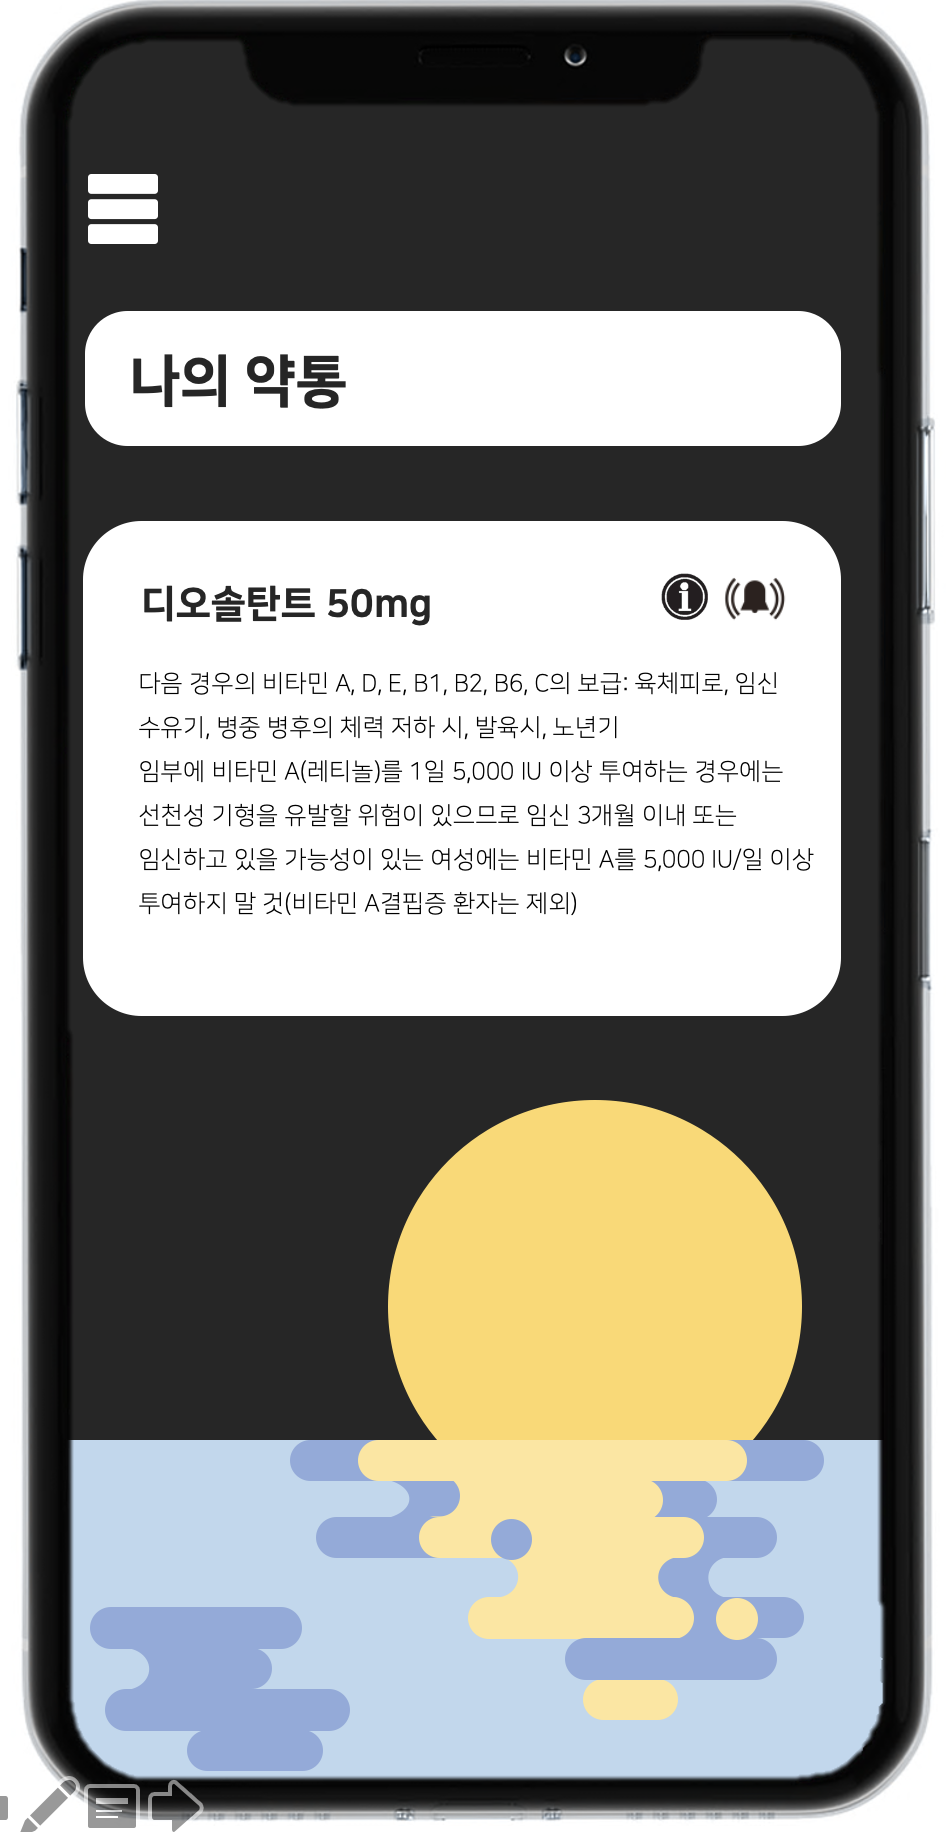
\includegraphics[width=5cm]{final_image_folder/pillbox_info.png}
\caption{}
\label{fig:map}
\end{figure}

\subsubsection{Alarm Setting}
If users click the bell-shaped second icon, they can set the notification for each pill. Users can specify when the pill should be taken in the alarm settings. A new time can be added or deleted. When the user enters the period of taking the pill, an alarm is sent for the corresponding period.\\

\begin{figure}[h!]
\centering
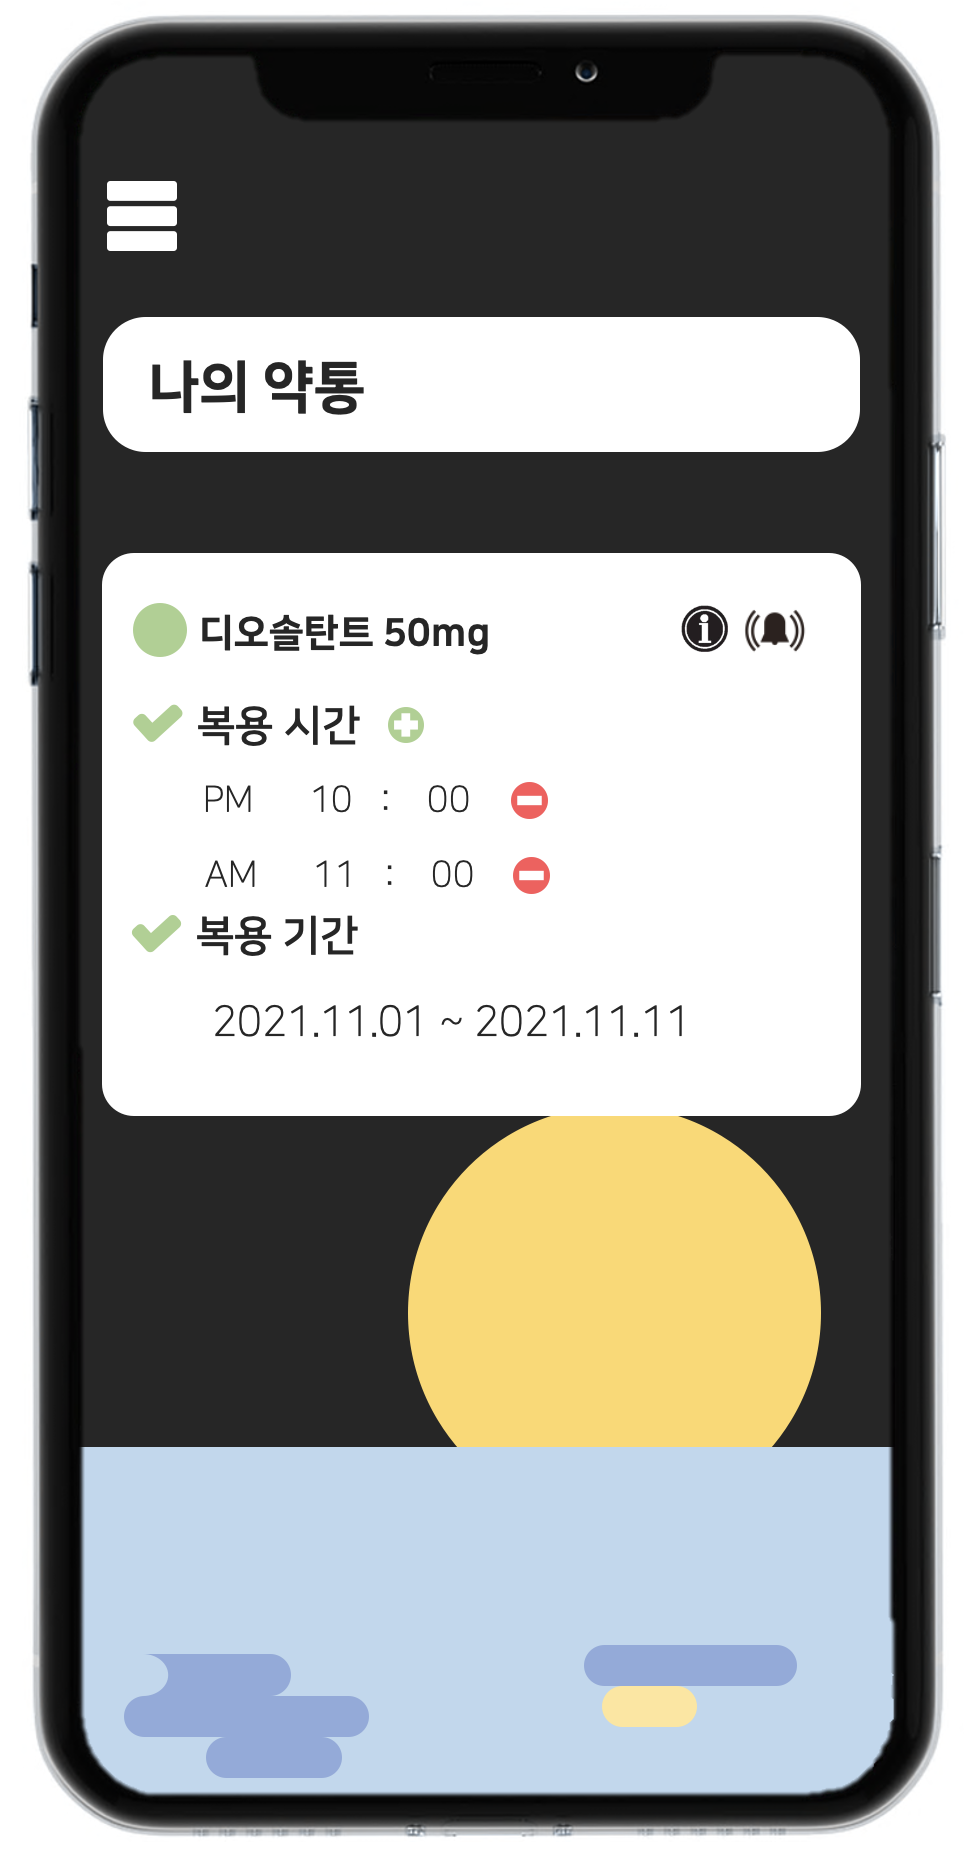
\includegraphics[width=5cm]{final_image_folder/pillbox_alarm.png}
\caption{}
\label{fig:map}
\end{figure}
.\\
\\
\\
\\
\\
\\
\\
\\
\\
\\
\\
\\
\\
\\
\\
\\
\\
\\
\\
\\
\\

\paragraph{Add Alarm}
When users press the + button to add an alarm, the Add Notification popup appears. In the Add Notification pop-up, 'Please enter a new alarm' in large letters and 'Please enter it in the same format as 10:00 AM' in small letters are written. If the user writes down the time in the suggested format and presses OK, the alarm is saved. If the user presses Cancel, it returns to the previous page without saving the alarm.\\

\begin{figure}[h!]
\centering
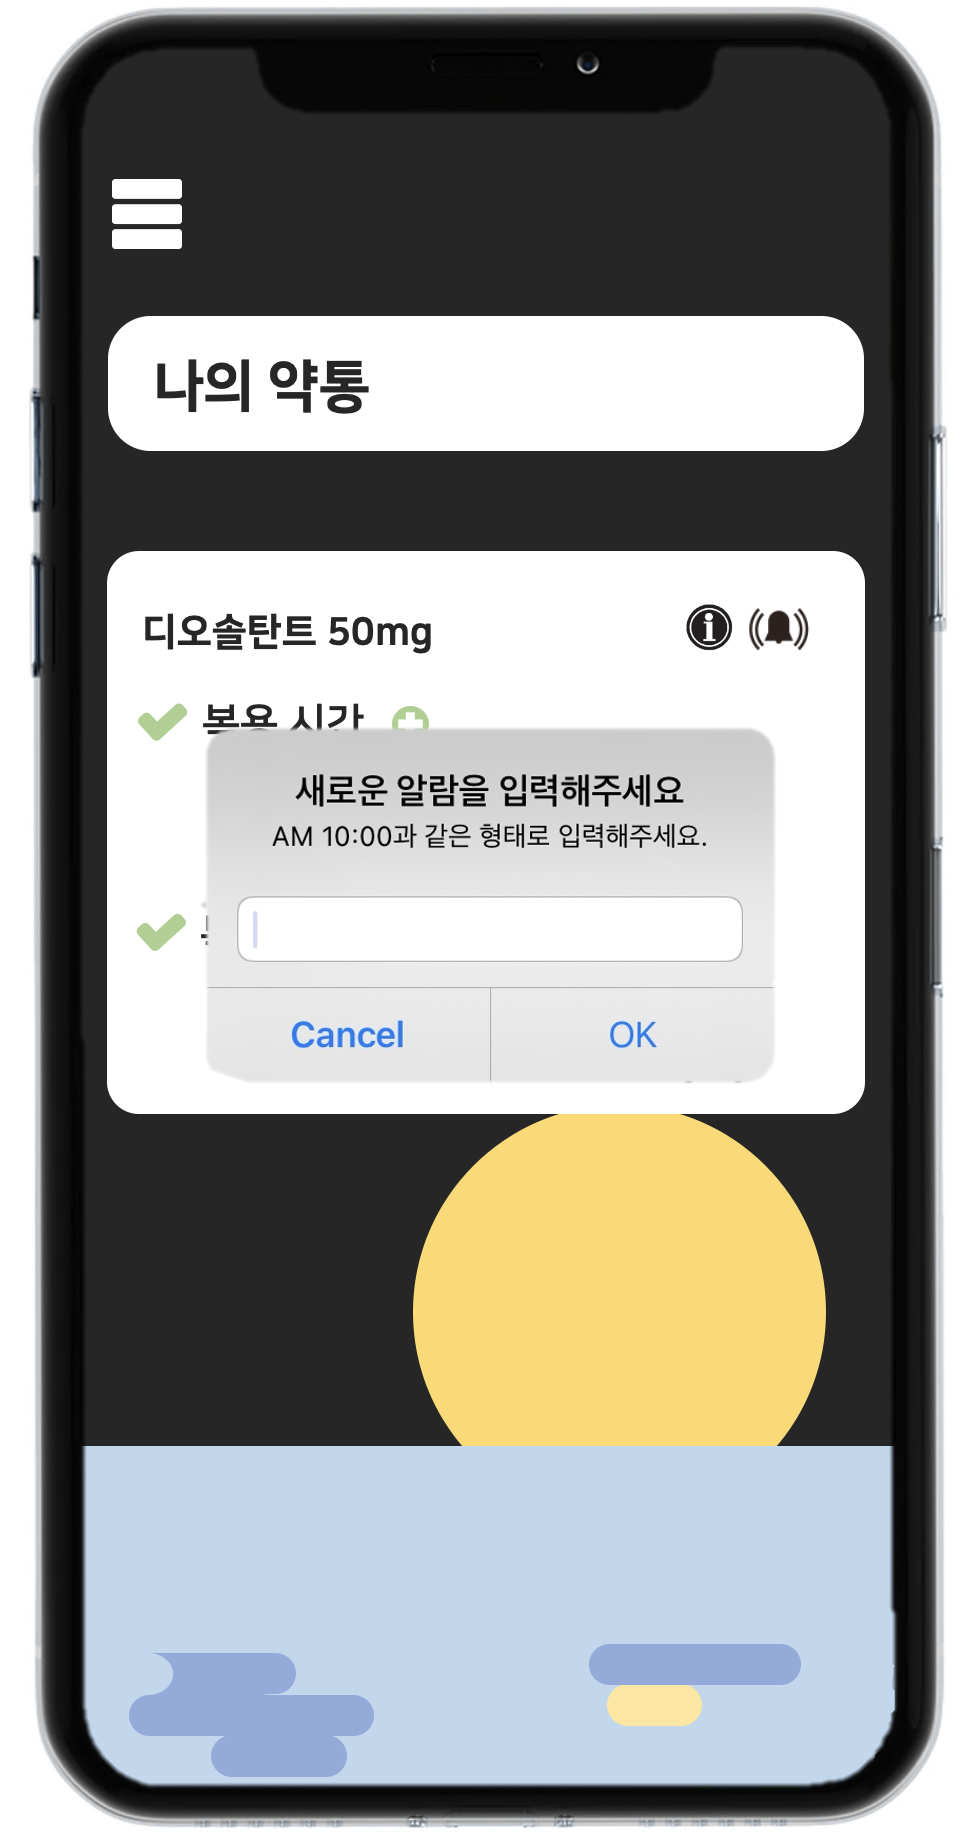
\includegraphics[width=5cm]{final_image_folder/pillbox_alarm_add.png}
\caption{}
\label{fig:map}
\end{figure}
.\\
\\
\\
\\
\\
\\
\\
\\
\\
\\
\\
\\
\\
\\
\\
\\
\\
\\
\\

\paragraph{Delete Alarm}
When users press the - button to delete an alarm, the Delete Notification popup appears. In the Delete Notification pop-up, 'Delete Alarm' in large letters and 'Are you sure you want to delete the alarm?' in small letters are written. If the user clicks 'Yes' in red, the alarm is deleted. If the user clicks the blue 'No', the alarm is not cleared and he or she is returned to the previous page.\\

\begin{figure}[h!]
\centering
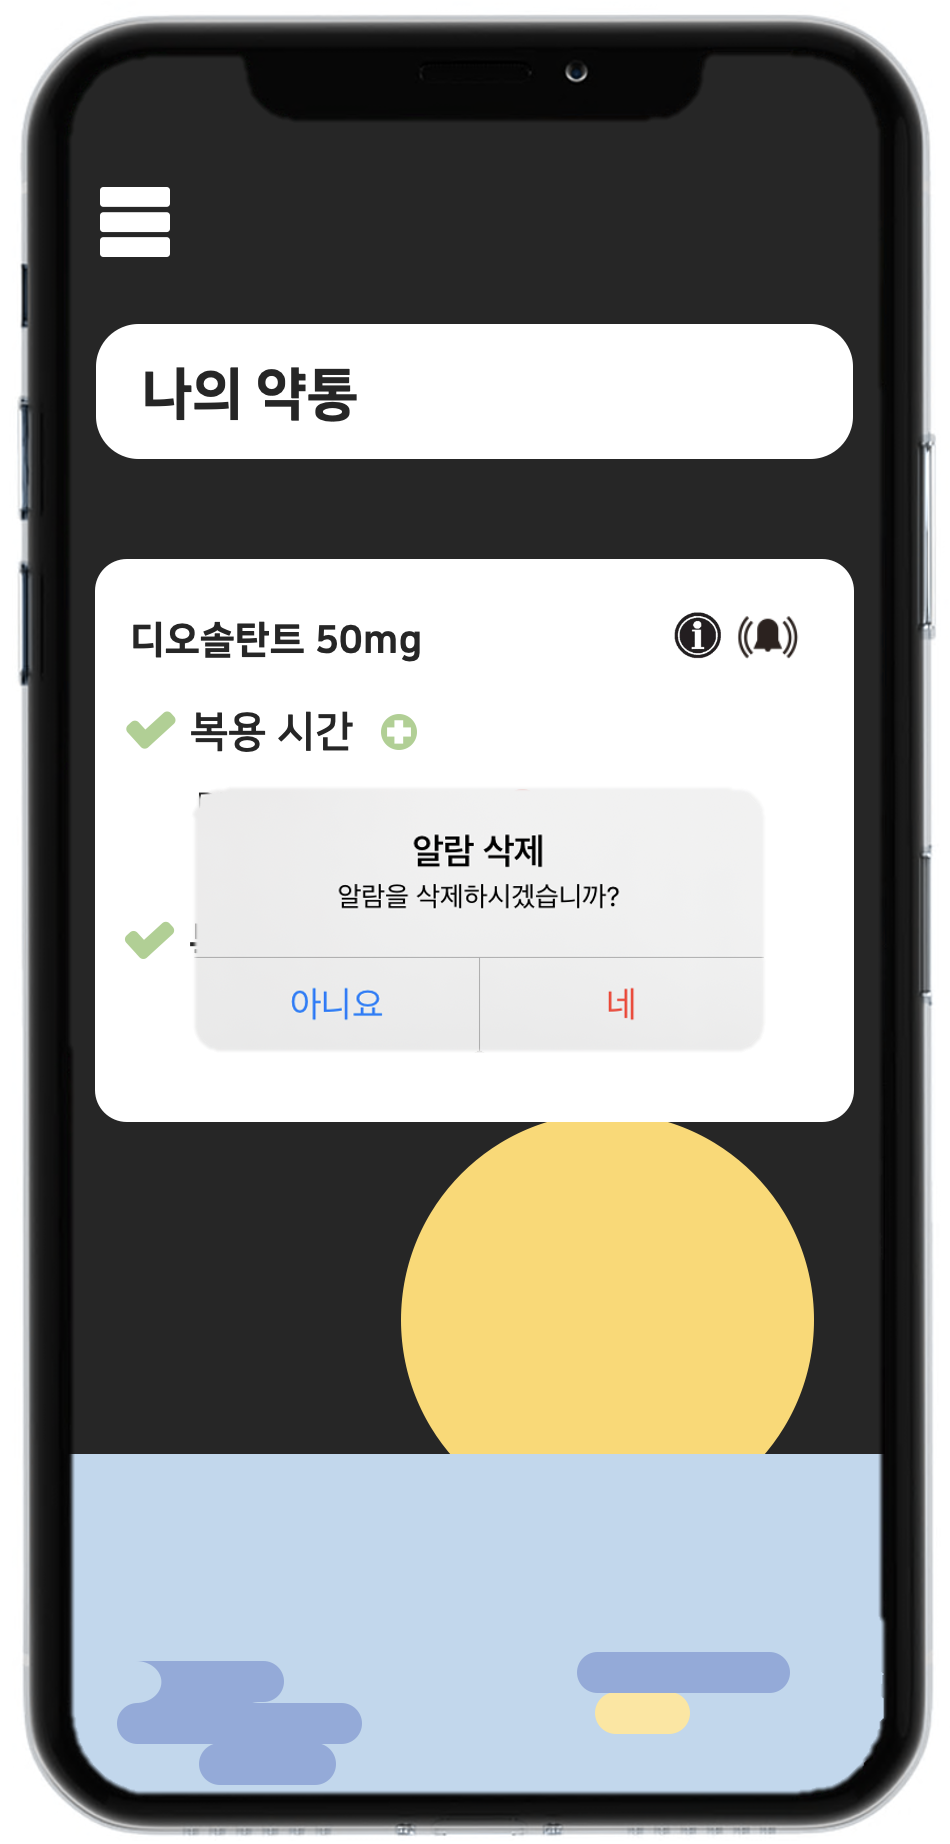
\includegraphics[width=5cm]{final_image_folder/pillbox_alarm_remove.png}
\caption{}
\label{fig:map}
\end{figure}
.\\
\\
\\
\\
\\
\\
\\
\\
\\
\\
\\
\\
\\
\\
\\
\\
\\
\\
\\

\subsection{Today's Pills}
\subsubsection{Before Recognition}
If a user enters today's pill menu, the user can take a picture or upload a picture that they have taken. When a user inputs a photo into the application, the photo goes to the server.\\ 

\begin{figure}[h!]
\centering
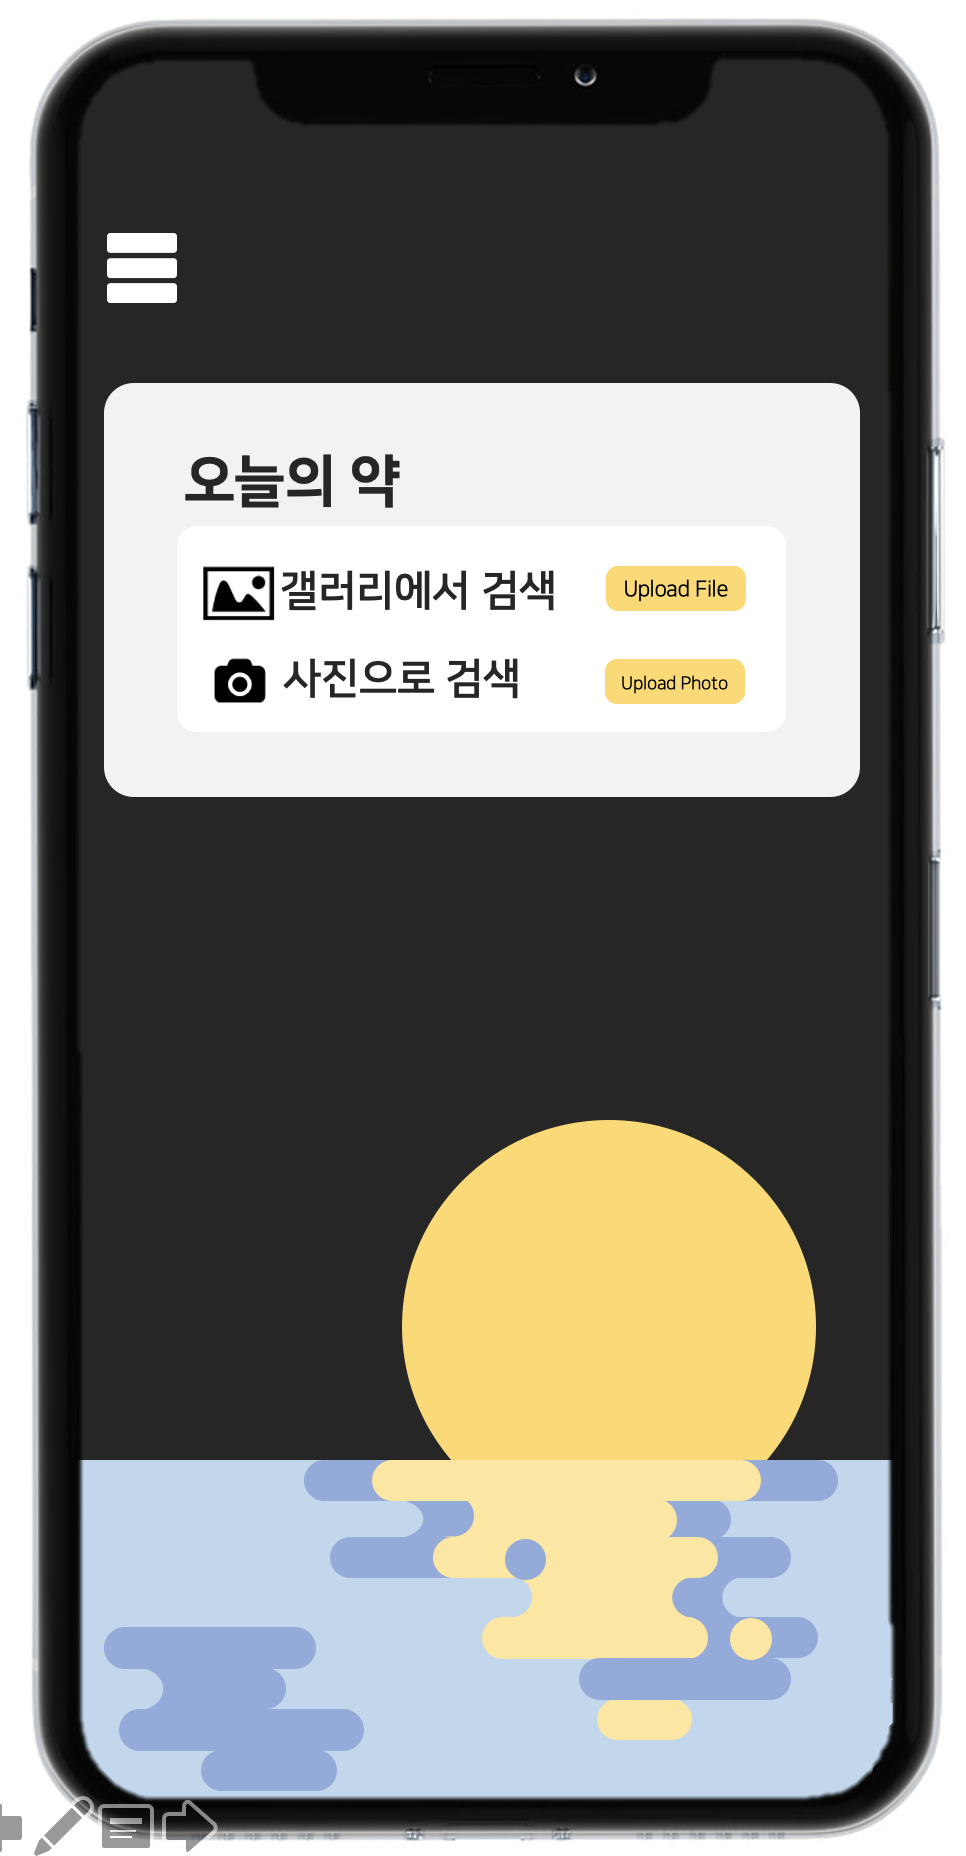
\includegraphics[width=5cm]{final_image_folder/today.png}
\caption{}
\label{fig:map}
\end{figure}
.\\
\\
\\
\\
\\
\\
\\
\\
\\
\\
\\
\\
\\
\\
\\
\\
\\
\\
\\
\\
\\

\subsubsection{After Recognition}
The server finds out which pills each of the pills in the photo are. After that, it sends information whether the pills in the picture are the right pills to take now. \\ 

\paragraph{If yes} If yes, the server sends a notification saying '
You took all the pills well! We will check the reminder.'. \\

\begin{figure}[h!]
\centering
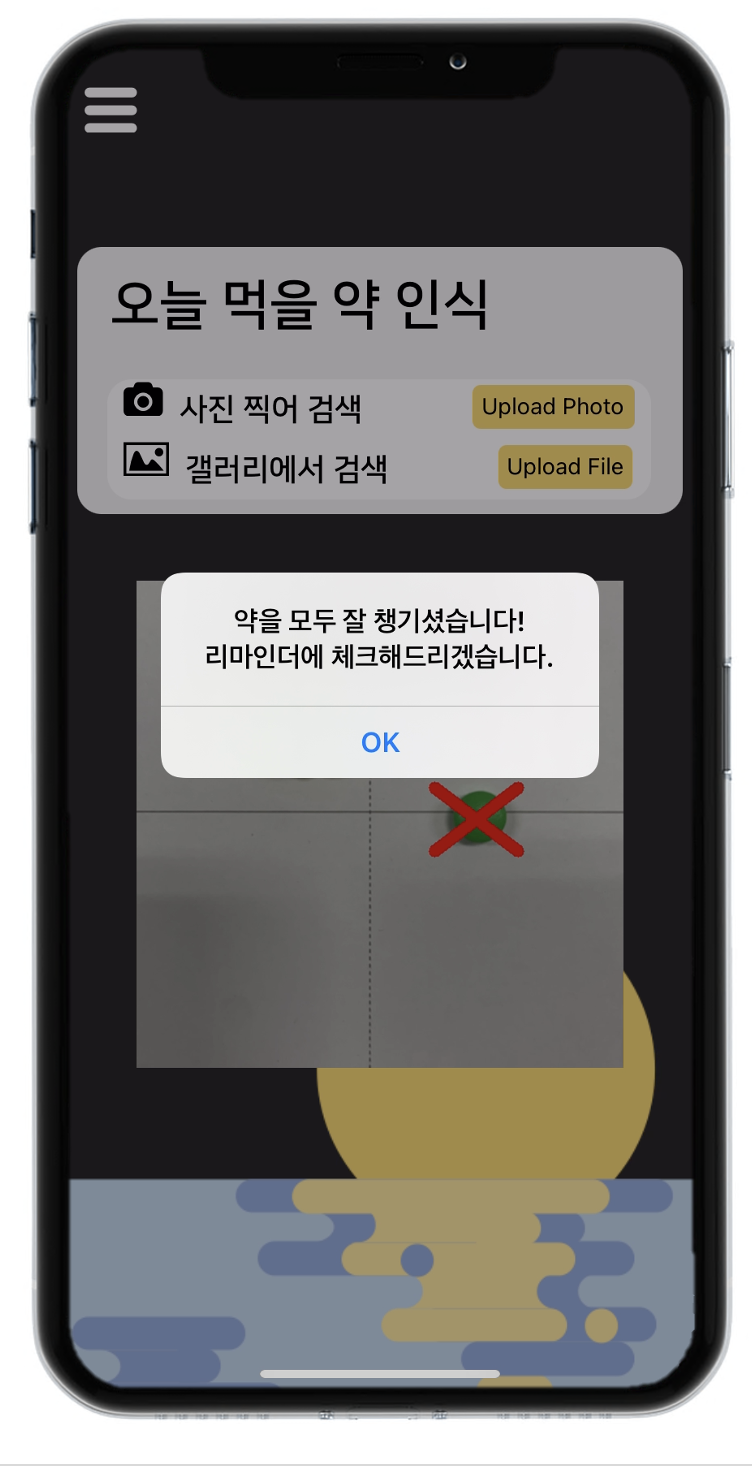
\includegraphics[width=5cm]{final_image_folder/today_result2.png}
\caption{}
\label{fig:map}
\end{figure}
.\\
\\
\\
\\
\\
\\
\\
\\
\\
\\
\\
\\
\\
\\
\\
\\
\\
\\
\\
\\

\paragraph{If no}  Otherwise, the server will sends a pop up that states 'Please take out the N tablets of XX pill.'.\\

\begin{figure}[h!]
\centering
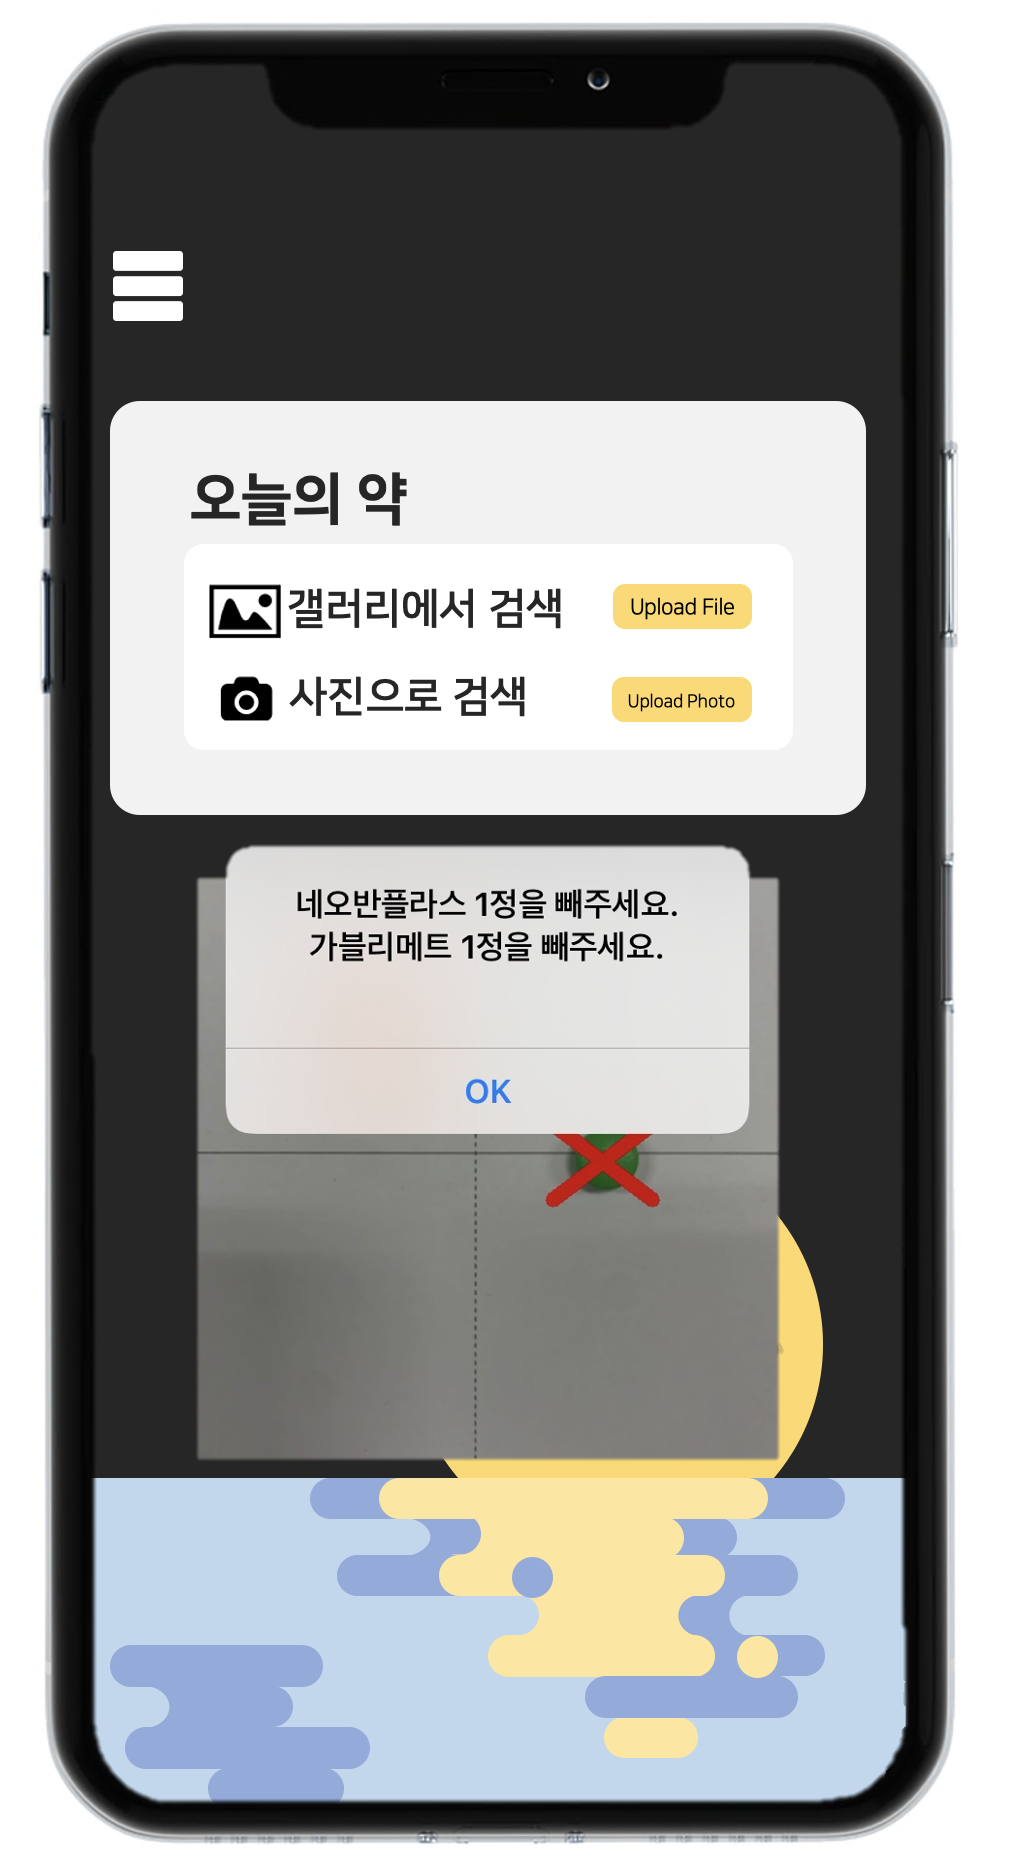
\includegraphics[width=5cm]{final_image_folder/today_result.png}
\caption{}
\label{fig:map}
\end{figure}
.\\
\\
\\
\\
\\
\\
\\
\\
\\
\\
\\
\\
\\
\\
\\
\\
\\
\\
\\
\\
\\
\\
\\
\\
\\
\\

\paragraph{Clicking OK} If the users click OK on the pop up, they can check the photo from server that notify them if the pills are correct or not. If one pill is the right pill the user should take now, a green check mark will appear over the pill. If not, a red X will appear over the pill. The indications are large and intuitive, easy to recognize. \\

\begin{figure}[h!]
\centering
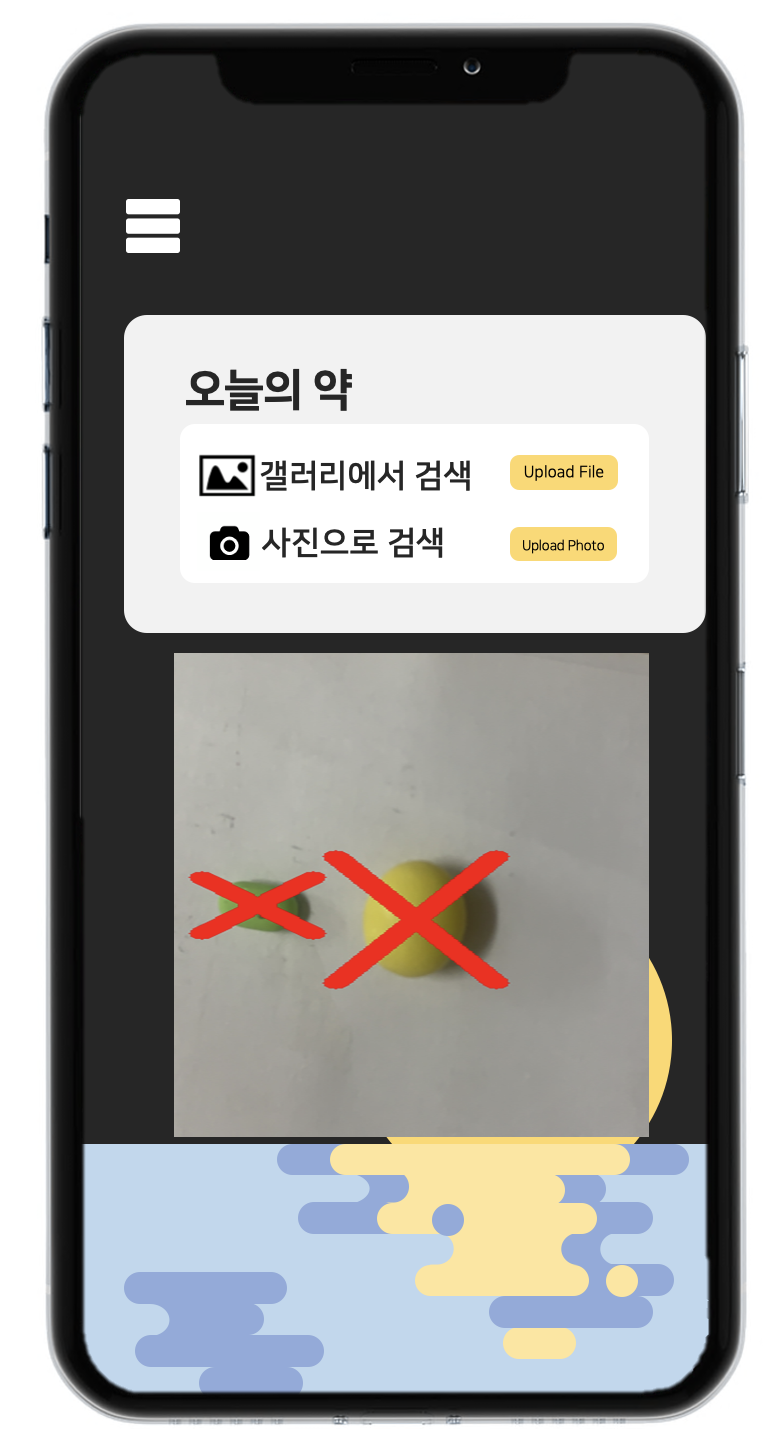
\includegraphics[width=5cm]{final_image_folder/today_result_photo.png}
\caption{}
\label{fig:map}
\end{figure}

\subsection{Caregiver Links}

\paragraph{Search Caregivers}
Wards can search the names of caregivers.\\

\subparagraph{1.If the name is in DB: }
If the name they entered into the search bar is in the server's DB, users associated with that name will be listed.\\

\begin{figure}[h!]
\centering
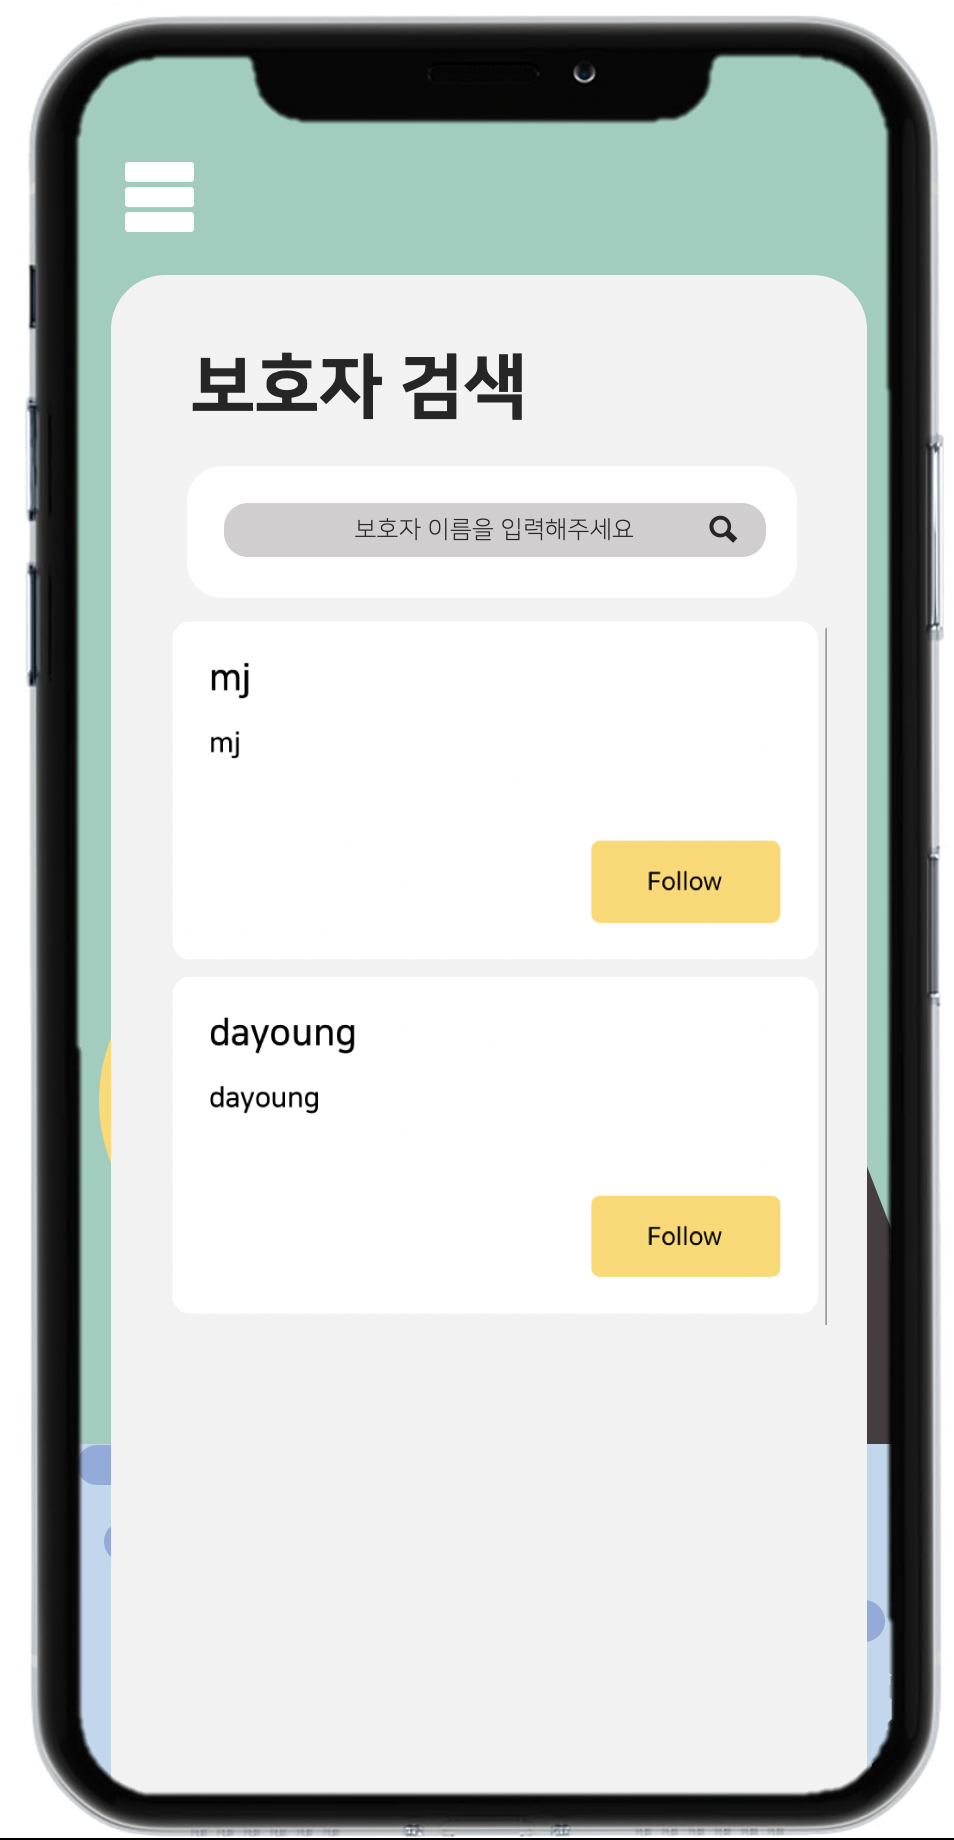
\includegraphics[width=5cm]{final_image_folder/bohoja_result.png}
\caption{}
\label{fig:map}
\end{figure}
.\\
\\
\\
\\
\\
\\
\\
\\
\\
\\
\\
\\
\\

\subparagraph{2. If the name isn't in DB: }
If the name they entered is not in the server's DB, the sentence 'There is no guardian you are looking for' appears.\\

\begin{figure}[h!]
\centering
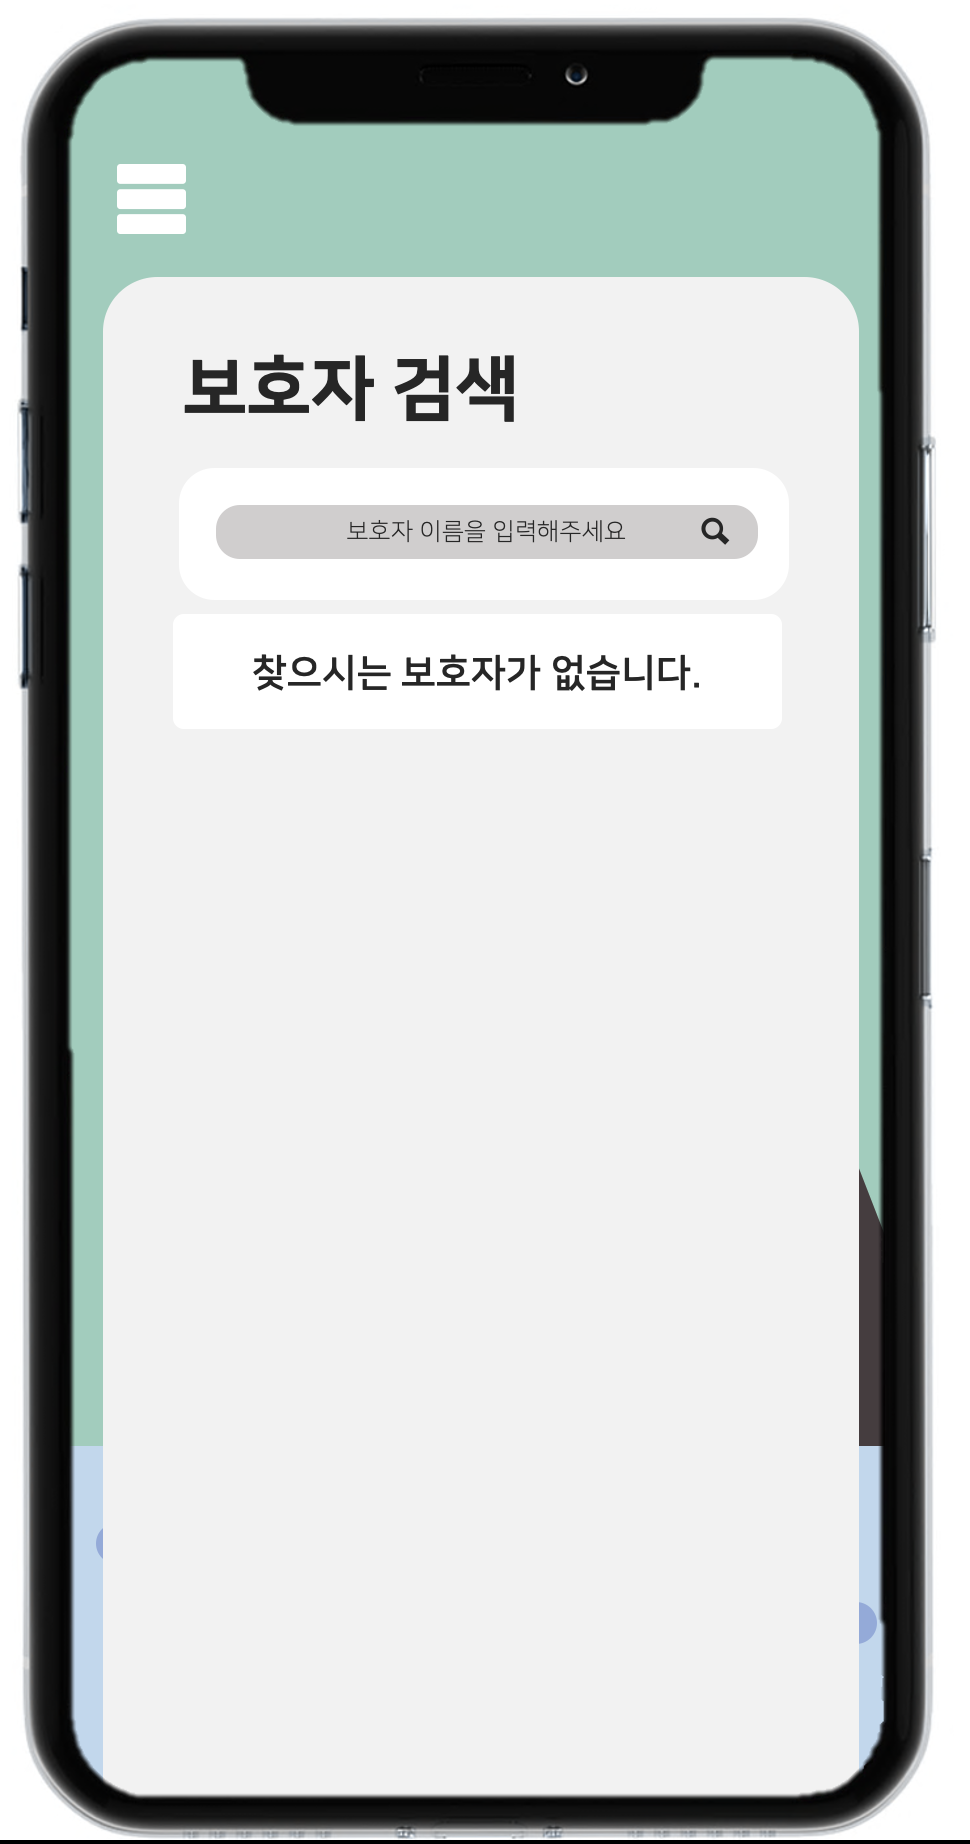
\includegraphics[width=5cm]{final_image_folder/bohoja_noresult.png}
\caption{}
\label{fig:map}
\end{figure}

\paragraph{Follow Caregivers}
Wards can follow their caregivers by clicking yellow follow button. After that, server will send a notification that says 'Your follow request has been processed.'.caregivers can manage the pill list of the wards followed them. In this way, they can check whether their wards are taking the pill well.\\

\begin{figure}[h!]
\centering
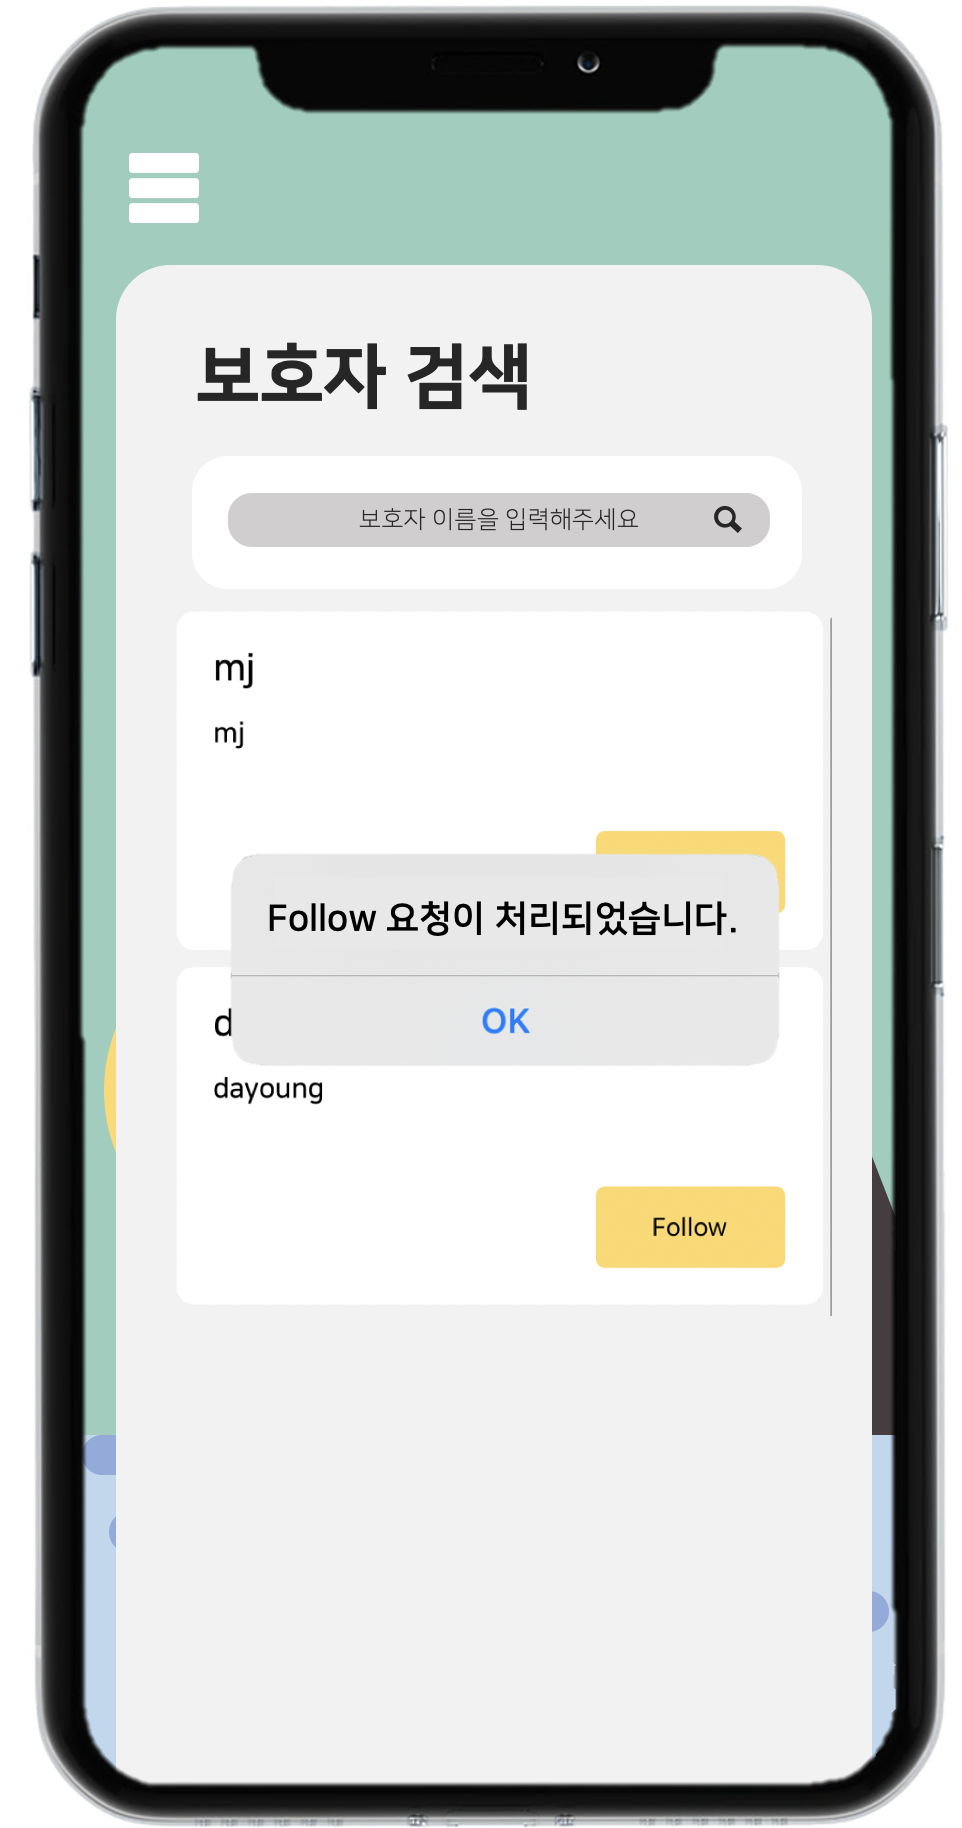
\includegraphics[width=5cm]{final_image_folder/bohoja_follow.png}
\caption{}
\label{fig:map}
\end{figure}

\subsection{NUGU INTERFACE}
The user can user the custom Nugu play for the PharmaSEE mobile application. The Nugu interface can be invoked by using the invocation keyword 'PharmaSEE'. Once invoked, the user can ask about the intake status to the Nugu interface. \\ \\
The questions will be interpreted by the Nugu device into 'intents' and sent to the backend proxy server we have developed. Each 'intent' will be mapped to a specific 'action'. The Nugu device will send requests to the url which will be defined as 'BASE\_URL + action name'. In exapmle, is the intent 'ask.taken\_pills' is requested, the request url will be 'http://host:port/nugu/answer.taken\_pills'. This request will invoke a function that will read information from the Reminder table in the database. The information will be woven together and structured into a string that contains data about the user's intake history. \\ \\
The architecture can be understood with this diagram below. User utterance is interpreted by the Nugu device into intents such as ask.taken\_pills, and the backend proxy will response with the corresponding action, which in this case is answer.taken\_pills. The response will be prompted to the user through the Nugu device.

\begin{figure}[h!]
\centering
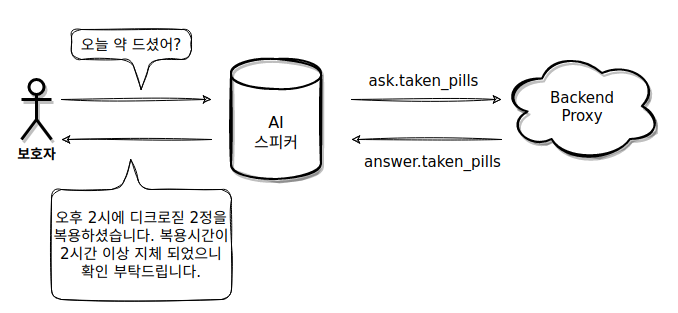
\includegraphics[width=5cm]{final_image_folder/nugu_arch.png}
\caption{}
\label{fig:map}
\end{figure}

\begin{itemize}%[leftmargin=1em]
  \renewcommand{\labelitemi}{$\rightarrow$}
 \item User’s Voice Command \\
 
 \item Intent Extracted by NUGU\\
 
 \item Parameters Sent to Backend Proxy\\
 
 \item REST API Response Processed by Backend Proxy\\
 
 \item Respond in Voice Through NUGU\\
\end{itemize}

\begin{table}[h!]
\begin{tabular}{|p{0.135\textwidth}|p{0.13\textwidth}|p{0.16\textwidth}|}
\cline{1-3} 
\textbf{Intent/Action} &\textbf{User Utterance} & \textbf{Response}\\
\hline
ask.taken\_pills \newline answer.taken\_pills&오늘 먹은 약 뭐야?&오후 4시에 게므론골드 2정, 디크로짇 1정을 복용하셨습니다. 복용 예정 시간에서 2시간 이상 지체하여 복용한 약이 있으니 주의 부탁드립니다. \\
\hline
ask.not\_taken\_pills \newline answer.not\_taken\_pills&오늘 까먹은 약 있어?&오후 1시에 예정된 디크로짇 1정을 아직 복용하지 않으셨습니다. 확인 부탁드립니다. 오후 9시에 셀카토린 1정을 복용할 예정입니다.\\
\hline
ask.total\_status \newline answer.total\_status&오늘 약 먹었어/드셨어?&오전 9시에 디크로짇 1정을 복용하셨습니다. 오후 1시에 예정된 디크로짇 1정을 아직 복용하지 않으셨습니다. 확인 부탁드립니다. 오후 9시에 셀카토린 1정을 복용할 예정입니다.\\
\hline
\end{tabular}
\label{tab1e}
\end{table}

\paragraph{Ask Taken Pills}
Users can ask the Nugu device questions such as 'What pills did I take today?'. These expected user utterances are grouped to have the intent of asking the pills taken today. In the Nugu play builder, these user utterances are defined as the intent 'ask.taken\_pills'. \\ \\
The Nugu player will interpret all related user utterances to have this intent and invoke the corresponding action 'answer.taken\_pills'. This action will invoke a view function in the backend proxy. \\ \\
When the backend proxy is requested to process this action, it will go through the following steps to formulate an adequate response.
\begin{itemize}
    \item Import the Reminder model\\
    \item Make a query set from the Reminder model, consisting of the entries that match the user who is requesting\\
    \item Filter the Reminder query set to contain only the entries that are checked as 'taken\_today'\\
    \item Iterate through each Reminder object in the query set and read information such as the pill name, the dose that has been took, the time of intake, etc.\\
    \item Formulate those information into a string. (ie. You(He/She in the case the user is the caretaker) took 2 doses of Dicroix at 9AM today.)\\
    \item The when\_to\_take field, which contains the time the user has selected as the appropriate time to take the medicine, will be compared with the actual time taken. If they differ by more than 2 hours, a warning message will be added to the prompt. (ie. This is 2 hours later than the expected time, so please take caution.)\\
    \item The entries will be grouped by time and formulated into a prompt string. Therefore if there are several entries that were taken at the same time, they will be read to the user in the following manner. "You took 1 dose of Dicroix, 2 doses of Tylenol at 9AM."\\
\end{itemize}

\paragraph{Ask Not Taken Pills}
Users can ask the Nugu device questions such as 'What pills did I forget today?'. These expected user utterances are grouped to have the intent of asking the pills the user forgot to take today, or has to take at a later time that day. In the Nugu play builder, these user utterances are defined as the intent 'ask.not\_taken\_pills'. \\ \\
The Nugu player will interpret all related user utterances to have this intent and invoke the corresponding action 'answer.not\_taken\_pills'. This action will invoke a view function in the backend proxy. \\ \\
When the backend proxy is requested to process this action, it will go through the following steps to formulate an adequate response.
\begin{itemize}
    \item Import the Reminder model\\
    \item Make a query set from the Reminder model, consisting of the entries that match the user who is requesting\\
    \item Filter the Reminder query set to contain only the entries that are checked as 'not\_taken\_today'\\
    \item Iterate through each Reminder object in the query set and read information such as the pill name, the dose that has to be taken, the time it is scheduled at.\\
    \item Formulate those information into a string. The string will be formulated differently for cases in which the pill intake is overdue, and when the pill intake is scheduled in the future. (ie. You(He/She in the case the user is the caretaker) forgot to take one dose of Dicroix at 7pm today. You are scheduled to take 2 doses of vitamins later at 9pm.)\\
\end{itemize}

\noindent
\newpage

\section{Architecture Design And Implementation}
\subsection{Overall Architecture}

The PharmaSEE project is an mobile application with the front-end client and back-end server managing the database. The front received server information using React Native's fetch function. In the Get method, information has been received, and in the Post method, information is sent to the server and a response is received. Below is a diagram visualizing the relation.

\begin{figure}[h!]
\centering
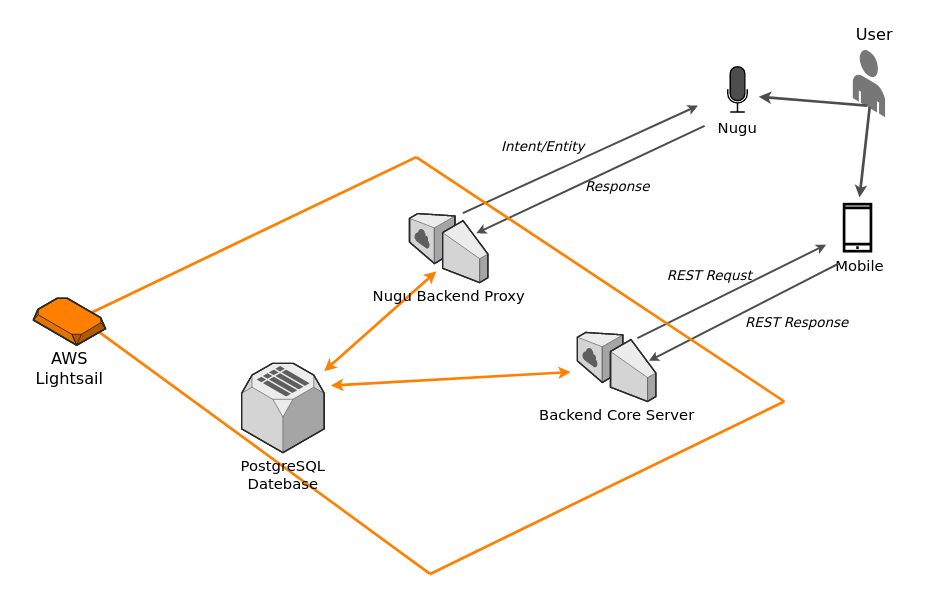
\includegraphics[width=0.5\textwidth,height=0.25\textheight]{imagefolder/arch.png}
\caption{}
\label{fig:map}
\end{figure}

\subsection{Directory Organization}
\noindent
\newpage
\par \begin{table}[h!]
\begin{tabular}{|p{0.1\textwidth}|p{0.15\textwidth}|p{0.1\textwidth}|}
\cline{1-3} 
\textbf{Directory} & \textbf{\textit{File Name}}& \textbf{\textit{Module Name}}\\
\hline
Server/backend/ backend &settings/common.py \newline\newline settings/dev.py \newline\newline settings/prod.py \newline\newline urls.py wsgi.py&Django - backend\\
\hline
Server/backend/ accounts &models.py \newline\newline urls.py \newline\newline views.py \newline\newline serializers.py \newline\newline forms.py \newline\newline apps.py \newline\newline admin.py \newline\newline migrations/ \newline\newline templates/accounts/signup  \_form.html&Django - accounts\\
\hline
Server/backend/ pharmasee &models.py \newline\newline urls.py \newline\newline views.py \newline\newline serializers.py \newline\newline apps.py \newline\newline admin.py \newline\newline migrations/ &Django - pharmasee\\
\hline
Server/backend/ nugu &urls.py \newline\newline views.py&Django - nugu\\
\hline
Server/backend/ pill\_ai &models.py \newline\newline serializers.py \newline\newline views.py \newline\newline urls.py&Django - pill\_ai\\
\hline
Client &CustomSidebarMenu.js \newline\newline App.js \newline\newline App.json \newline\newline style.js &React Native \\
\hline
Client/pages &MainPage.js \newline\newline FindPage.js \newline\newline TodayPage.js \newline\newline PillcasePage.js \newline\newline BohojaPage.js &React Native \\
\hline
Ai\_recognition &  object\_detection.py \newline\newline generate\_tfrecord.py  \newline\newline xml\_to\_csv.py  \newline\newline pills\_ml.py & Tensorflow \\
\hline
Documentation&pharmasee\_doc.tex&Documentation\\
\hline
\end{tabular}
\label{tab1}
\end{table}

\subsection{Module 1 : Django - backend}
\subsubsection{Purpose}
We chose Django to implement our backend server because of its flexibility and many modules provided by it that is useful for building REST apis. In the PharmaSEE project architecture, the Django backend framework has two types of clients to server. The first type of client is the React Native instance that is used for rendering a mobile app interface in the frontend. The second type of client is the Nugu devices that are used by the mobile app users. The mobile app and Nugu device has to be synchronized through the backend server. All requests from external clients will be processed through the Django Backend server with Django Rest Framework. Sychronization between the Nugu devie and mobile application will be done by the tocken suthorizatoin methods that are also built in through Django. CORS settings can be also configured through native Django settings, making the development process much easier and compact.
\\
\subsubsection{Functionality}
\begin{itemize}
    \item Django Rest Framework is a module provided by the django framework. It allows developers to warp their view functions into api endpoints. Requests sent from the frontend mobile application and Nugu devices will be delivered to their endpoint functions wrapped with the Django Rest Framework. Json responses will be rendered out once the requests are properly processed in their according view functions.
    \item Django ORM allows us to connect with the ProstgreSQL database without having to change the source code. ORM(object relational mapping) allows us to programmatically without having to use direct SQL commands.
    \item JSON Web Token Authentication
\end{itemize}

\subsubsection{Location of Source Code}
PharmaSEE/Server/
\\
\subsubsection{Class Component}
\\
\paragraph{backend}
backend application contains basic files necessary for service distribution such as 'settings.py', 'urls.py','wsgi.py','asgi.py'. 
\paragraph{accounts}
accounts application contains basic files necessary for account function. 
\paragraph{pharmasee}
pharmasee application contains basic files necessary for service of managing pills for user.
\paragraph{nugu}
nugu application contains basic files neccessary for service of networking Nugu devices with server. 
\paragraph{pill\_ai}
pill\_ai application contains basic files necessary for service of processing AI work for pills data.  
\\
\subsection{Module 2 : Django - accounts}
\subsubsection{Purpose}
This module is for creating users who use our application 'Pharmasee'. Accounts' database has user's name, first name, second name, email, or whether the caregiver follow each other. And this module provides signup function. Our pharmasee application provides caregiver monitoring system. So accounts module provides follow, unfollow function for monitoring system. Finally, this module provides search function for searching people who need caregiver's help.\\
\subsubsection{Functionality}
\begin{itemize}
    \item Serves to API endpoint /accounts/signup/ 
    \item Serves to API endpoint /accounts/follow/
    \item Serves to API endpoint /accounts/unfollow/
    \item Serves to API endpoint /accounts/search/
\end{itemize}
\bigskip
\subsubsection{Location of Source Code}PharmaSEE/Server/backend/accounts \\
\subsubsection{Class Component}\\
\paragraph{accounts/admin.py}
This file is for administrating account's models on the admin web page. Model manager can create, read, update, delete data on the admin web page. Model manager can check whether data is validate. 
\paragraph{accounts/models.py}
This file is for administrating account's data. We can manage application's data with database. To query database, we use SQL. But by using django model, we can query database without using complex sql. Django model uses ORM(Object-relational mapping) for creating and running sql. Django model and database are connected by one-and-one mapping method. So accounts/models.py's role is connecting with accounts database. accounts/models.py has username, first, last name, email, follower-set, following-set and so on. 
\paragraph{accounts/serializers.py}
Serializers are used for converting complex data to python data. This python data can be converted to JSON or XML. JSON or XML are used in REST API work. And serializer also performs data validation. \\
accounts/serializers.py has two serializers, SignupSerializer and UserSerializer. SignupSerializer serializes signup data. UserSerializer serializers user data. 
\paragraph{accounts/urls.py}
This file defines the url paths for responsing front-end's request. "accounts/signup/" url requests 'user login' data. "accounts/follow" url requests user\_follow data. "accounts/unfollow" url requests user\_unfollow data. "acccounts/search/" url requests user\_searchlist data.
\paragraph{accounts/views.py}
Django view's role is make process of data. accounts/views.py has SignupView, user\_follow, user\_unfollow functions, UserListView. 


\subsection{Module 3 : Django - pharmasee}\\
\subsubsection{Purpose}This module is for managing pill and reminder data. Pharmasee.Pill model's database has pill's name, image\_dir, effect, side\_effect. Pharmasee.Reminder model's database has reminder's title, user\_id, pill\_id, dose, when\_to\_take, taken\_time, is\_taken\_today, dose\_taken\_today. The application uses these data to remind taking pills. From these models serializer can serialize data and convert to JSON datatype. It can make connection between backend and frontend. When frontend requests data through urls.py, data will be processed by views.
\subsubsection{Functionality}
\begin{itemize}
    \item Serves to API endpoint /pharmasee/api/pills/
    \item Serves to API endpoint /pharmasee/api/reminders/
    \item Serves to API endpoint /pharmasee/search
\end{itemize}
\bigskip
\subsubsection{Location of Source Code} PharmaSEE/Server/backend/pharmasee
\subsubsection{Class Component}

\paragraph{pharmasee/admin.py}
This file manages data of models and can administrate on the web. Admin user can create, read, update, delete data of models on the web. 

\paragraph{pharmasee/models.py}
This file is for administrating pharmasee's data. We can manage application's data with database. To query database, we use SQL. But by using django model, we can query database without using complex sql. Django model uses ORM(Object-relational mapping) for creating and running sql. Django model and database are connected by one-and-one mapping method. So pharmasee/models.py's role is connecting with pharmasee database. Pharmasee.Pill model's database has pill's name, image\_dir, effect, side\_effect field. Pharmasee.Reminder model's database has reminder's title, user\_id, pill\_id, dose, when\_to\_take, taken\_time, is\_taken\_today, dose\_taken\_today field.

\paragraph{pharmasee/serializers.py}
Serializers are used for converting complex data to python data. This python data can be converted to JSON or XML. JSON or XML are used in REST API work. And serializer also performs data validation. \\
pharmasee/serializers.py has two serializers, PillSerializer and ReminderSerializer. PillSerializer serializes pill data. ReminderSerializer serializers reminder data.

\paragraph{pharmasee/urls.py}
This file defines the url paths for responsing front-end's request. "pharmasee/api/pills" url requests 'pills' data. "pharmasee/api/reminder" url requests reminder data. "pharmasee/search" url requests pill\_search data. 

\paragraph{pharmasee/views.py}
Django view's role is make process of data. pharmasee/views.py has PillViewSet, ReminderViewSet, PillListView. 





\subsection{Module 4 : Django - nugu}\\
\subsubsection{Purpose}
This module is for serving the requests incoming from the Nugu devices. PharmaSEE users can ask the Nugu speaker what the pills they took today are and when they took it. They can also ask the Nugu speaker for the pills they have to intake today, of ones thet forgot to take. The Nugu speaker will listen to the user for registered utterance models. Utterance models are sets of trigger sentences registered by the developers that will be interpreted as having some intent. 
\\ \\
Once the user says a trigger sentence the Nugu speaker will request a backend proxy server to process the user intent and fetch information from the database. The information will be formatted to a prompt message which will be spoken to the user through the seaker. This module acts at the backend proxy server that will process Nugu Play requets.
\\
\subsubsection{Functionality}
\begin{itemize}
    \item Serves to API endpoint /nugu/answer.taken\_pills
    \item Serves to API endpoint /nugu/answer.not\_taken\_pills
    \item Serves to API endpoint /nugu/health
\end{itemize}
\bigskip

\subsubsection{Location of Source Code}PharmaSEE / Server/ backend / nugu
\\
\subsubsection{Class Component}
\\
\paragraph{nugu/urls.py}
This file defines the url paths that the Nugu device will send POST requests to. Nugu wil extract the "intent" from the user utterances. These intents are defined through the Nugu Play Builder interface which allows developers to define user utterance models and map intents to appropriate actions. \\ \\
We defined our pharmasee Nugu play to have two intents, "ask.taken\_pills" and "ask.not\_taken\_pills". If the utterance is something similar to "What pills did I take today?", Nugu Play will interpret the intent to be "ask.taken\_pills". If the utterance is something similar to "Did I forget any pills today?", Nugu Play will interpret the intent to be ask.not\_taken\_pills. \\ \\
The two intents will trigger actions, 'answer.taken\_pills' and 'answer.not\_taken\_pills' respectively. The actions are preformed by the backend proxy server, so the Nugu Play will have to send POST requests to the url correspodning to the action. If the action to preform is 'answer.taken\_pills', Play will send a request to the url path 'http://host:port/nugu/answer.taken\_pills'.  If the action to preform is 'answer.not\_taken\_pills', Play will send a request to the url path 'http://host:port/nugu/answer.not\_taken\_pills'. \\ \\
In the urls.py file, these urls that serve the clients are defined and mapped to a view, which is a function that performs the actual processing, such as querying from the database, filtering entries, etc.\\ 
\paragraph{nugu/views.py}
This file contains the views that are mapped to url endpoints for the clients requesting infromation from the backend server. In order to implement the REST api response functions, several modules has to imported from django rest framework. First the status modeuls is imported in order to send the appropriate status codes according to the request and response status. Second decorators such as api\_view has to be imported in order to wrap the python functions into an API endpoint. Third, from the Repsonse module is imported in order to seralize our python objects into a REST response. \\ \\
The utility function 'parse\_play\_request' takes request bodies from Nugu play and parses them into python native objects. The keys continaed in the requests are as following.\\
\begin{itemize}
    \item version: version of Nugu play
    \item action\_name: name of aciton to perform (ex. answer.taken\_pills)
    \item output: user utterance parameters and backen parameters that has to be responded
\end{itemize}
\noindent
\newline
The first view function 'answer\_taken\_pills' will qeury the database for entries in table 'Reminders' that match the current user. The only the reminders that are checked as taken today will be filtered. The function iterates through the resulting qeuryset and reads from each object the dose taken, the time taken, etc. Also, the field 'when\_to\_take' and 'time\_taken' will compared in order to check if the user had taken the pill more than 2hours later than the scheduled time. \\ \\
All this information will be formatted into a string and sent back to the Nugu device as a backend parameter. The Nugu device will also parse the response sent from the view and use it as a prompt for the end user. \\ \\
The second view function 'answer\_not\_taken\_pills' will also qeuery the Reminder table but filter the entires that are checked as not taken today. The current time will be compared with the 'when\_to\_take' field in order to inform the users of the pills that are overdue, and the pills that are scheduled to be taken later in the day. 
\\
\subsection{Module 5 : Django - pill\_ai}
\subsubsection{Purpose}
This module defines a table in the database called DnnImage(Dnn stands for Deep Neural Network). DnnImage contains the input image that is sent from the front end mobile app user. This input image will be a photo either uploaded from the user's gallery or taken at the spot. Th image will contain the pills that the user is going to intake. \\ \\ 
The user wants the AI algorithm to automatically recognize and identify the pills in the image and compare them with the reminders he/she has set. If the dose, type of pill, or scheduled time does not match the information in the reminders, the backend server will send a warning message. This will allow the user to safely intake the right pills, with the appropriate dose, at a timely manner. \\ \\
The output image will be the same as the input image, but a O or X will be drawn on top of each pill in order to visually infrom the users which pills are safe to have and which are not. If the set of pills are not correct (ie. has 2 doses of pill A when there should only be one) the correct field of the DnnImage entry will become false. The specific instructions on whether or not there is something wrong with the pills the user is trying to intake will be saved in the status\_msg feild of the DnnImage entries.\\

\subsubsection{Functionality}
\begin{itemize}
    \item Serves to API endpoint /pill\_ai/upload\_image
\end{itemize}
\noindent
\newline

\subsubsection{Location of Source Code}
PharmaSEE / Server / backend / pill\_ai \\

\subsubsection{Class Component}
\paragraph{pill\_ai/models.py}
This file contains the definition of the model class DnnImage and other helper functions that overrides the save method of the model. DnnImage inherits the django Model class which has built in implementations of the how the model is represented in the actual database, how the entries are saved, etc. For the DnnImage model, the save function has been overrriden in order to preform neural network inference on the input image and produce an output image to be saved. \\ \\
The specific fields of the DnnImage model are as following. 
\begin{itemize}
    \item input\_image: The image sent by the react native client to be inferenced by the object detection deep learning model.
    \item output\_image: The inferenced image with the bounding boxes annotated on the pills. The bounding boxes will be in the shape of a O or X depending on whether or not it is a properly validated pill.
    \item status\_mesg: The pills that have been identified using the object detection models will be compared with the reminders. After comparison messgaes such as 'Please add one more dose of pill A', 'Please take away pill B' or 'All the pills are correct. I will check them from your reminder list.' will be stored in the status\_mesg field.
\end{itemize}
\noindent
\\
The output image is a InMemoryUploadedFile type which is created manually in the overriden save function. The save function will call a sub-process called predict\_pills which will take the input image as input and send it to a tensorflow model to be inferred. The object deteciton model is served using the tensorflow model server API, so the inference can be done by sending a REST API request to the local model serving server. The input image is encoded into the request body and sent to the model server and in the response will be the boudning boxes, each boxes class, the box scores, etc. \\ \\
The boudning boxes will be filtered using the box score with a threshold value of 80\%. Then the boxes will be identified as their class and depending on the entires in the Reminder table, will be annotated as ok or ng. The ok pills are ones that have been scheduled to eat at the current time, and the dose is correct. The ng pills are one that have not been scheduled or has an incorrect dose. This process is done in the draw\_label\_for\_single\_image function.\\
\paragraph{pill\_ai/serializers.py}
The serializers file defines a class called DnnImageSerializer. This class inherits the django rest framework module 'ModelSerializer' which is a class that takes in data in python objects and serializes them into byte data. This byte data will be validated and used to populate the DnnImage model table. \\ \\
Let us take a specific example. The user will upload an image by picking one from the gallery or taking an image at the spot. The image will be sent from the react native client to the backend server. The response body will contain the image in byte data. This data will be fed into the DnnImageSerializer class to be validated. If it the data is eligible to be added as an entry to the DnnImage table, we will invoke the save method on the DnnImageSerializer object and an entry will be added. \\ \\
In the DnnImageSerializer class, we only have to specify the model and the fields as meta data, and the built in django ModelSerializer utilities will take care of the serialization and validation process. To sum up, the serializers.py file will take in the request form from the front end client and use is to make DnnImage entries in the database.\\
\paragraph{pill\_ai/views.py}
The views.py file contains a class based django view that will take in POST forms from the react native client and user it to add entries to the DnnImageTable. The view class is called DnnImageView and it inherits the APIView module. The view has to be able to parse form data and multipart data in the request body that is sent from the client. This can be taken care of by simply defining parser\_classes in the APIView class. The MutilPartParser allows the view to handle multipart image data, and the FormParser will parse the from body. MultiPartParser and FormParser are both classes imported from the django rest framework parsers module. \\ \\
The Multipart data sent from the react native client will be found in the request.FILES as a dictionary. The data in request.FILES will be input to a DnnImageSerializer object defined in serializers.py. If the serializer object validates the data, the save method will be invoked, which will call the predict function. \\ \\
Inside the predict function, the tensorflow object detecion model will be used for inference on the input image and will output and image with bounding boxes annotated over the pills. There will also be a status message which guides the user to intake the pills in a safe manner. After the DnnImage entry has been saved, the data will be sent back as a response to the react native client and displayed to the user in the mobile application.\\

\paragraph{pill\_ai/urls.py}
The urls.py file contains the urls which the react native client will used to send REST API requests. The url defined here is /pill\_ai/img\_upload. The full url will look like this. "http://host.port:pill\_ai/img\_upload" \\
The react native client will transform the image into byte data and add it to the request body. The request header will contain information to inform the user that multipart data is being send. The requests will be sent to the urls defined in this file.

\subsection{Module 6: React Native}

\subsubsection{Purpose}
We used React Native to implement the user interface. React Native is a mobile application framework developed by Facebook. With React Native, you can write an application that supports both iOS and Android by writing one code. Because React Native uses the syntax of React, it is easy to access if you have experience with React. It also has the advantage of being able to handle the code efficiently in the test stage because it is reflected quickly when the code is modified.\\

\subsubsection{Functionality}
 We built front end part of PharmaSEE which will be shown on user's smartphone's display by using React Native. Also, various modules in React Native can be utilized. If you use multiple components, you can actually implement the functions conceived in the planning stage. For example, usestate and useeffect in the React is needed. Usestate is a function used to manage the conditions of functional components in react. It is also used in react native. It first determines the condition of components. If the value of the components changes, useeffect functions manage them. They rerender the needed page or components so that the users can immediatly confirm the changed view. Also modules made by react users can be used by using npm install. Modules by expo can be also used.  \\
 
\subsubsection{Location of Source Code}
Client, Client/pages\\

\subsubsection{Class component}
\\

\paragraph{MainPage.js}
This is a java script related to the main page. After loading the user's information, the user's profile is loaded. The photo of the user and user's name is used to confirm the user. It also shows you the medications you are currently taking. The information of the medications comes from server. The application gets the remind data of user in the server. In this time, fetch function is used to get the information. After getting the remind data, application find the pills that matches with the pill id in the remind data. Finally, the name of the pills, time that the pill should be took is showed to the user. Also, the application shows whether the pill is taken at the day. It is from the remind data, and if the user took the pill, green check icon is appeared. The user can use the redo icon at the top to reload the data.   \\

\paragraph{FindPage.js}
This is a page where you can search for pills by symptom, name and photo. The data comes from server, using the search data that user texted and fetch function. The check button's color and placeholder in the search button changes according to the search by name/symptom that user selected. The selected on changes to the green check icon, and placeholder is also changed. Users can touch the search icon after they texted the name or symptom. If user clicks the camera icon, the screen changes to camera, and user can take a photo. Users can view the information of the searched pill. The name, image, effect of the pill is shown. If the pill is not in the data, the alarm message that notices the user appears. Also, a button to add the medicine to the medicine box is implemented.\\

\paragraph{TodayPage.js}
This is a page where users can take a picture of the medicine they will be taking today. The camera button is implemented. When the camera button is pressed, the camera can take a picture, and when the picture is sent to the server, a image is returned to check whether it is the medicine to be taken today. The user can also send the image to server by selecting the photo in the gallery. Two buttons are distinguished by camera icon, gallery icon and upload photo or upload file. After the user touches the upload button, image that the user took or select goes to the server by the axios function. In the function, image's name, url, type is included. When the server got the image, they figure whether the pill is appropriate to today's pills. The server gives to the application the message and photo that show the O or X sign up in the pill. In the message, the application tells the user to add or remove the pill which is not appropriate today. After the user took the photo with the right pills, the server check the remind of the pills. And the user can confirm the green check icon in the main page. \\

\paragraph{PillcasePage.js}
This is the code that implements the screen that shows the list of drugs included in users' Pill Box. A sign board-shaped mark for viewing drug information and a bell-shaped mark for setting notifications are also implemented. In the application, opening the alarm or the information is managed by usestate. When the user touches the icon, the pill's side effect or alarm is shown and the icon turns to green. If the user touches the icon once again, it goes back to the original shape and shows the effect of the pill. In the alarm, the pill's alarm originally sets to 9 am. The user can add the alarm by the alarm message and they can also delete the alarm that they created. \\

\paragraph{BohojaPage.js}
This is the code for a page that you can search for and follow. Users can check the list of pills being taken and the history of taking of the caregivers they follow. Finding the users is also done by connecting to server. Users can find the other users by the name of the user, and they can confirm the user by the email that shows in the screen. When the user clicks the follow button, the message that confirms the follow is also shown. \\

\paragraph{CustomSidebarMenu.js}
This is the code that composes the Navigation Bar. It was implemented to show menus in the Navigation Bar and move to each menu. In addition, it is implemented to close when the icon of the Navigation Bar is pressed again. The menu contains main page, find page, today page, pillcase page and bohoja page. \\

\paragraph{App.js}
It is the first part that is started when the application is executed. Implemented to get permission to use cameras and photos. This code loads the fonts, pages, and navigation bar.\\

\paragraph{App.json}
This is the source code with various settings of Expo. In this code, the loading screen image (splash image) and application icon image are set.\\

\paragraph{style.js}
This is a java script code that collects styles for user interface. Specified styles include pillCase, container, smallContainer, pillText, and pillDescription. It can be adapted to many pages if they import this file. By this file, the style of the application can be organized and unified.\\

\subsection{Module 7. Tensorflow}

\subsubsection{Purpose}
We used Python library Tensorflow to implement the part of detecting pills in images. Tensorflow is a machine learning library developed by Google in 2011 and released as an open source in 2015, providing a variety of functions to make deep learning and machine learning easier for the general public to use. This library has the advantage of having abundant expressive power through data flow graphs and automatically processing differential calculations by defining only the computational structure and target function.\\

\subsubsection{}{}{Functionality}
 We built Tensorflow to implement the part where the pill was displayed and returned to the image received at the back-end\\
 
\subsubsection{Location of Source Code}
Ai\_recognition \\

\subsubsection{Class component}
\\
\paragraph{generatee\_tfrecord.py}
It generates \emph{train.record}, \emph{test.recoprd} files in object\_detection files. After creating a record file, you must read the data. There are two main ways to read \emph{record} file, and it is \emph{tf.python\_io.tf\_record\_iterator} and \emph{tf.data.TFRecordDataset}.\\

\paragraph{xml\_to\_csv.py}
Each dataset consists of a pair of \emph{jpg} and \emph{xml} files, 80\% of the data prepared is training data, and the remaining 20\% is used to test whether neural network learning is done properly. It is used to convert \emph{xml} files into \emph{csv} files to facilitate learning. The field in the csv fil consists of x-min coordinates, x-max coordinates, y-min coordinates, y-max coordinates, and the class name of the box. The class name is written as an integer, and this information is stored in the form of \emph{json} in the \emph{labelmap.pbtxt} file. \\

\paragraph{pills\_ml.py}
This is PYthon code for neural network learning. Each dataset consists of a pair of \emph{jpg} file and \emph{xml} file. 80\% of the data prepared is training data, and the remaining 20\% is used to test whether neural network learning is done properly. After neural network learning through data, it returns \emph{pb} neural network module file. \\

\paragraph{object\_detection.py}
This is a code for finding pills in pictures, and based on the learned neural network module, the pill class is found in the image. By function \emph{run\_inference\_for\_single\_image} it returns output\_dict which includes of boxes which neural network detected. Namely, its type is \emph{dictionary} and it includes 'raw detection scores', 'detection boxes', 'detection classes' and so on. detection boxes contains the coordinates of the four corners of each detected box. Detection scores indicate the accuracy of the box class.\\

\section{Use Cases}

\subsection{Turning On The Application}
When a user clicks the application icon of PharmaSEE that appears on their smartphone, PharmaSEE is launched.\\

\begin{figure}[h!]
\centering
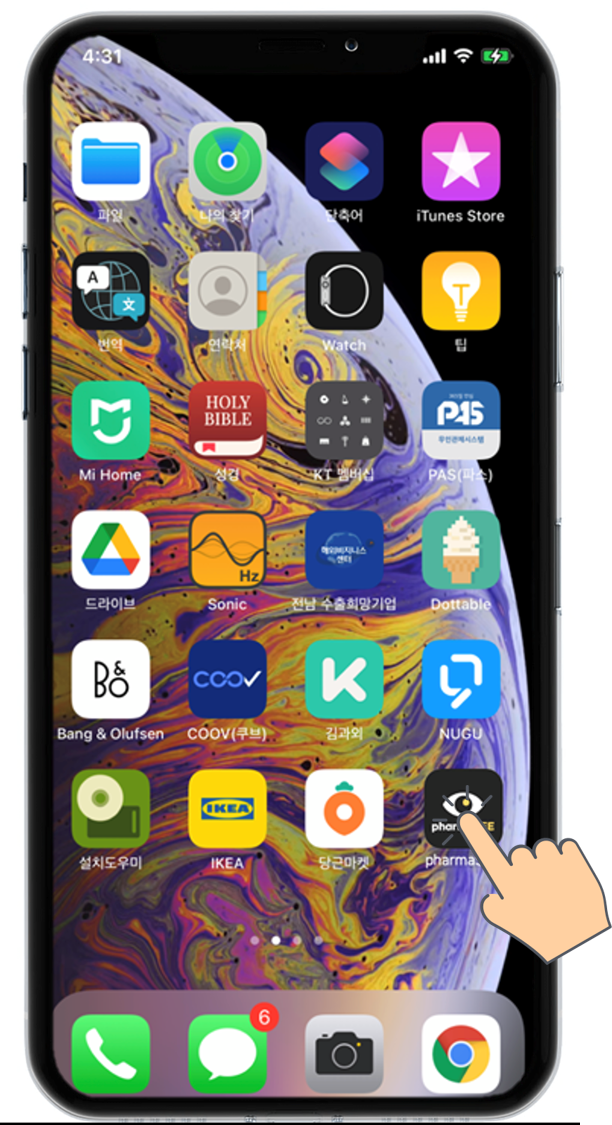
\includegraphics[width=5cm]{imagefolder/appstart.png}
\caption{}
\label{fig:map}
\end{figure}

\subsection{Loading}
When the user launches PharmaSEE, a loading page greets the user. The background of the loading page is a nature-friendly, self-made image composed of mountains, sun and stars with ice caps on an emerald background. There are two actions the user can take while the loading page is running.\\

\subsubsection{When a user waits}
If the user waits on the loading page, normal execution is possible and My Page appears first.\\

\subsubsection{When a user leaves}
If the user leaves the application without waiting on the loading page, the execution of PharmaSEE is terminated. After that, if you run the application again, you have to proceed with loading again.\\

\subsection{Main Page}

\subsubsection{User's Basic Information}
When loading is complete, the user first sees the main page. The main page shows the user's name and picture. Users can check the pills they need to take today and when to take them on the main page. Their availability is indicated by a green checkmark.\\

\paragraph{
If the square box has a green checkmark: }
If the square box has a green checkmark, the user has completed the dose correctly. \\

\paragraph{If the square box hasn't a green checkmark : }
If there is no green checkmark in the squared box, the user has not yet finished taking the dose and will need to take it in the future. \\

\subsubsection{Update Button}
When the user clicks the update button, his/her most recent pill taking information may be received from the server. \\

\subsubsection{Navigation Bar}
On the main page, the Navigation Bar appears at the top left with the user's basic information. When the user clicks the white navigation bar, the entire menu can be seen at a glance.There are two actions the user can take in relation to the Navigation Bar.\\

\paragraph{One click on the navigation bar}
If the user clicks the Navigation Bar once, the entire menu can be checked. If they click on another menu they will be able to go to that page.\\

\begin{figure}[h!]
\centering
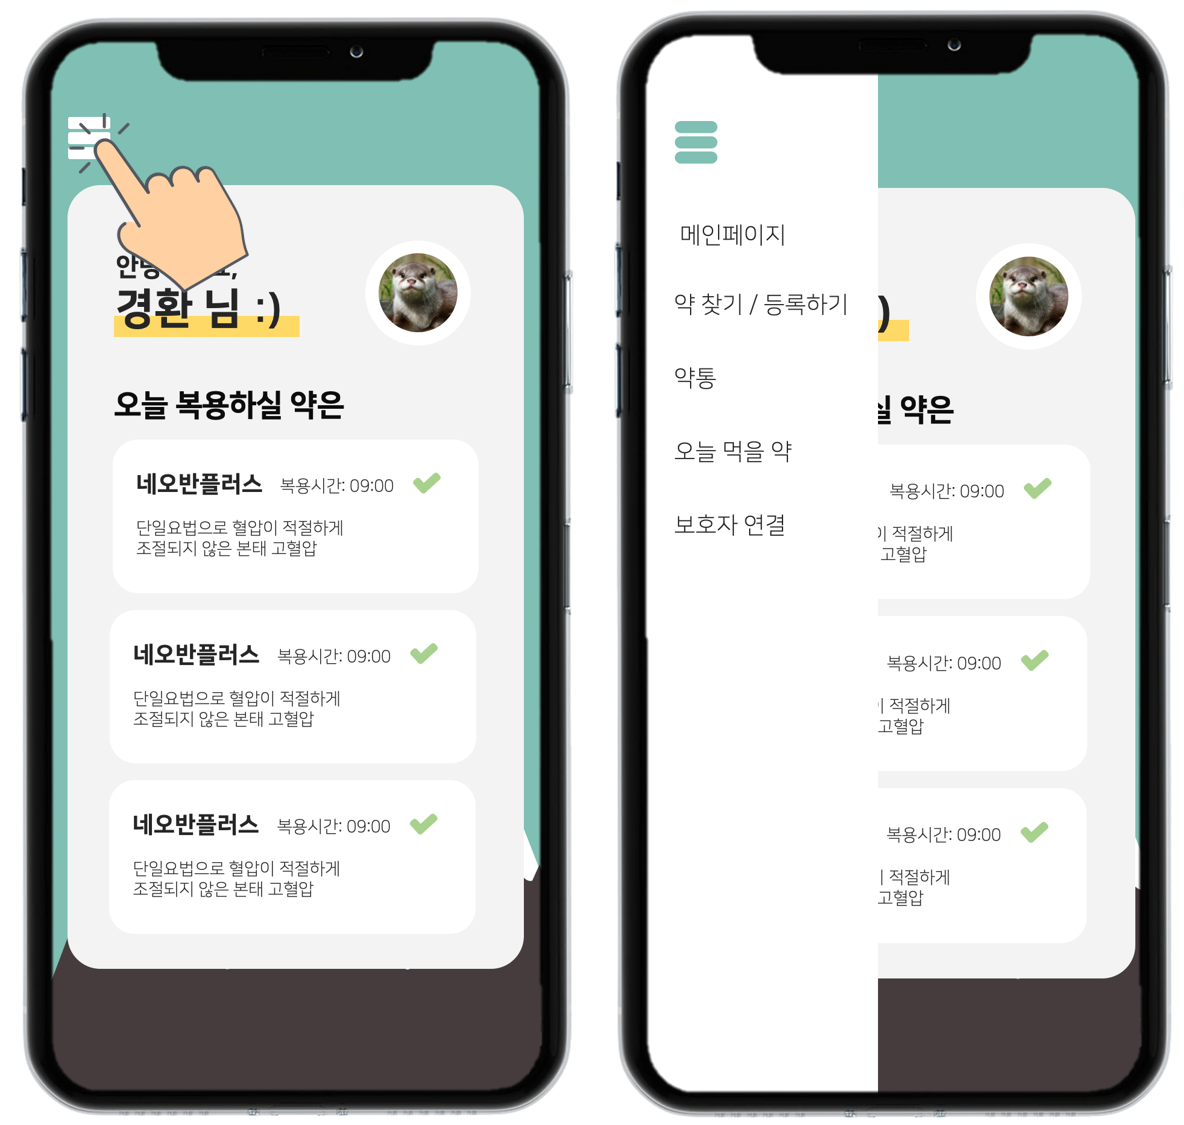
\includegraphics[width=5cm]{final_image_folder/click_navibar.png}
\caption{}
\label{fig:map}
\end{figure}

\paragraph{Double clicks on the navigation bar}
If the user double-clicks the Navigation Bar, the Navigation Bar that appears after clicking once disappears. \\

\begin{figure}[h!]
\centering
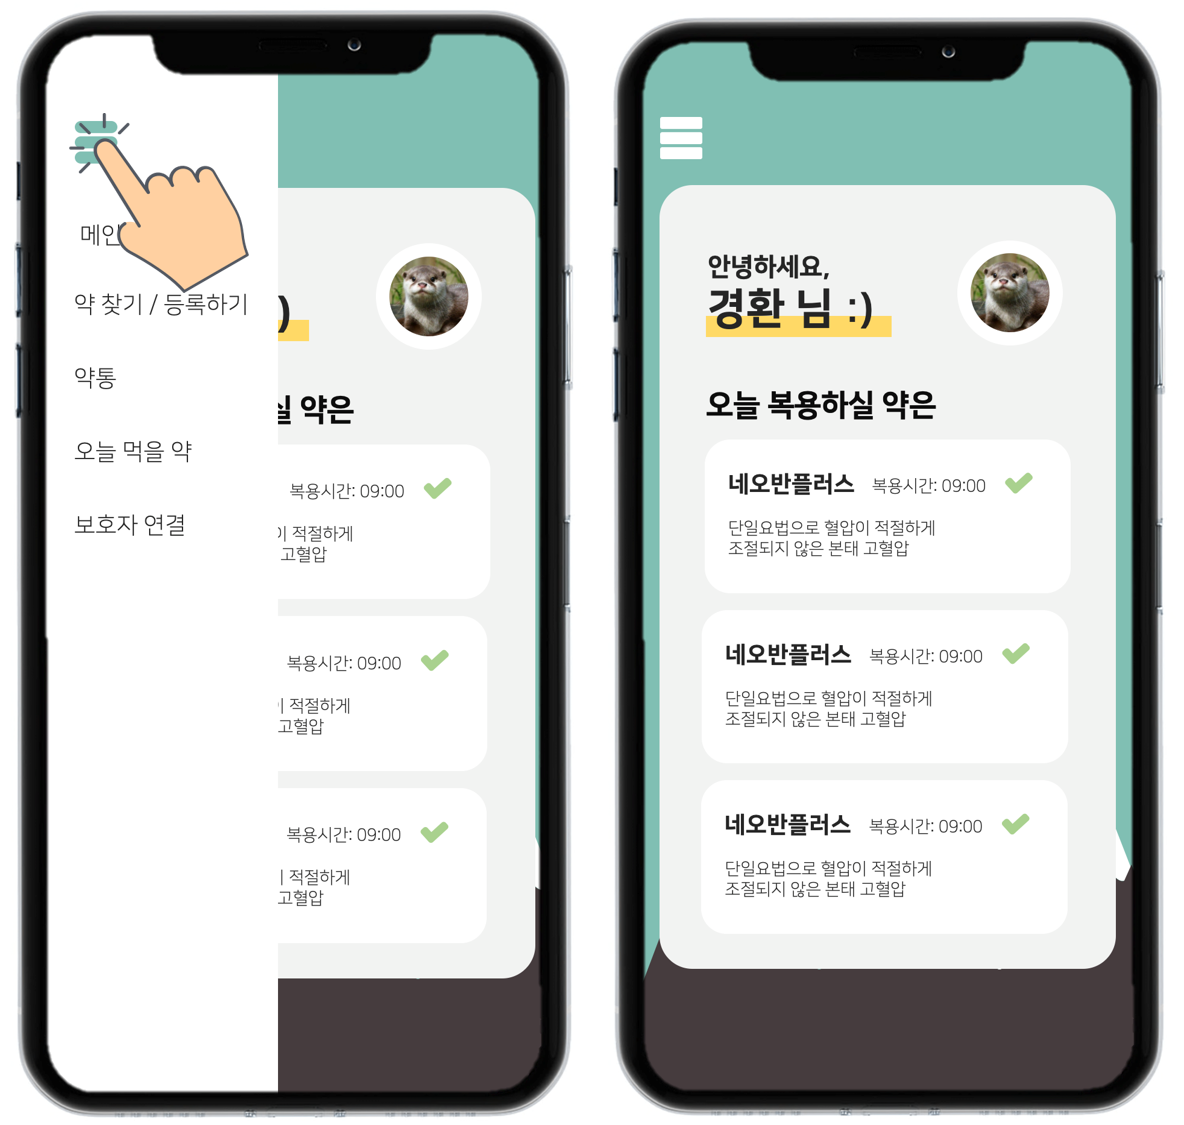
\includegraphics[width=5cm]{final_image_folder/click_mypage.png}
\caption{}
\label{fig:map}
\end{figure}

\subsection{Clicking Search/Register Pills}
If the user clicks 'Search/Register Pills' in the navigation bar, the user can go to the Search/Register Pills page. On this page, users can search for pills in three ways. The available methods are as follows.\\

\begin{itemize}
  \item Symptoms
  \item Names
  \item Photos\\
\end{itemize}

\begin{figure}[h!]
\centering
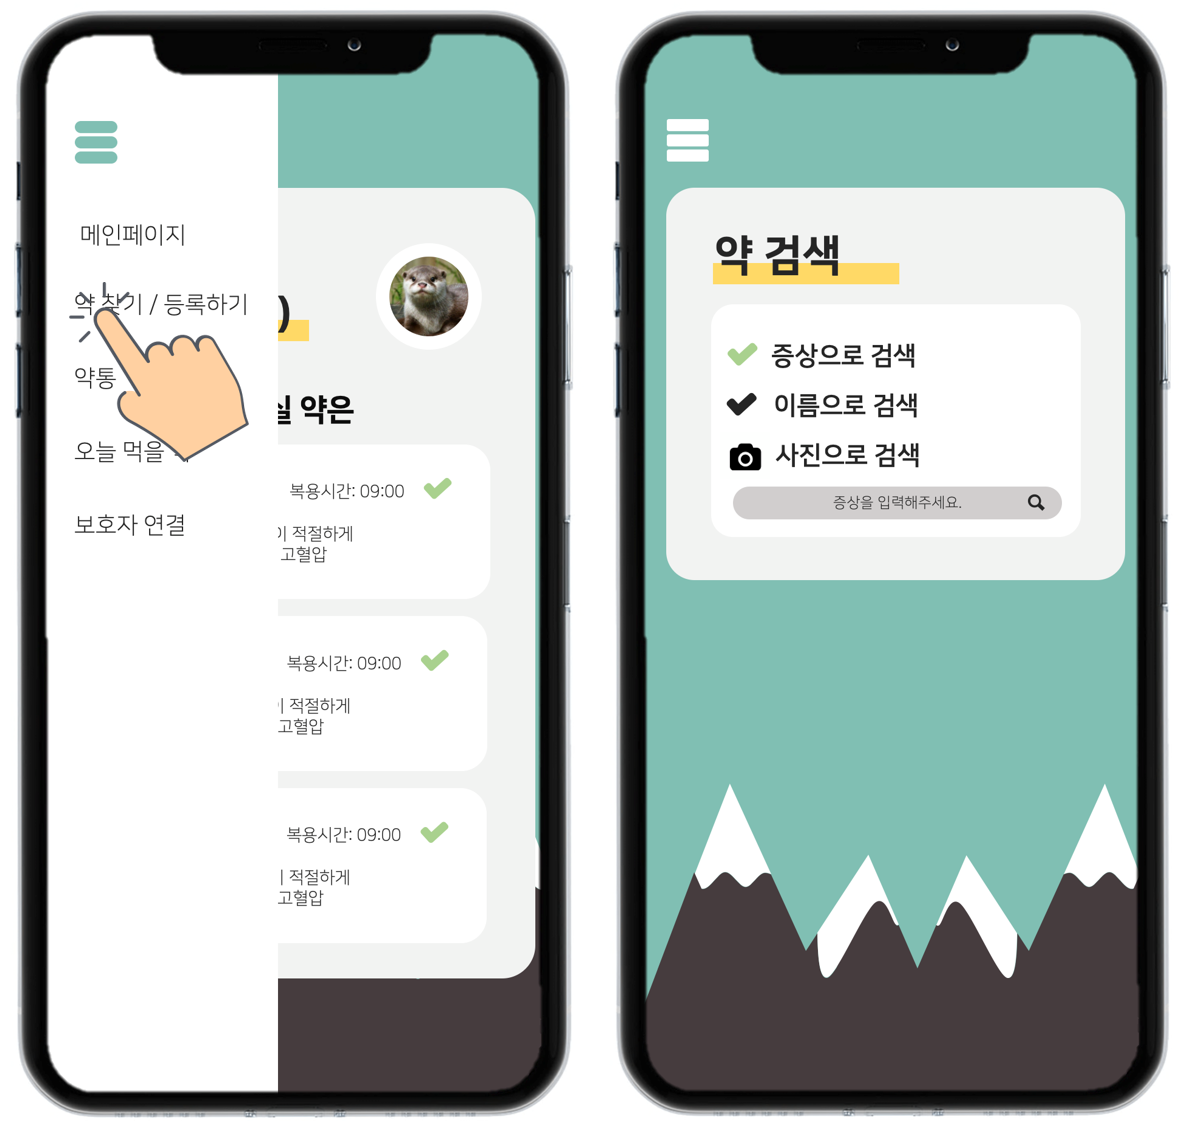
\includegraphics[width=5cm]{final_image_folder/click_search.png}
\caption{}
\label{fig:map}
\end{figure}

\paragraph{If the user has ever used the app}
When entering the page, the method the user has previously used is selected. \\

\paragraph{If a user uses the app for the first time}
'Search by symptoms' at the top is selected by default.\\

\subsubsection{Searching}

\paragraph{Selecting Search By Symptoms}

\subparagraph{
1. If the server has pill information related to the symptom: }
When the user inputs their symptoms, the pills related to them are listed. \\

\subparagraph{2. If the server does not have pill information related to the symptom: }
A text stating that there are no pills associated with the symptom the user entered appears.\\

\paragraph{Selecting Search By Names}

\begin{figure}[h!]
\centering
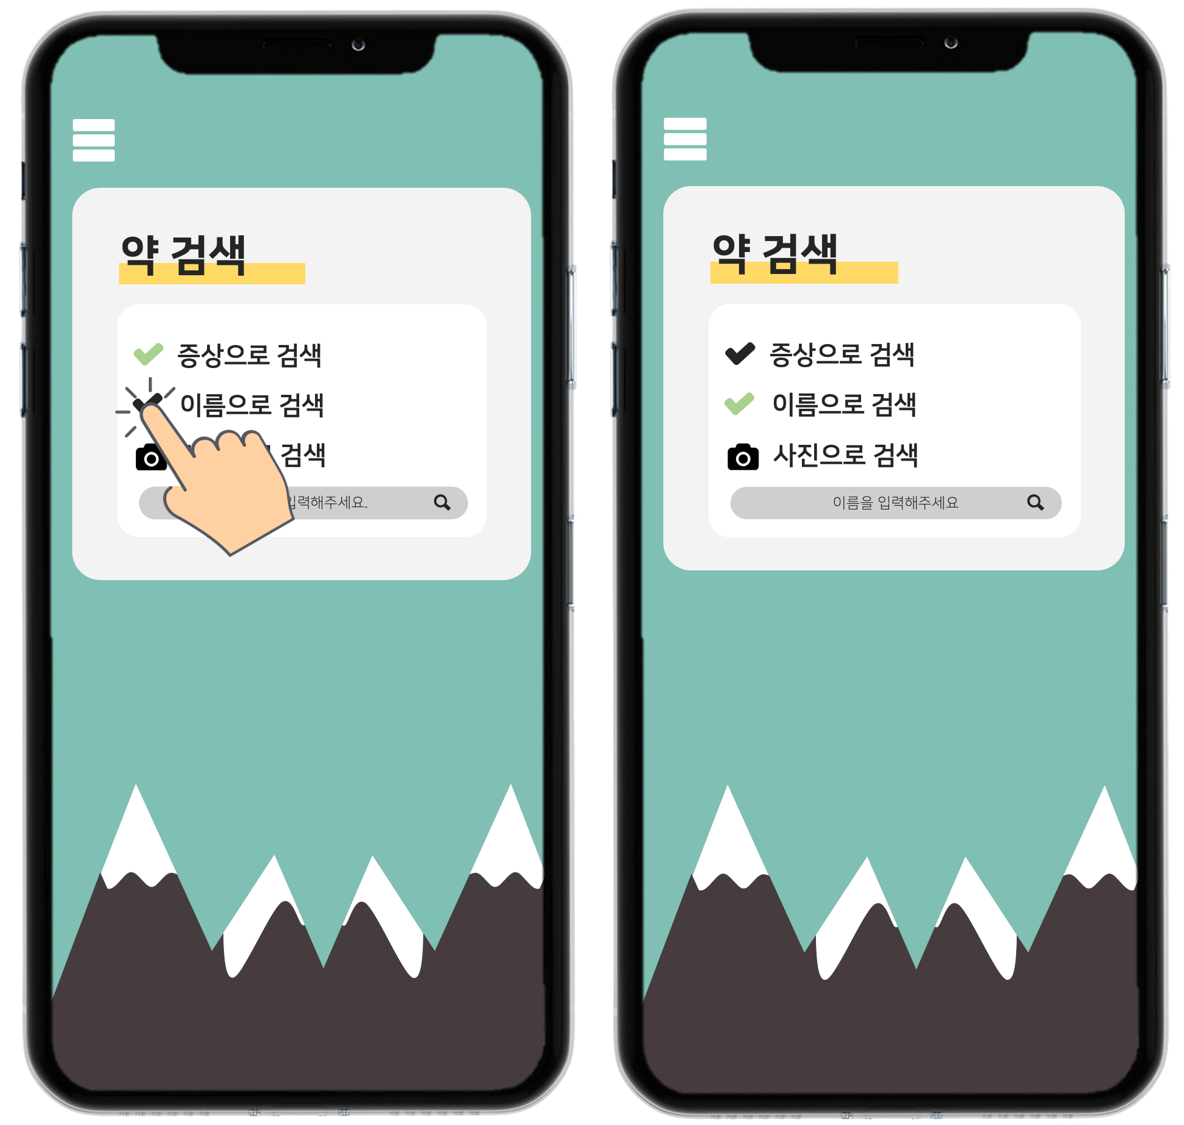
\includegraphics[width=5cm]{final_image_folder/click_search_name.png}
\caption{}
\label{fig:map}
\end{figure}

\subparagraph{
1. If the server has pill information related to the name: }
When the user inputs the name of the pill, the pills are listed in the order of the most similar names.\\

\subparagraph{2. If the server does not have pill information related to the name: }
A text stating that there are no pills associated with the name the user entered appears.\\

\paragraph{Selecting Search By Photos}
When the user presses search by photo, it can go directly to the camera. When a user takes a picture of a pill using a camera, the pills in the picture are analyzed.\\

\subparagraph{1. If the server has pill information related to the photo:}
Users can receive a list of medications in the photos they take.\\

\subparagraph{2. If the server does not have pill information related to the photo:}
A text stating that there are no pills associated with the picture the user took appears.\\


\\
\\
\begin{figure}[h!]
\centering
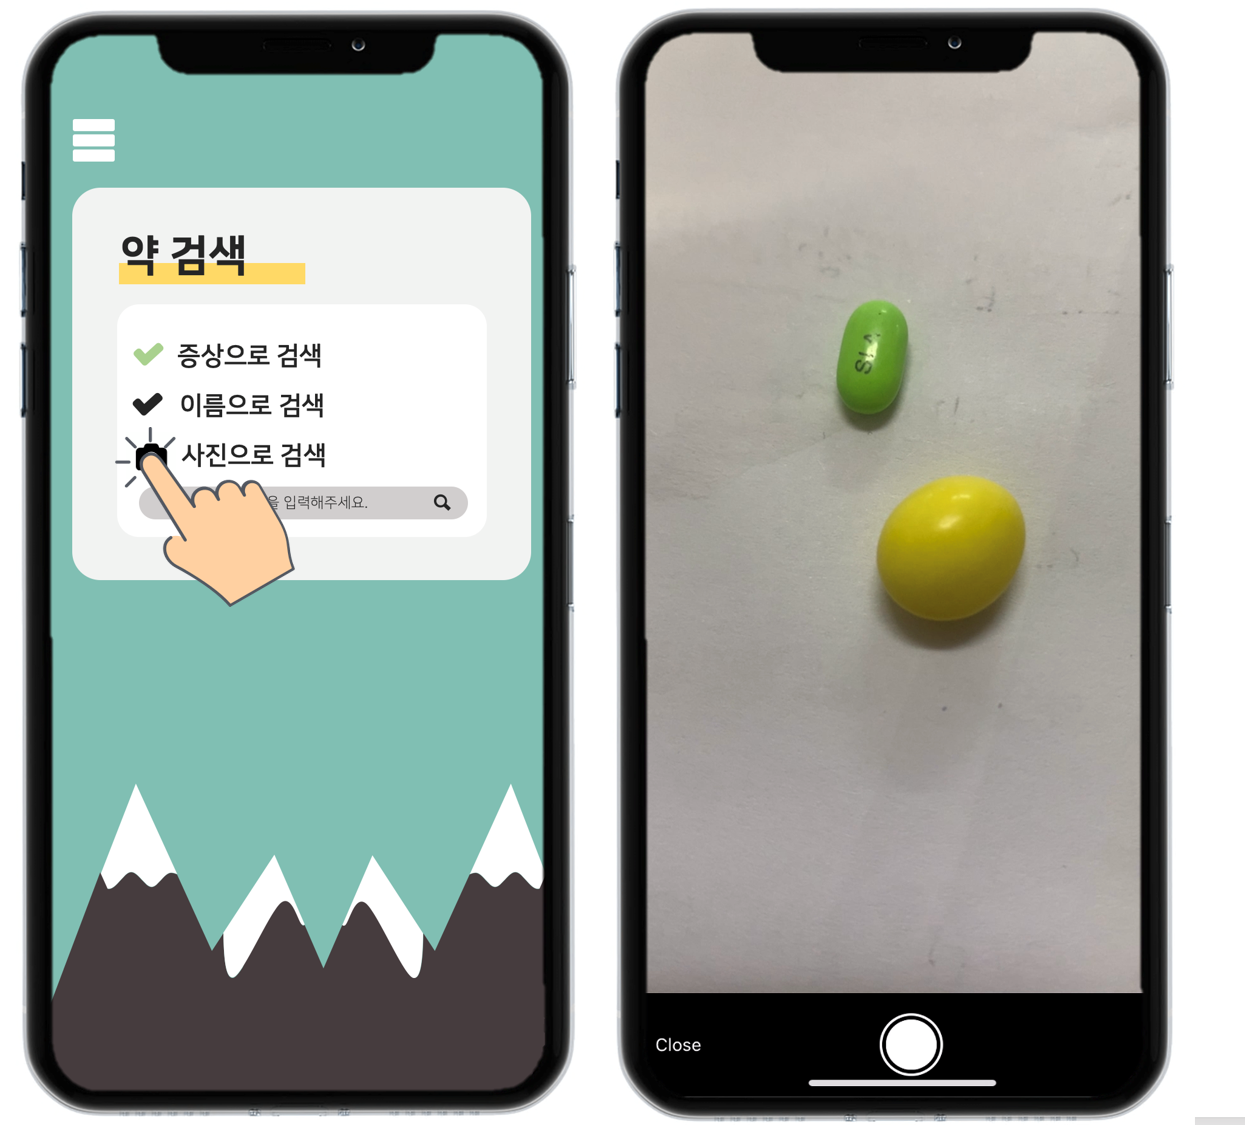
\includegraphics[width=5cm]{final_image_folder/click_search_photo.png}
\caption{}
\label{fig:map}
\end{figure}

\subsubsection{Adding To Pill Box}
When the user presses the 'Add to pill box' button, the corresponding pill can be added to their pill box. When they press the button, they get a notification saying 'Added to pillbox'. If users press the OK button they can return to the previous screen. If users don't click the OK button, they stay on the screen. \\

\begin{figure}[h!]
\centering
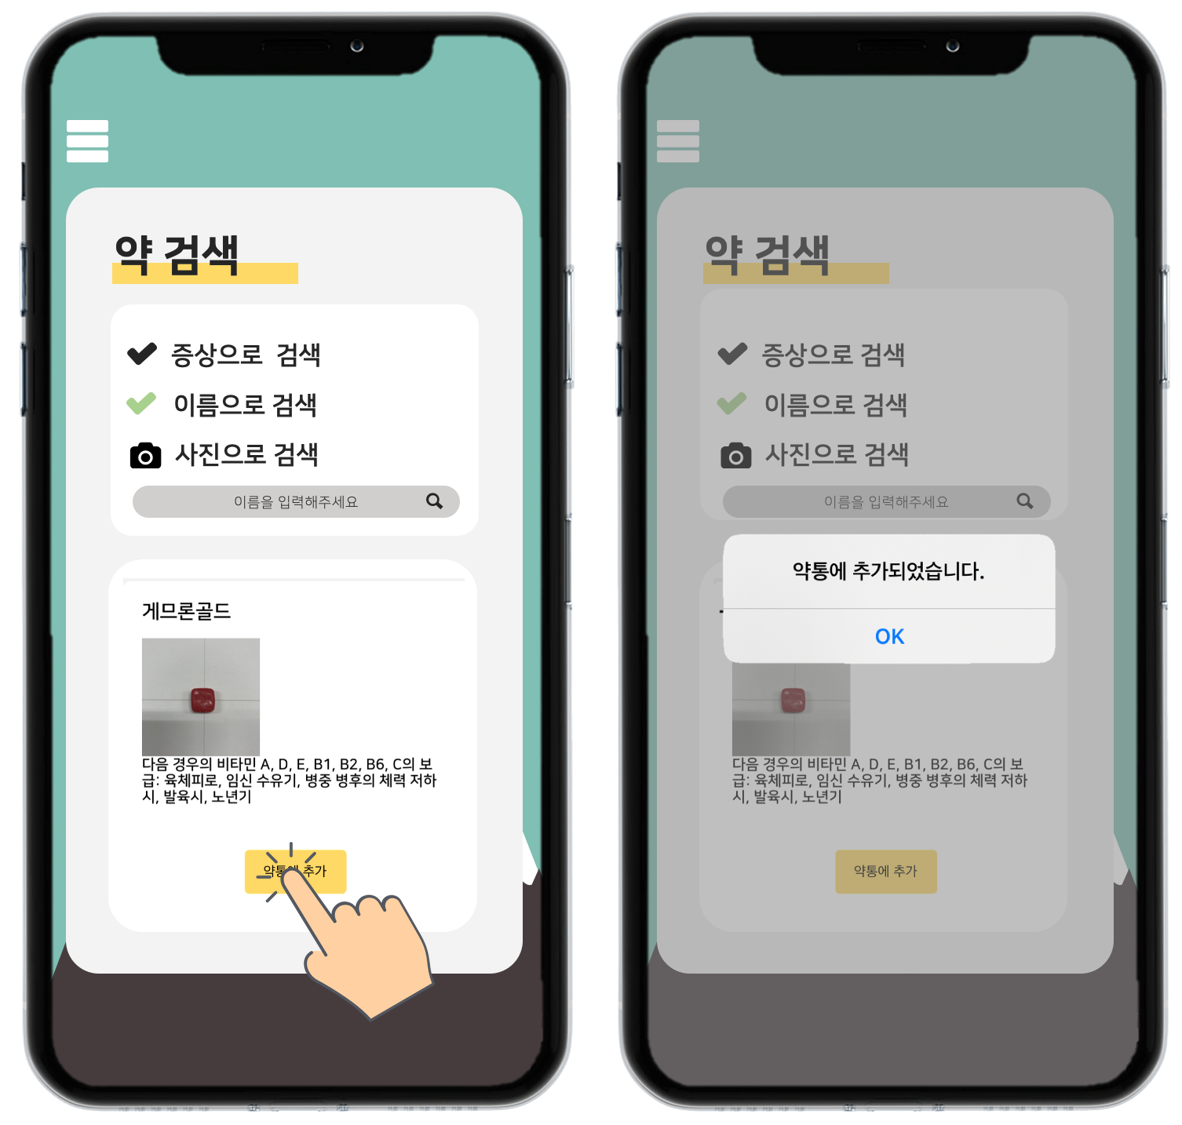
\includegraphics[width=5cm]{final_image_folder/click_search_add.png}
\caption{}
\label{fig:map}
\end{figure}

\subsection{Clicking Pill Box}
If the user clicks on the Pill Box on the navigation bar, it goes to that page. Users are divided into the following two cases.\\

\begin{figure}[h!]
\centering
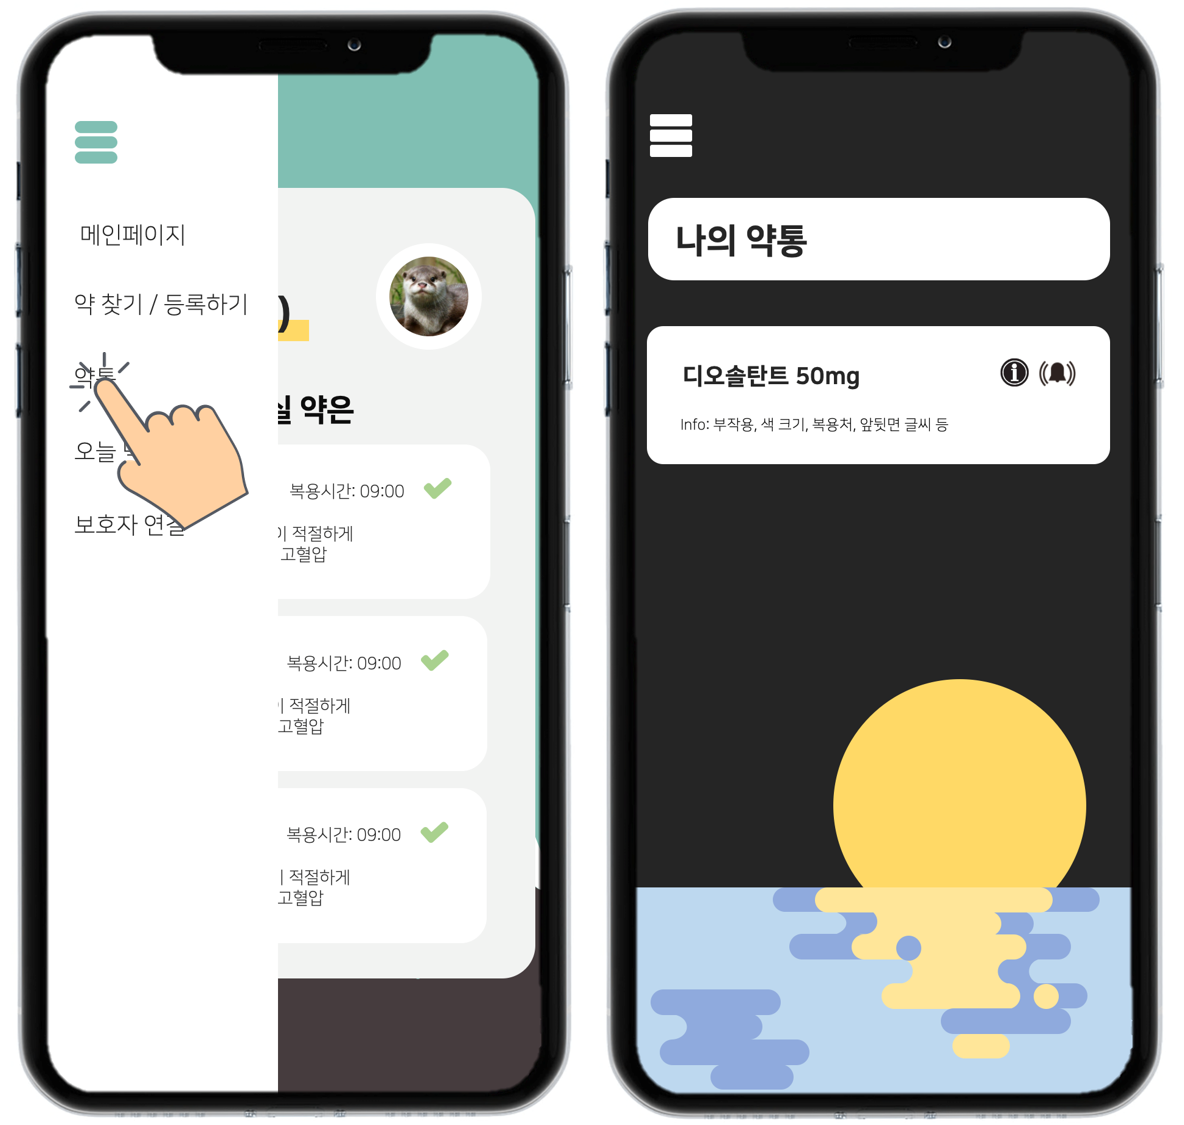
\includegraphics[width=5cm]{final_image_folder/click_pillbox.png}
\caption{}
\label{fig:map}
\end{figure}

\subsubsection{If the user has ever used the app}
If the user has ever used this app, two cases are possible.\\

\paragraph{If the user has ever added a pill to the medicine box}
If the user has added pills to the pill box, a list of pills the user has added appears. Each pill is represented in the form of a square box. The user sees the name, shape, color and function of each pill at a glance in a square box. Users can click three buttons inside each square box.\\

\subparagraph{1. Sign Board-shaped Icon:}
When the user clicks on the sign board-shaped icon, they can check a widen box which contains detailed information about each pill. If the users tab the icon again they can return to the previous screen.\\
\\
\\
\\
\begin{figure}[t!]
\centering
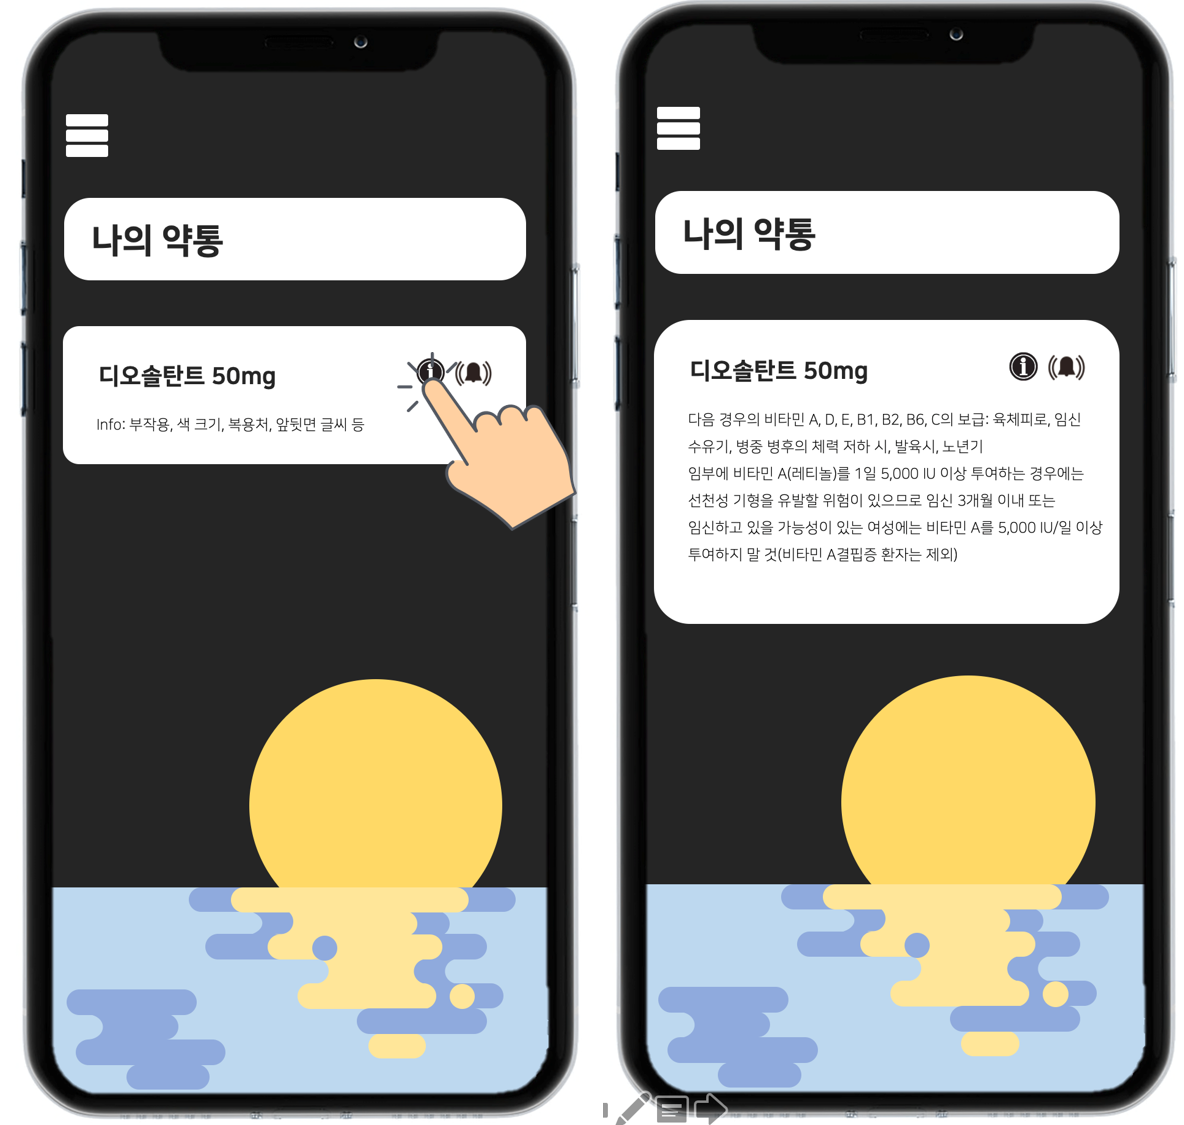
\includegraphics[width=5cm]{final_image_folder/click_pillbox_info.png}
\caption{}
\label{fig:map}
\end{figure}

\subparagraph{2. Bell-shaped Icon:}
When the user clicks on the bell shaped icon, it goes to a page where you can set an alarm for each pill taking. The user can set the following two settings. After they set the alarm, press the bell again to save the alarm and return to the previous screen. \\

\begin{itemize}
  \item Taking Time
  \item Taking Duration\\
\end{itemize}

\begin{figure}[h!]
\centering
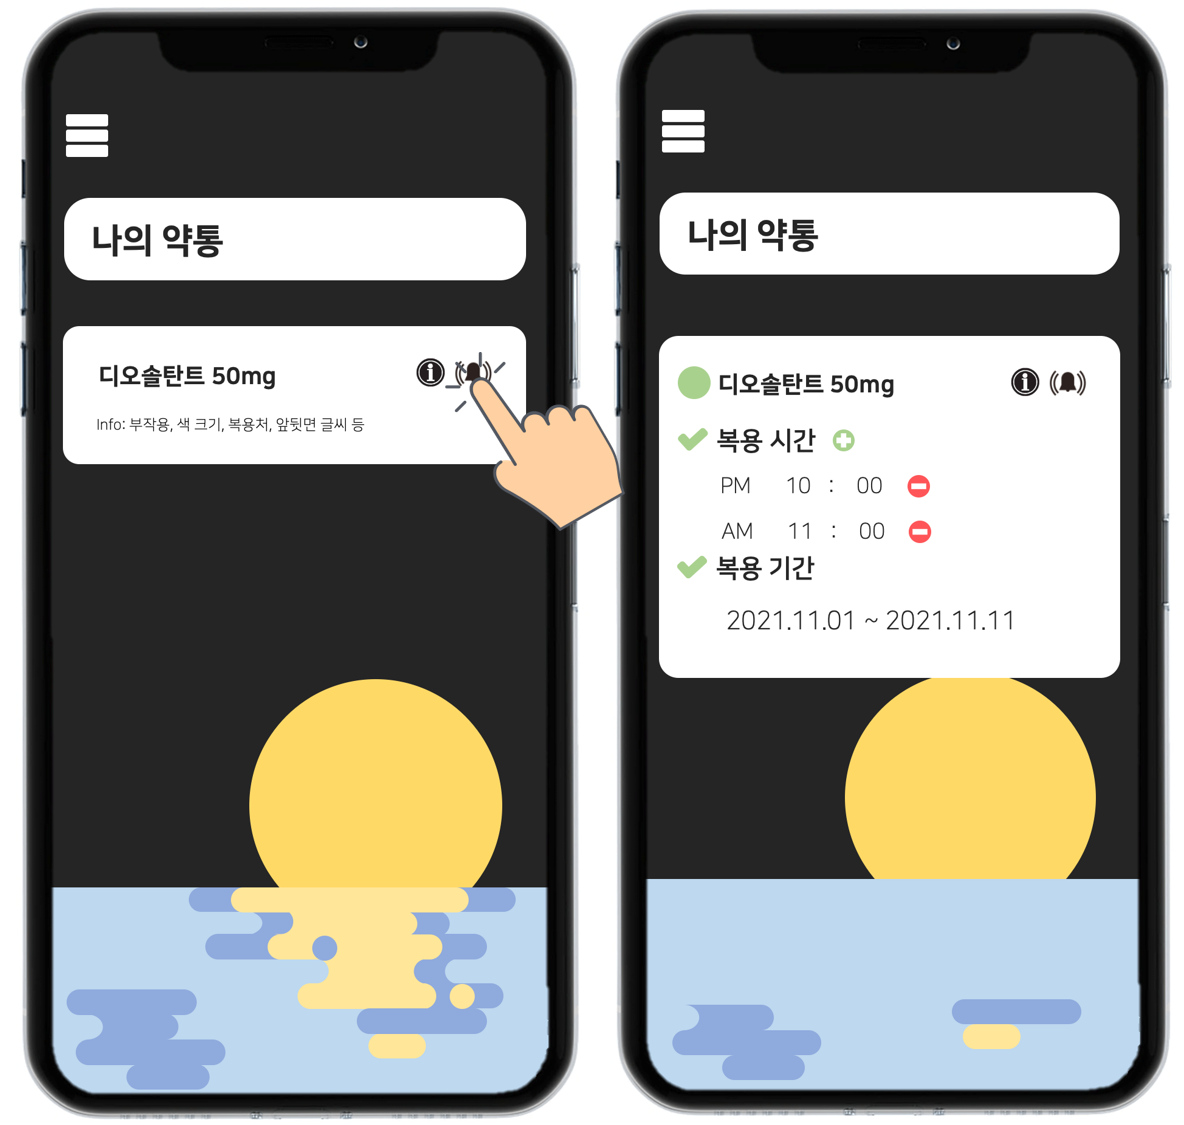
\includegraphics[width=5cm]{final_image_folder/click_pillbox_alarm.png}
\caption{}
\label{fig:map}
\end{figure}

\subparagraph{a. Taking Time: }
In the Taking Time, users can click two buttons. \\

\subparagraph{aa. Clicking + Button: }
By clicking on the + button, the user can add a dosing time. If they click the green + button, a pop-up will appear allowing you to add a new alarm. Alarms can be added when users enter a time in a specified format and press OK. If they click Cancel, they go back to the previous page without adding a new alarm.  \\
\\
\\
\\
\\
\\
\\

\begin{figure}[t!]
\centering
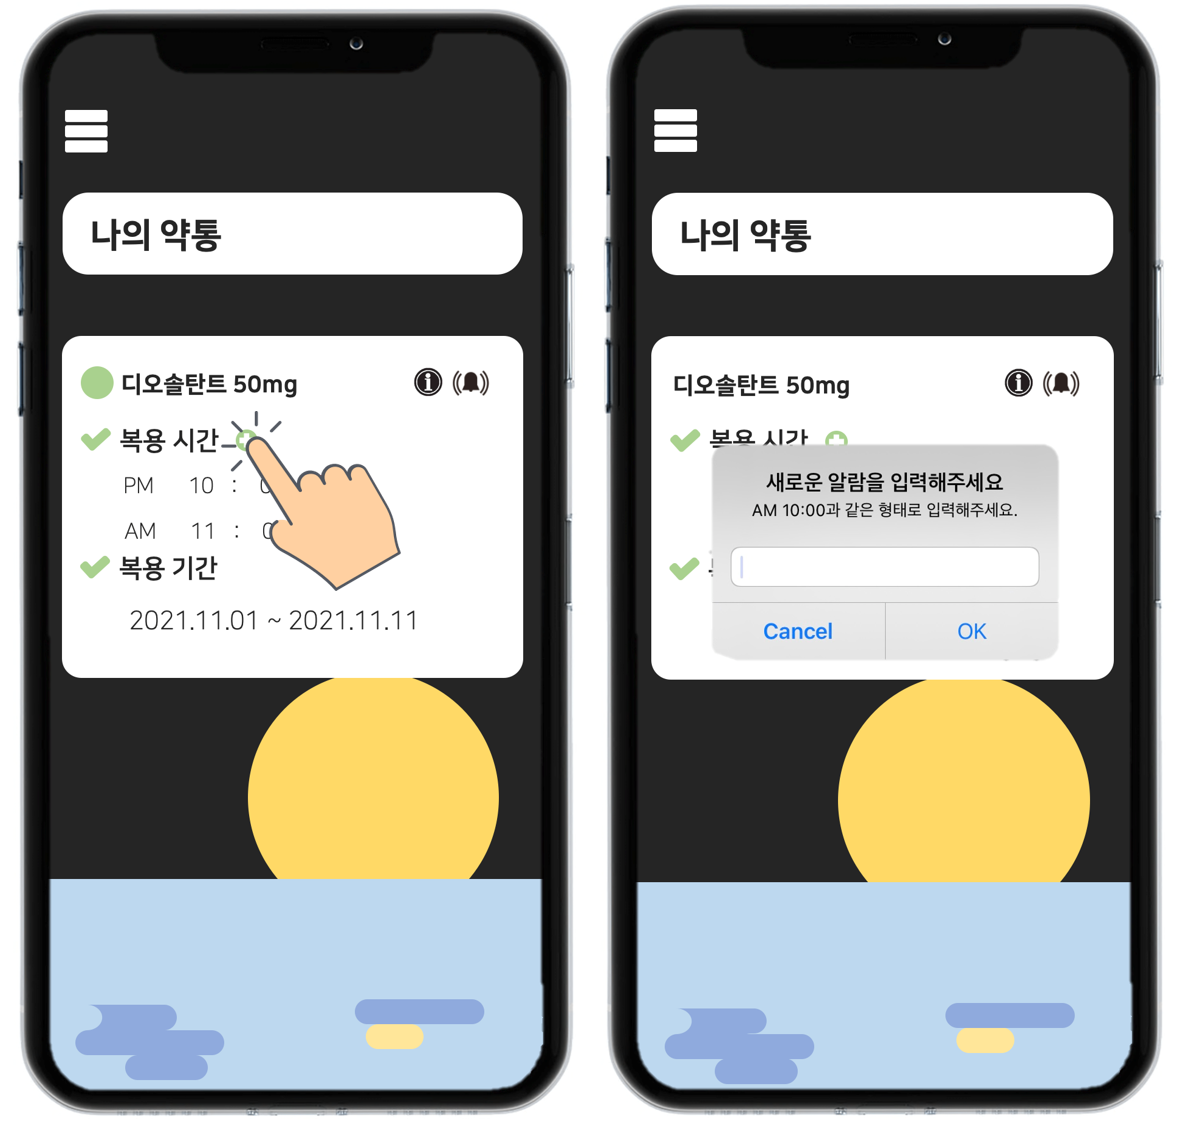
\includegraphics[width=5cm]{final_image_folder/click_pillbox_alarm_add.png}
\caption{}
\label{fig:map}
\end{figure}

\subparagraph{ab. Clicking - Button: }
If the users click the - shape button, they can delete the dosage alarm entered by them. When users press the red minus button, a pop-up appears asking if they really want to delete the alarm. When they click yes the alarm is really cleared. If they click No, the alarm will not be deleted, and you will be returned to the previous page without any changes.\\

\begin{figure}[h!]
\centering
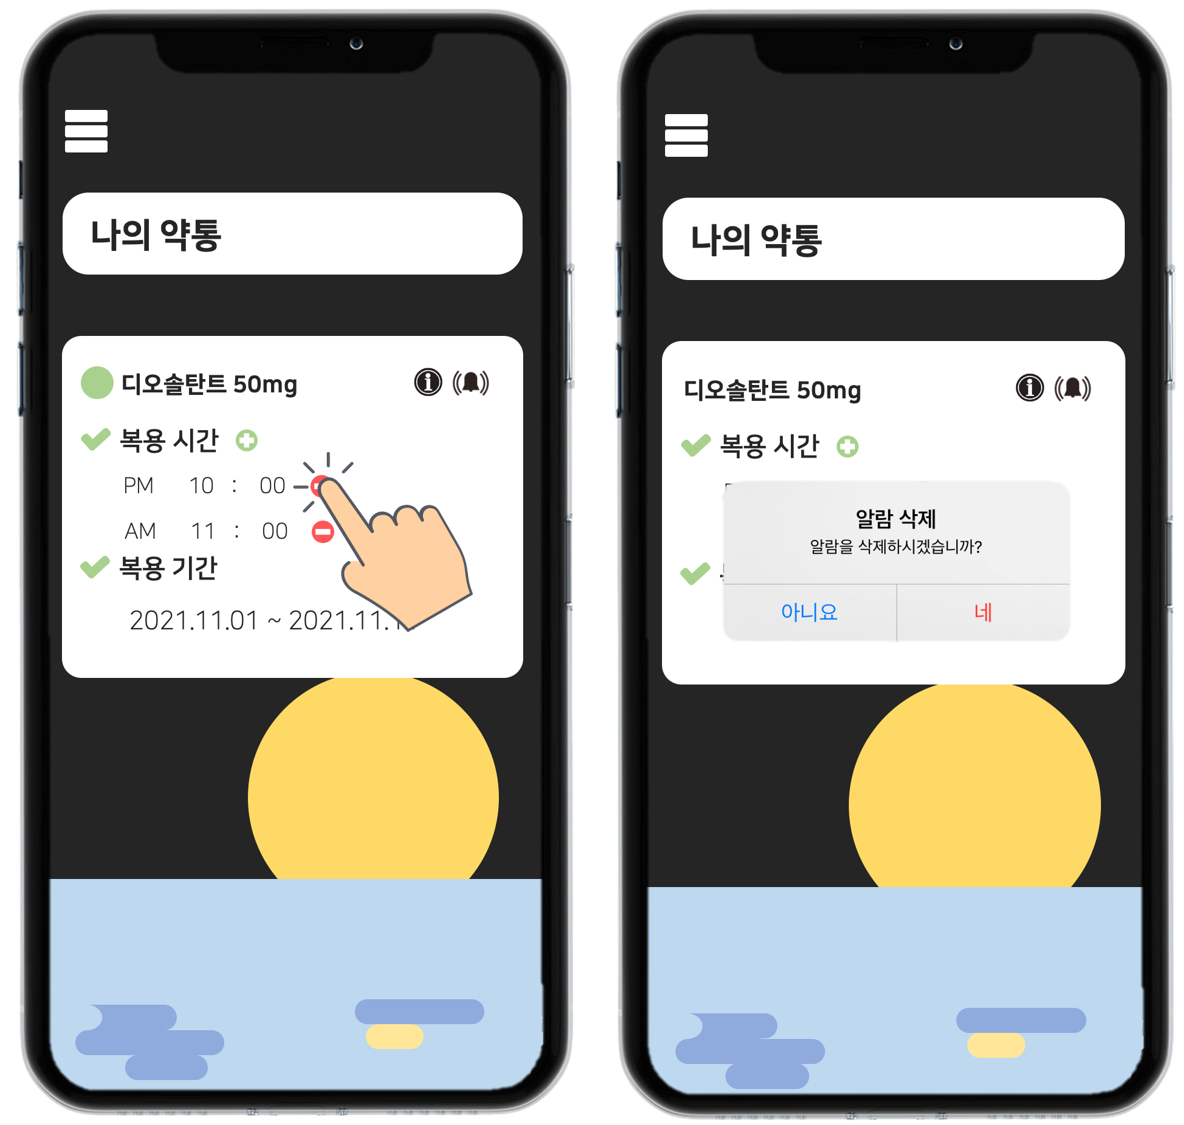
\includegraphics[width=5cm]{final_image_folder/click_pillbox_alarm_remove.png}
\caption{}
\label{fig:map}
\end{figure}

\subparagraph{b. Taking Duration: }
In the Taking Duration, users can enter the length of time they take the medicine. The date before the ~ is the start date of taking. The date after the ~ is the end date of the dose. If the period ends, the pill disappears from the list.\\

\paragraph{If the user has never added a pill to the medicine box}
If the user has not added pills to the pill box, no list will appear.\\

\subsubsection{If a user uses the app for the first time}
If a user uses the app for the first time, no list will appear.\\

\subsection{Clicking Today's Pill}
When a user clicks Today's Pill in the navigation bar, they are taken to that page. The situation can be divided into two processes. Users can check whether the pills they are preparing to eat are the correct ones to take now by sending photos to the server. \\

\begin{figure}[h!]
\centering
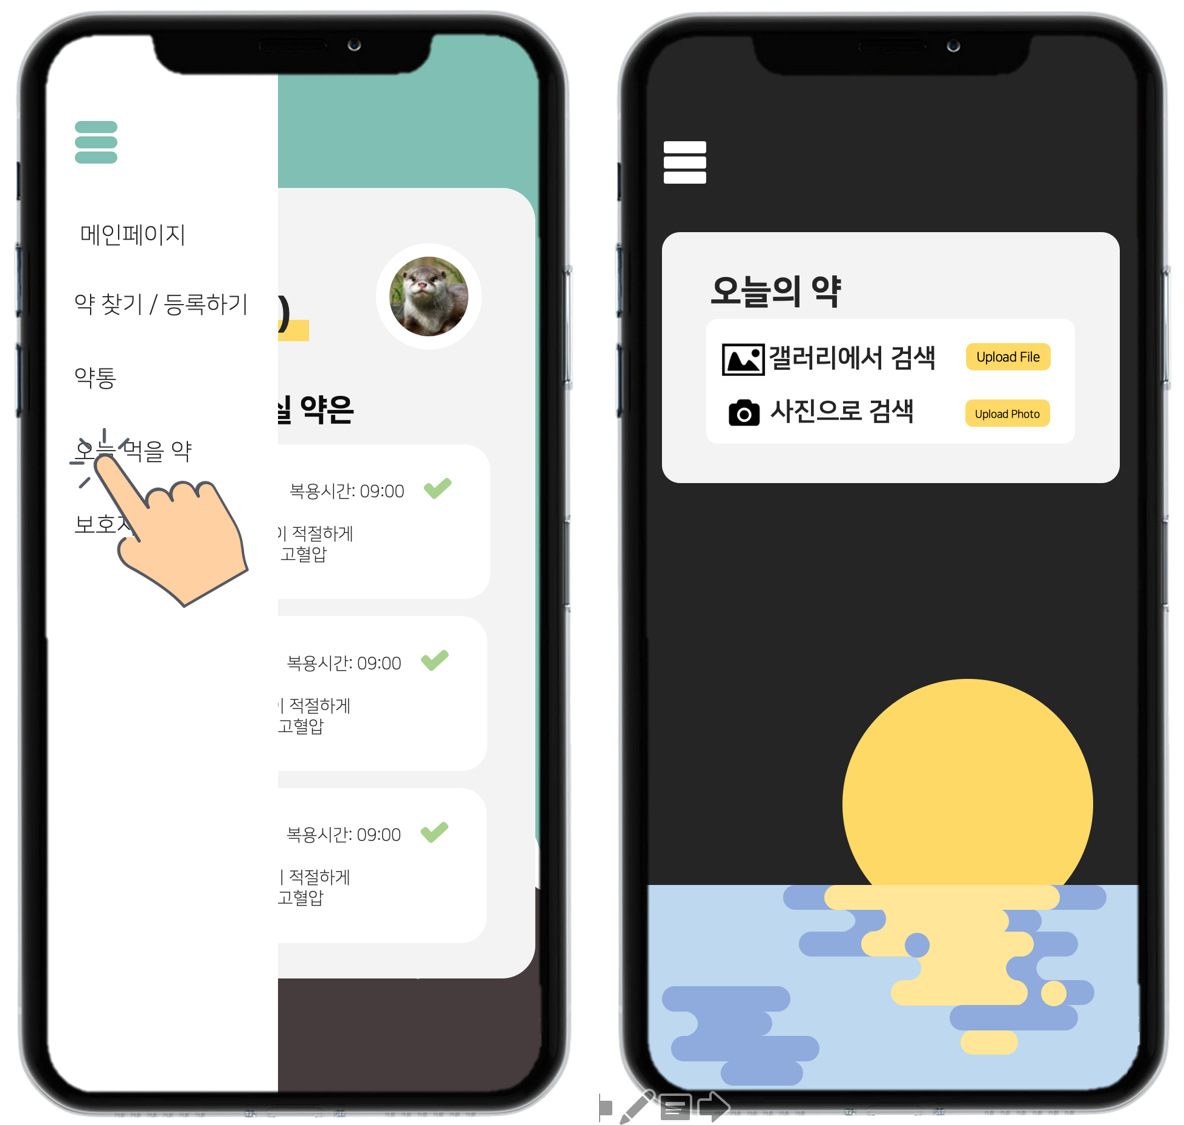
\includegraphics[width=5cm]{final_image_folder/click_today.png}
\caption{}
\label{fig:map}
\end{figure}

\subsubsection{When The Users Sends Photos To The Server}
Users can send photos to the server in two ways. The first is 'Search In Gallery' and the second is 'Search By Photo'. \\

\paragraph{When The Users Choose Search In Gallery}
When the user clicks 'Search In Gallery', it moves directly to their own gallery. Users can select the picture of the pills they are about to take. After entering a photo, if they click 'Upload File', the photo is sent to the server.

\paragraph{When The Users Choose Search By Photo}
When the user clicks 'Search By Photo', it moves directly to the camera. Users can use the camera to take pictures of the pills they are about to take. After taking a photo, if they click 'Upload Photo', the photo is sent to the server.\\

\subsubsection{When The Users Receive Pill Analysis Results}
If users have a little waiting time, they can get a picture back from the server containing the analysis result of the pill in the picture. Before users can see the photo, a pop-up will be shown telling them to take the correct pill. Hit 'OK' in the pop-up, and they will immediately see a picture of the result. If it is a medicine to be taken today, a green checkmark will appear on the medicine, and if it is not a medicine to be taken today, a red X will appear on the medicine. Users can distinguish which medicines they need to take through the returned photos and the different colored marks. If they want to try again, they can click Take Photo or Upload Photo again without resetting.\\

\begin{figure}[h!]
\centering
\includegraphics[width=5cm]{final_image_folder/click_today_photo.png}
\caption{}
\label{fig:map}
\end{figure}

\begin{figure}[h!]
\centering
\includegraphics[width=5cm]{final_image_folder/click_today_ok.png}
\caption{}
\label{fig:map}
\end{figure}
.\\
\\
\\
\\
\\
\\
\\
\\
\\

\subsection{Clicking Link Caregivers}
When a user clicks Link Caregivers in the navigation bar, they are taken to that page. If users come to the Link Caregivers page, they can see the caregiver search bar. Users can search by entering the caregivers' name in the name search box. Two different situations can occur.\\

\begin{figure}[h!]
\centering
\includegraphics[width=5cm]{final_image_folder/click_bohoja.png}
\caption{}
\label{fig:map}
\end{figure}

\subsubsection{If The User Entered In The Search Box Exists}
If there are users who typed in the search bar, they can follow them. After that, caregivers who have been followed can check the pill intake history of the wards who is their following. If the wards click the yellow 'Follow' button, they can get a notification that says 'Your follow request has been processed.'. They can go back to the previous page by clicking 'OK' button. If they don't click the button, they will stay at the page.\\

\begin{figure}[h!]
\centering
\includegraphics[width=5cm]{final_image_folder/click_bohoja_follow.png}
\caption{}
\label{fig:map}
\end{figure}

\subsubsection{If The User Entered In The Search Box Does Not Exist}
If the user entered into the search box does not exist, users will be notified that there is no user with that name.\\

\subsection{Clicking Return To Main Page} 
If users press return to main page in the navigation bar, they can return to main page.\\

\subsection{Turning Off The Application}
If users want to turn off the application, swipe down on the smartphone screen and then swipe up to close the application. Then, if they run PharmaSEE again, they start from scratch.\\

\subsection{Asking Nugu 'What pills did I take today?'}
If users ask the Nugu device questions such as 'What pills did I take today?', the Nugu device will respond with the information delivered from the backend proxy server.\\

\subsubsection{When there are no registered reminders}
If the user has no reminders registered, the Nugu will respond \\ 
'You (He/She if the user is the caretaker) have no reminders registered.' or 'You (He/She if the user is the caretaker) have no pills scheduled yet. Please check from the PharmaSEE mobile application.'\\

\subsubsection{When there are pills taken today}
If the user has reminders registered, and took the pills today, Nugu will respond \\ 
'You (He/She if the user is the caretaker) took {number of dose} doses of {pill name} at 8am today.' \\ \\
If there are several pills taken at the same time, Nugu's response will be something like \\ 
'You (He/She if the user is the caretaker) took 2 doses of pillA, 1 dose of pillB a 8am today.'. \\ \\
As you can see, if the time taken is identical, the pill intake information will be grouped by taken time and spoken together.\\

\subsubsection{When there are pills that were taken more than 2 hours later/faster than scheduled time}
If the user took the pills registered in the reminders, but the time they took it differs from the scheduled time by more than 2 hours, Nugu will inform them by adding a caution message to the prompt. For example, if the user took pillA at 10:30pm, when the scheduled time was 8pm, Nugu will add to the respond \\ \\
'You (He/She if the user is the caretaker) took 2 doses of pillA 2 hours later/earlier than the scheduled time.'

\subsection{Asking Nugu 'What pills did I not take today?'}
If users ask the Nugu device questions such as 'What pills did I not take toady?' or 'Are they any pills I forgot today?', the Nugu device will respond with the information delivered from the backend proxy server. \\

\subsubsection{When there are no registered reminders}
If the user has no reminders registered, Nugu will respond  \\ \\
'You (He/She if the user is the caretaker) have no reminders registered.' or 'You (He/She if the user is the caretaker) have no pills scheduled yet. Please check from the PharmaSEE mobile application.'\\

\subsubsection{When there are pills overdue intake time}
If there are pills that were scheduled to be taken but not taken yet, they will be listed as overdue pills. Nugu will try to remind the user that their is an overdue medication by prompting a respond looking like \\ \\ 
'You (He/She if the user is the caretaker) forgot to take 2 doses of pillA, 1 dose of pillB at 8am. Please open the PharmaSEE mobile app to confirm.'\\

\subsubsection{When there are pills scheduled later that day}
If there are pills that are scheduled in the future and not taken yet, they will be listed as scheduled pills. Nugu will inform the user that there is an medication that has to be taken at a coming time today. The response will be like \\ \\ 
'You (He/She if the user is the caretaker) are scheduled to intake 2 doeses of pillA at 7pm today. Please do not forget!'\\

\section{Installation Guide}
When a user searches for keywords such as pills, pill taking, pill management, health or parental health in the Apple App Store or Google Play Store, our application appears in the list. When they click on PharmaSEE's install button in the store, our application is downloaded to the user's smartphone. \\

\section{Conclusion}
PharmaSEE can help people who often forget when and how to take their pills correctly. In addition, it helps the caregivers effectively and efficiently manage whether or not their wards, such as the elderly or patients, who have more difficulty taking pills are taking the pills. In particular, it can further expand its customers by providing voice service support through an artificial intelligence speaker for people who have difficulty seeing the phone screen properly.\\ 

Also, PharmaSEE has the following expansion possibilities \\

\begin{itemize}
  \item It can recommend medications according to user's symptoms.\\
  \item It may be possible to prevent diseases beyond administration.\\
  \item If non-face-to-face prescription services are permitted, a caregiver can help the ward order medicine through it.\\
  \item Depending on the expansion of the data set, the range of supported drugs can be expanded and the performance of the pill detection model can be improved.\\
  \item It can identify and inform users about the side effects of taking drugs together, or tell the users which drug will work better when they add a new drug.\\
  \item It is scalable to a solution that connects with a doctor and manages the patient's continuous and safe medication.\\
  \item It can recommend or recognize a candidate group when an image is recognized without a drug in its entirety.\\
\end{itemize}

PharmaSEE aims to become a comprehensive drug management system with a wider scope using artificial intelligence and voice recognition technology in the future. \\

\end{document}
